%==============================================================================
%  FACE-ATLAS — A latent atlas of severe mental illness
%  One comprehensive, discovery-framed manuscript (Gaussian-copula vertical).
%
%  Build:  pdflatex main -> bibtex main -> pdflatex main -> pdflatex main
%
%  Journal-agnostic (Nature-family / Lancet Psychiatry convertible). Results-first
%  discovery framing; high-level model in the main text, full derivation in the
%  Annexes (\appendix). Author list / ethics / funding are PI placeholders.
%==============================================================================
\documentclass[11pt]{article}

\usepackage[utf8]{inputenc}
\usepackage[T1]{fontenc}
\usepackage{lmodern}
\usepackage[a4paper,margin=1in]{geometry}
\usepackage{amsmath,amssymb,amsthm}
\usepackage{graphicx}
\usepackage{booktabs}
\usepackage{array}
\usepackage{multirow}
\usepackage{rotating}
\usepackage{xcolor}
\usepackage{microtype}
\usepackage[hidelinks]{hyperref}
\usepackage[numbers,sort&compress]{natbib}

\graphicspath{{figures/}{../docs/figures/}}

\newcommand{\Gfac}{\textit{G}}            % the general functional-burden factor
\newcommand{\orth}{\ensuremath{\perp}}    % orthogonality, usable in text
\newcommand{\todo}[1]{\textcolor{red}{[\textbf{TODO:} #1]}}

% Annex theorem-like environments (proofs live in the Annexes only)
\newtheorem{proposition}{Proposition}
\newtheorem{lemma}{Lemma}
\newtheorem{corollary}{Corollary}

% Extended Data figure numbering helper
\newcommand{\edfig}[1]{Extended Data Fig.~\ref{#1}}

\title{\bfseries A latent atlas of severe mental illness separates biological
burden from clinical severity and forecasts functional outcome}

\author{%
  Andrii Kulakovskyi$^{1,2}$\ \and \emph{[co-authors / FACE--FondaMental investigators TBD]}%
  \thanks{Correspondence: andrii.kulakovskyi@gmail.com}%
}
\date{%
  $^{1}$Precision Psychiatry \& Artificial Intelligence \quad
  $^{2}$[Institution TBD]\\[4pt]
  \today
}

\begin{document}
\maketitle

%================================ ABSTRACT ====================================
\begin{abstract}
\noindent
Psychiatric diagnoses aggregate biologically heterogeneous patients, which limits
mechanistic stratification and prognosis. We analysed the harmonized baseline
assessment of $N=9{,}013$ patients with bipolar disorder, schizophrenia or major
depression from the three FACE expert-centre cohorts using one global,
missingness-aware Bayesian bifactor / exploratory structural-equation model,
\emph{derived and fit to each patient's observed cells only} (no imputation), with
diagnosis withheld from model fitting. The model resolved a transdiagnostic
coordinate system: a general functional-burden factor (\Gfac) and eight specific
dimensions---cognition, metabolic load, inflammation, sleep, developmental risk,
suicidality, mania and substance use. The central finding is a \textbf{dissociation
between biology, symptoms and functional burden}: metabolic and inflammatory load
were the \emph{least} burden-entangled domains (correlation with \Gfac{} of $0.12$
and $0.07$, versus $0.39$ for cognition and $0.42$ for sleep), and they remained so
after adjustment for medication, adiposity and site. The coordinate space was a
graded \textbf{continuum, not discrete biotypes}---apparent clustering was
reproduced by a single-Gaussian null (best silhouette $0.140$ vs $0.141\pm0.002$,
$z=-0.36$)---yet four archetypal extremes gave a clinically legible reading,
including a \emph{biological} corner and a \emph{severe, non-biological} corner with
comparable functional burden but opposite biological profiles. Scored forward onto
follow-up without re-estimation, biological coordinates were stable (test--retest
intraclass correlation $0.91$ for metabolic load) whereas symptom axes were
state-like. The archetype phenotype predicted two-year functioning beyond diagnosis,
baseline severity and baseline functioning (held-out expected log predictive density
$+59$; two-year functional-remission $27\%$--$60\%$ across corners), but the
individual-level discrimination gain was small (remission AUC $+0.011$) and treatment
moderation was not demonstrated on observational, expert-centre treatment-as-usual
(lithium in bipolar disorder a well-identified null). These results define a
transdiagnostic biological atlas of severe mental illness that supports mechanistic
stratification and group-level functional forecasting, and they delineate the
requirements for clinical utility: external validation, incident-event outcomes and
randomized treatment data.
\end{abstract}

\noindent\textbf{Keywords:} transdiagnostic psychiatry; dimensional
psychopathology; bifactor model; metabolic syndrome; inflammation; bipolar disorder;
schizophrenia; major depression; archetypal analysis; precision psychiatry.

%================================ BODY ========================================
% Tables defined early so floats are available to LaTeX's placement.
% Table 1 — sample characteristics by cohort (aggregate-only; from scripts/60_table1.py)
\begin{table}[htbp]
\centering
\caption{\textbf{Sample characteristics by cohort (FACE baseline, $N=9{,}013$).}
Aggregate-only summary; sex coded female. Retention rows are the percentage of the
baseline cohort re-assessed at the 12- and 24-month visits.}
\label{tab:characteristics}
\small
\begin{tabular}{l r r r r}
\toprule
Characteristic & Bipolar & Schizophrenia & Depression & Overall \\
\midrule
\textit{N} & 6{,}252 & 2{,}209 & 552 & 9{,}013 \\
Age, years --- mean (SD) & 39.3 (13.4) & 31.1 (9.6) & 51.0 (13.3) & 38.0 (13.4) \\
Age, years --- median [IQR] & 38 [28--49] & 29 [23--37] & 52 [42--60] & 36 [27--48] \\
Female --- n (\%) & 3{,}969 (63.5) & 600 (27.2) & 323 (58.5) & 4{,}892 (54.3) \\
Education, years --- mean (SD) & 14.2 (2.8) & 12.3 (2.6) & 13.2 (3.2) & 14.0 (2.8) \\
Recruitment sites --- n & 15 & 12 & 13 & 21 \\
Education missing --- n (\%) & 1{,}803 (28.8) & 1{,}646 (74.5) & 228 (41.3) & 3{,}677 (40.8) \\
\midrule
\multicolumn{5}{l}{\textit{DSM-5 subtype --- n (\% of cohort)}}\\
\quad Bipolar I & 2{,}635 (42.1) & --- & --- & \\
\quad Bipolar II & 2{,}956 (47.3) & --- & --- & \\
\quad Bipolar, unspecified & 661 (10.6) & --- & --- & \\
\quad Schizophrenia & --- & 1{,}692 (76.6) & --- & \\
\quad Schizoaffective disorder & --- & 476 (21.5) & --- & \\
\quad Schizophreniform disorder & --- & 41 (1.9) & --- & \\
\quad Major depressive disorder & --- & --- & 552 (100.0) & \\
\midrule
Retained at 12 months --- \% & 49.2 & 43.6 & 42.2 & 47.4 \\
Retained at 24 months --- \% & 35.6 & 26.9 & 24.5 & 32.8 \\
\bottomrule
\end{tabular}
\end{table}

% Table 2 — the eight factors (compact, upright). Source: docs/ADJUDICATION.md,
% docs/M1_FINDINGS.md, reports/copula_8factor_loadings.csv, reports/copula_8factor_phi.csv
\begin{table}[t]
\centering
\caption{\textbf{The eight-factor transdiagnostic map (uniform reporting).} Anchoring
indicators, the direct general-factor loading, the correlated-\Gfac{} entanglement,
adjudication verdict and cross-cohort measurement invariance for each factor, reported on the
same footing. $|\lambda_G|$ is the mean absolute \emph{direct} bifactor loading on \Gfac{}
(how each domain relates to general burden under the orthogonal identification);
$\mathrm{corr}\,\Gfac$ is the correlation from the freely-correlated-\Gfac{} model, reported
for the well-covered continuous axes (the correlated arm does not cleanly separate the thin
and explicit axes, for which only the direct loading is given). Substance is pinned orthogonal
to the correlated block (its cross-factor correlations are non-identifiable). Depression/anxiety
instruments are cross-loading windows on \Gfac{} (loadings $0.66$--$0.80$), not a separate
factor; the map is otherwise simple-structure apart from three earned cross-loadings into
cognition (childhood adversity and poor sleep, $|\lambda|\le0.09$, $95\%$ CI excluding zero).}
\label{tab:dimensions}
\small
\renewcommand{\arraystretch}{1.15}
\begin{tabular}{@{}l >{\raggedright\arraybackslash}p{3.4cm} c c >{\raggedright\arraybackslash}p{2.5cm} >{\raggedright\arraybackslash}p{2.2cm}@{}}
\toprule
Factor & Anchoring indicators & $|\lambda_G|$ & $\mathrm{corr}\,\Gfac$ & Verdict & Invariance \\
\midrule
\Gfac{} (burden)   & FAST, EGF, EQ-5D (no symptoms)        & ---  & ---  & severity factor   & partial (SZ) \\
Cognition          & TMT, WAIS coding, fluency             & 0.20 & 0.39 & confirmed         & invariant \\
Immunometabolic    & BMI, lipids, glycaemia, BP, CRP, leukocytes & 0.06 & 0.10 & confirmed (single biology axis) & invariant \\
Sleep              & PSQI total $+$ subscales              & 0.20 & 0.42 & confirmed         & invariant \\
Mania              & YMRS, Altman                          & 0.13 & ---  & confirmed         & Altman floors (DR) \\
Suicidality        & ISF ideation / attempt (binary)       & 0.11 & ---  & confirmed (mixed) & 3-cohort \\
Developmental risk & CTQ, perinatal, family history        & 0.07 & ---  & confirmed (proxy) & invariant \\
Substance          & alcohol/cannabis SUD, nicotine        & 0.07 & ---  & confirmed (orthogonal) & BP--SZ (2-cohort) \\
\bottomrule
\end{tabular}
\end{table}


\section{Introduction}

Psychiatric diagnoses are clinically indispensable but biologically nonspecific. The
categories of the DSM aggregate patients who differ widely in their biology, course and
treatment response, and they are undercut by pervasive comorbidity, within-category
heterogeneity and diagnostic instability over time~\citep{insel2010rdoc,kotov2017hitop}.
Two influential programmes argue in response that psychopathology is better described by
continuous, \emph{transdiagnostic} dimensions than by categorical boundaries: the U.S.\
National Institute of Mental Health's Research Domain Criteria (RDoC)~\citep{insel2010rdoc}
and the Hierarchical Taxonomy of Psychopathology
(HiTOP)~\citep{kotov2017hitop,ruggero2019hitop}. A recurring motif within this work is a
general factor that spans disorders---the ``\textit{p} factor''---most defensibly read as a
dimension of life impairment rather than a latent liability to specific
symptoms~\citep{caspi2014pfactor,lahey2017general}, though the meaning of such general
factors remains contested~\citep{heinrich2021bifactor,watts2021}.

This dimensional structure has, however, been mapped almost entirely from a single
\emph{kind} of measurement---symptom report~\citep{caspi2014pfactor,kotov2017hitop} or
brain imaging~\citep{marquand2016,wolfers2018,segal2023}. The routinely collected
\emph{biology} that drives the excess physical-health mortality of severe mental
illness---its joint metabolic and inflammatory load---has not been placed \emph{inside} the
transdiagnostic factor space across disorders, even though an independent literature
suggests it forms a partly separable immunometabolic axis that tracks atypical,
energy-related symptoms more than overall
severity~\citep{penninx2024imd,milaneschi2020,lamers2020}, and that metabolic burden
follows medication, adiposity and chronicity more than symptom
load~\citep{vancampfort2015mets,pillinger2017,perry2019}. Whether this load is separable
from a transdiagnostic severity axis, and by how much, has not to our knowledge been
measured directly.

We address this not with a single analysis but with a \textbf{four-stage
measurement-and-validation pipeline}, and we treat the pipeline itself---not any one
finding---as the contribution. Its methodological novelty is not a new estimator but a
\emph{discipline} assembled from three commitments that are rarely held jointly: the map is
estimated from each patient's observed cells only, with \emph{no imputation}, under mixed
likelihoods and a Gaussian-copula continuous block; per-patient \emph{uncertainty is propagated
end-to-end}, so every downstream test (structure, temporal coherence, prognosis) operates on
posterior coordinates rather than point scores; and the map is \emph{fixed
before any validation stage}, with diagnosis held out, so each result is a property of the
measurement rather than an artifact fitted to the outcome. The immunometabolic dissociation that
recurs across all four stages is the existence proof that this discipline reveals structure a
looser measurement would blur. \textbf{(i)~Measurement:} a global, missingness-aware Bayesian
model places routine clinical, cognitive and biological data in one coordinate system with
diagnosis held out, and reports all eight resulting factors uniformly. \textbf{(ii)~Structure:}
on the fixed map, an uncertainty-aware structure test asks whether the patient space is a graded
continuum or a set of discrete kinds, and summarizes it with archetypes rather than imposed
clusters. \textbf{(iii)~Temporal coherence:} the map is scored forward onto follow-up under the
frozen model. \textbf{(iv)~Prognosis:} its incremental value beyond diagnosis and severity is
tested against a hard autoregression bar and benchmarked against the raw indicators.
Two commitments run throughout: we report the eight factors
\emph{uniformly} (loadings, general-factor loadings, factor correlations) and keep
\emph{measurement separate from interpretation}---the clinically salient properties of the map
are read off neutral structural summaries, not built into them. The structural question is itself
contested: normative-modelling studies report individual heterogeneity so extensive that
``the average patient'' is barely informative~\citep{wolfers2018,marquand2016}, whereas the
B-SNIP programme reports replicable, brain-based psychosis ``biotypes'' that cut across DSM
boundaries~\citep{clementz2016biotypes,clementz2020,clementz2024}---a tension whose
resolution may depend on which measurement space is interrogated.

We use latent modelling as a measurement tool, not as a claim that latent factors are more
real than the items that define them. Routine clinical and biological data are
high-dimensional, redundant and pervasively incomplete; a latent model fit to each patient's
observed cells pools many noisy, overlapping indicators into a few axes, places heterogeneous
data types (laboratory values, ordinal scales, counts) on one comparable scale, and gives
every patient a position with quantified uncertainty rather than discarding incomplete
records. Whether that representation \emph{adds} anything over the raw indicators is then an
empirical question, which we test directly: against the full raw indicator set under a matched
classifier, the eight-dimension map is a sufficient representation for predicting deterioration
and near-sufficient for recovery.

Using the harmonized baseline of the three FACE cohorts---bipolar disorder, schizophrenia and
major depression, $N=9{,}013$---we build \emph{FACE-ATLAS}: one global, missingness-aware
Bayesian bifactor / exploratory structural-equation model with mixed likelihoods, fit to each
patient's observed cells only, that places clinical, cognitive, behavioural and laboratory
measurements in one coordinate system while holding diagnosis out as metadata. We then score
the fitted map forward onto two years of follow-up to test whether it persists and whether it
predicts outcome. The pipeline yields an eight-dimension map---a general functional-burden factor
and seven specific axes; a graded continuum rather than discrete biotypes \emph{in this
measurement space}, read through five archetypal extremes; a geometry that persists, with durable
biology and moving symptoms; and a real but modest, \emph{group-level} prognostic signal for
functioning that is co-informative with diagnosis rather than a replacement for it. Running
through all four stages is one recurring empirical property---a single immunometabolic axis that
is distinct from the rest of the clinical picture, the most temporally durable dimension, and the
worst-prognosis pole for functioning---which we present as a property the method \emph{reveals}
rather than the premise it was built on. We report the modest and null results as deliberately as
the positive ones.

Methodologically, FACE-ATLAS proposes a latent-variable dimensional measurement model for a single,
diagnosis-held-out and uncertainty-propagating atlas relying on mixed and Gaussian-copula observation
layers, an observed-cell likelihood for structured missingness, a correlated-\Gfac{} arm that
turns the biology--severity separation into a measured quantity, an archetypal representation
of a continuous patient space, and a downstream errors-in-variables prognosis
analysis \citep{reise2012bifactor,asparouhov2009esem,muthen2012bayesian}. The contribution is the measurement model---its specification and validation
chain---as an \emph{integration discipline} that binds three commitments rarely held jointly
(missingness-native measurement without imputation, uncertainty propagated end-to-end, and a
diagnosis-blind map fixed before validation) rather than as any new generic estimator: routine
biological load is placed inside a transdiagnostic
psychiatric factor space, its separation from functional burden is measured rather than
assumed, and its temporal and prognostic implications are tested without converting a continuum
into biotypes.

\section{Results}

\subsection{Sample and analytic strategy}

The analysis sample was the harmonized baseline (visit V0) of the three FACE
cohorts: $N=9{,}013$ patients (bipolar disorder [BP] $6{,}252$; schizophrenia [SZ]
$2{,}209$; major depression [DR] $552$) recruited across $21$ expert-centre sites
(Table~\ref{tab:characteristics}). The cohorts differ in age, sex distribution and
chronicity, as expected for these disorders. We deliberately fit the measurement
model on the \emph{full} sample without completeness selection: $143$ indicators were
modelled, with a mean cell missingness of $39.8\%$ preserved as missing and never
imputed. Diagnosis (cohort and DSM-5 subtype) was held out of the model and used only
as a validation or metadata label. The reported map is one global,
cohort-reweighted, full-sample fit estimated with a Gaussian-copula
(rank-based) marginal model; because the same structure is recovered under a plain
Gaussian likelihood, the central findings do not depend on that modelling choice---a
robustness result, not an assumption (Annex~\ref{ann:measurement}). Follow-up visits
at $12$ and $24$ months (retained: $47.4\%$ and $32.8\%$ of V0; \edfig{fig:consort})
were used only to test temporal coherence and prognosis, never to define the map. The
high-level model is summarized below and in Methods; its complete derivation,
including the observed-data likelihood, the rotation argument, the
covariance identity and the equivalence with full-information maximum likelihood, is
given in Annex~\ref{ann:measurement}. Figure~\ref{fig:glance} presents the atlas at a
glance; the study design and the three load-bearing invariants are detailed in
\edfig{fig:design}.

\begin{figure}[t]
  \centering
  \IfFileExists{figures/fig1_glance.png}{%
    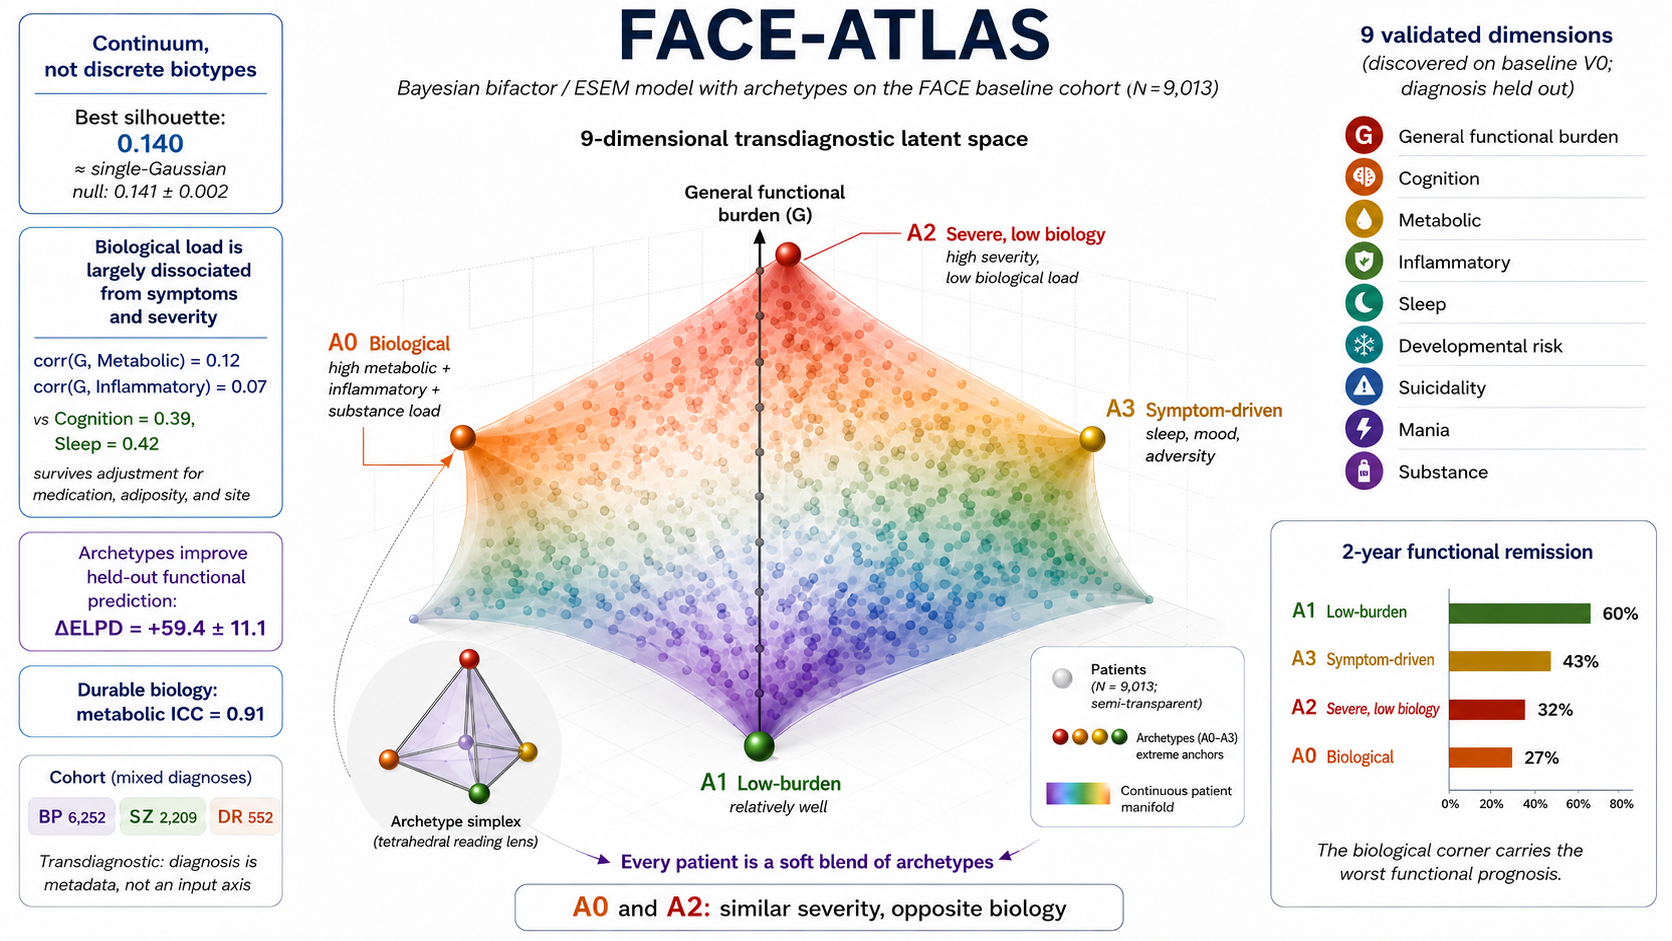
\includegraphics[width=\linewidth]{fig1_glance.png}%
  }{%
    \fbox{\parbox[c][6.6cm][c]{0.96\linewidth}{\centering\itshape
      Figure~1 (graphical abstract) renders here once the overview infographic is
      saved to \texttt{article/figures/fig1\_glance.png}.}}%
  }
  \caption{\textbf{A latent atlas of severe mental illness, at a glance.} The global,
  missingness-aware Bayesian bifactor / exploratory structural-equation model, fit to
  the FACE baseline ($N=9{,}013$) with diagnosis held out, yields a nine-dimension
  transdiagnostic latent space---a general functional-burden factor (\Gfac) and eight
  specific dimensions. The patient cloud is a graded continuum (best silhouette $0.140$,
  indistinguishable from a single-Gaussian null $0.141\pm0.002$), read through four
  archetypal extremes whose convex blends describe every patient: a \emph{biological}
  corner (A0; high metabolic, inflammatory and substance load), a \emph{low-burden} pole
  (A1), a \emph{severe, non-biological} corner (A2), and a \emph{symptom-driven} corner
  (A3). Metabolic and inflammatory load are largely dissociated from general burden
  (correlation $0.12$ and $0.07$, versus $0.39$ for cognition and $0.42$ for sleep, and
  robust to medication, adiposity and site); biology is durable (metabolic test--retest
  intraclass correlation $0.91$); the archetype phenotype improves held-out two-year
  functional prediction ($\Delta$ELPD $+59.4\pm11.1$); and two-year functional remission
  ranges $27\%$--$60\%$ across corners, the biological corner worst. A0 and A2 carry
  comparable severity but opposite biology.}
  \label{fig:glance}
\end{figure}

\subsection{A nine-dimension transdiagnostic map (the map exists)}

From ten candidate constructs, one global model returned a stable nine-dimension
structure: a general functional-burden factor (\Gfac) plus eight weakly correlated
specific axes---cognition, metabolic load, inflammation, sleep, developmental risk,
suicidality, mania and substance use (Figure~\ref{fig:atlas};
Table~\ref{tab:dimensions}). Inter-factor correlations among the specific axes were
weak throughout (mean absolute off-diagonal $\approx 0.10$), confirming genuinely
distinct axes rather than one collapsed dimension. \Gfac{} was anchored only by
functioning and global-severity indicators (FAST loading $0.90$, EGF $0.73$) and
carried no symptom content, supporting its conservative reading as transdiagnostic
\emph{functional burden} rather than a symptom-liability ``\textit{p}'' factor.
Depression and anxiety instruments (MADRS, QIDS, STAI) did not form a separate factor;
they loaded $0.66$--$0.80$ on \Gfac{} as cross-loading ``windows'' onto burden. The
single prior ``biology'' candidate \emph{split} into distinct metabolic and
inflammatory factors (inter-factor correlation $\approx 0.19$), and two constructs not
in the original ten---mania and substance use---were added once their indicators were
ingested and were confirmed in the joint fit. Of the candidates, nine were confirmed
(one as a split), anhedonia was rejected, and impulsivity, negative symptoms and
sensory abnormality were declared \emph{not testable} for lack of common
indicators---each verdict an outcome of the analysis rather than an assumption
(Table~\ref{tab:dimensions}). The structure was not an artefact of the priors: a
flat-prior refit reproduced the loadings and factor correlations essentially exactly
(Tucker congruence $\varphi = 1.00$), and model comparison decisively preferred the
bifactor over unidimensional and correlated-factor alternatives. Absolute fit was
acceptable across both likelihood blocks (continuous Bayesian standardized
root-mean-square residual $\approx 0.07$; $21/22$ non-Gaussian indicators reproduced
within the $90\%$ posterior-predictive interval).

\begin{figure}[t]
  \centering
  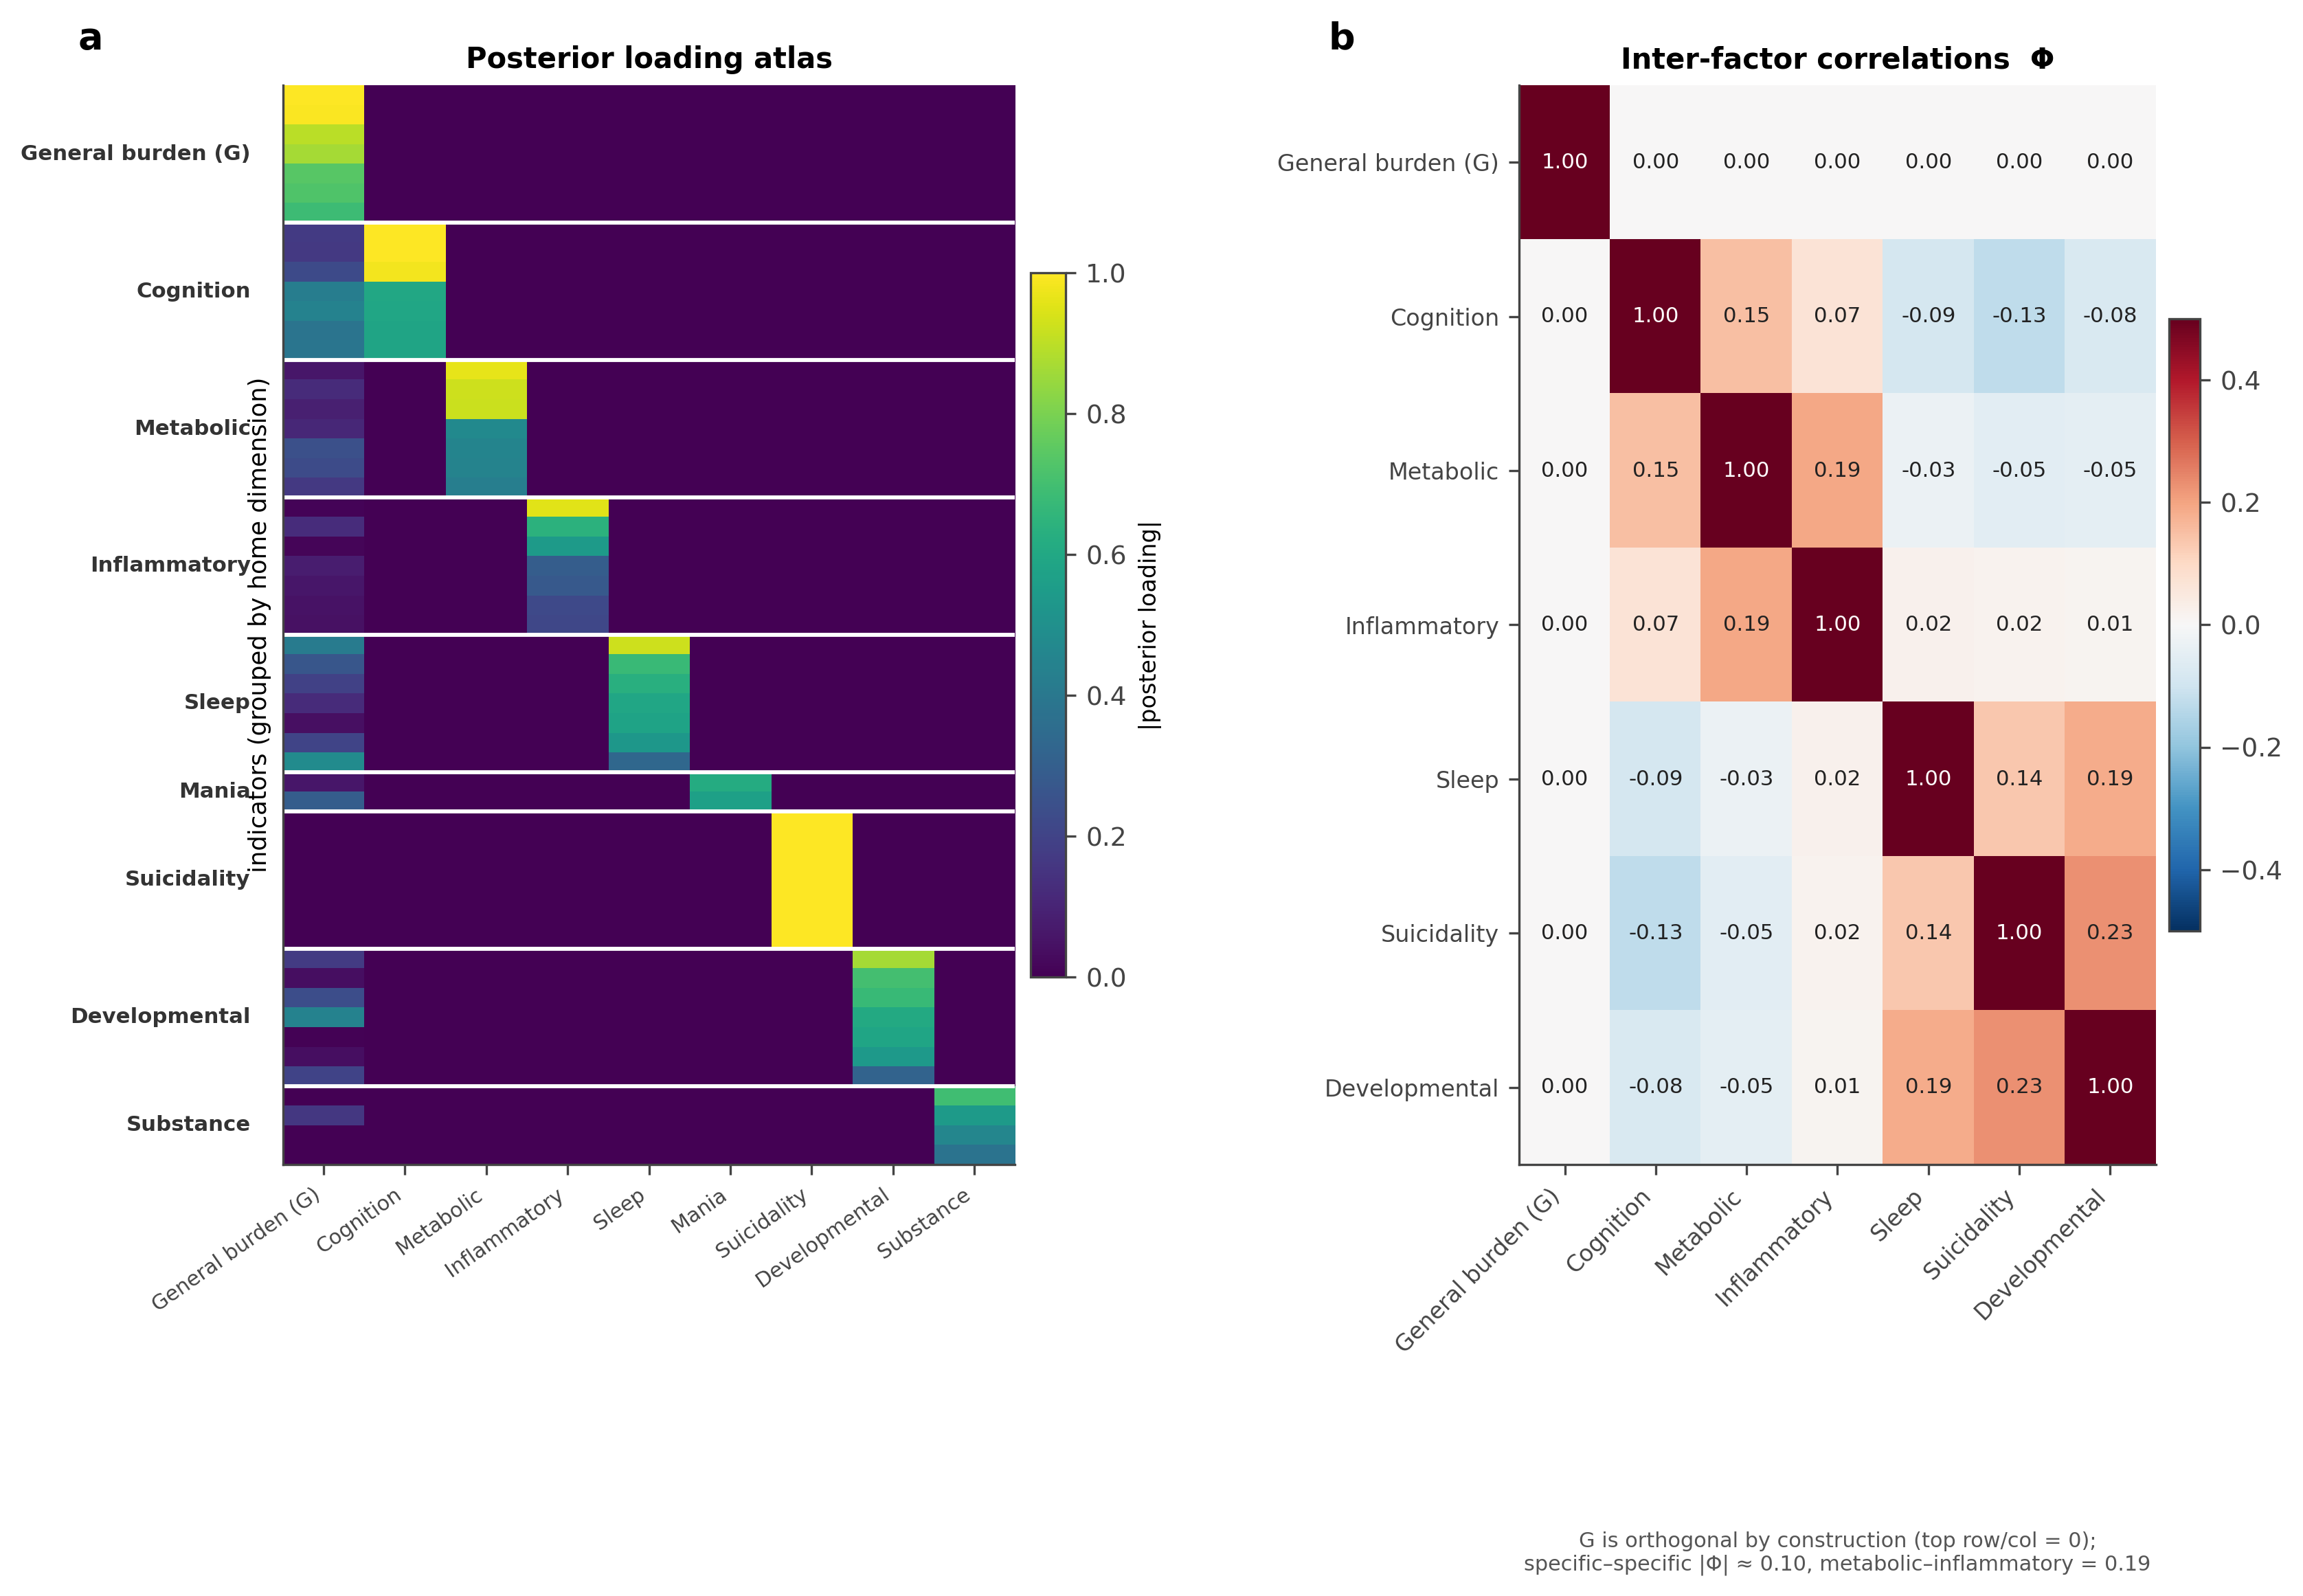
\includegraphics[width=0.98\linewidth]{fig2_map.png}
  \caption{\textbf{The nine-dimension map.} (\textbf{a}) Posterior loading atlas
  (indicators $\times$ factors); colour encodes the absolute posterior loading, with
  rows grouped by home factor. Each specific axis is anchored by a clinically coherent
  indicator block, while \Gfac{} (functional burden) carries the cross-loading
  depression/anxiety windows. (\textbf{b}) The inter-factor correlation matrix is weak
  throughout (mean $|\text{off-diagonal}|\approx 0.10$); the general factor is
  orthogonal to the specific axes by construction (top row and column), and metabolic
  and inflammatory load correlate only $\approx 0.19$. Continuous backbone shown;
  mania and substance enter the joint mixed fit (Table~\ref{tab:dimensions}).}
  \label{fig:atlas}
\end{figure}

\subsection{Biology is the least severity-entangled domain (the central finding)}

Because the bifactor identification fixes \Gfac{}~\orth{}~specifics by construction,
we re-estimated the model allowing \Gfac{} to correlate freely with the specific axes.
Under this correlated-\Gfac{} model, metabolic and inflammatory load were the
\emph{least} entangled with functional burden: correlations with \Gfac{} of $0.12$
(metabolic) and $0.07$ (inflammatory), against $0.39$ for cognition and $0.42$ for
sleep (Figure~\ref{fig:biologyg}). Two patients with the same overall impairment can
therefore carry very different metabolic and immune loads: a patient's biological
burden rides largely on axes that the global clinical-severity picture does not
capture. This dissociation was robust to the obvious confounders. Adjusting each
indicator for age, sex, education and recruitment site, and then additionally for
antipsychotic exposure, did \emph{not} raise the biological correlations---if anything
it lowered them (metabolic $0.12\!\to\!0.07$, inflammatory $0.07\!\to\!0.06$), and the
biological axes remained the least entangled at every step
(Figure~\ref{fig:biologyg}; Annex~\ref{ann:measurement}). Consistent with a large
independent literature (Discussion), we state this as relative, not absolute,
independence: metabolic and inflammatory load are \emph{largely independent of a
general functional-burden axis}, with the $0.07$--$0.12$ values quantifying---at the
low end of what that literature would predict---a pattern previously described only
qualitatively. This is the property a biology-aware stratification can exploit, and it
is the load-bearing premise of everything that follows.

\begin{figure}[t]
  \centering
  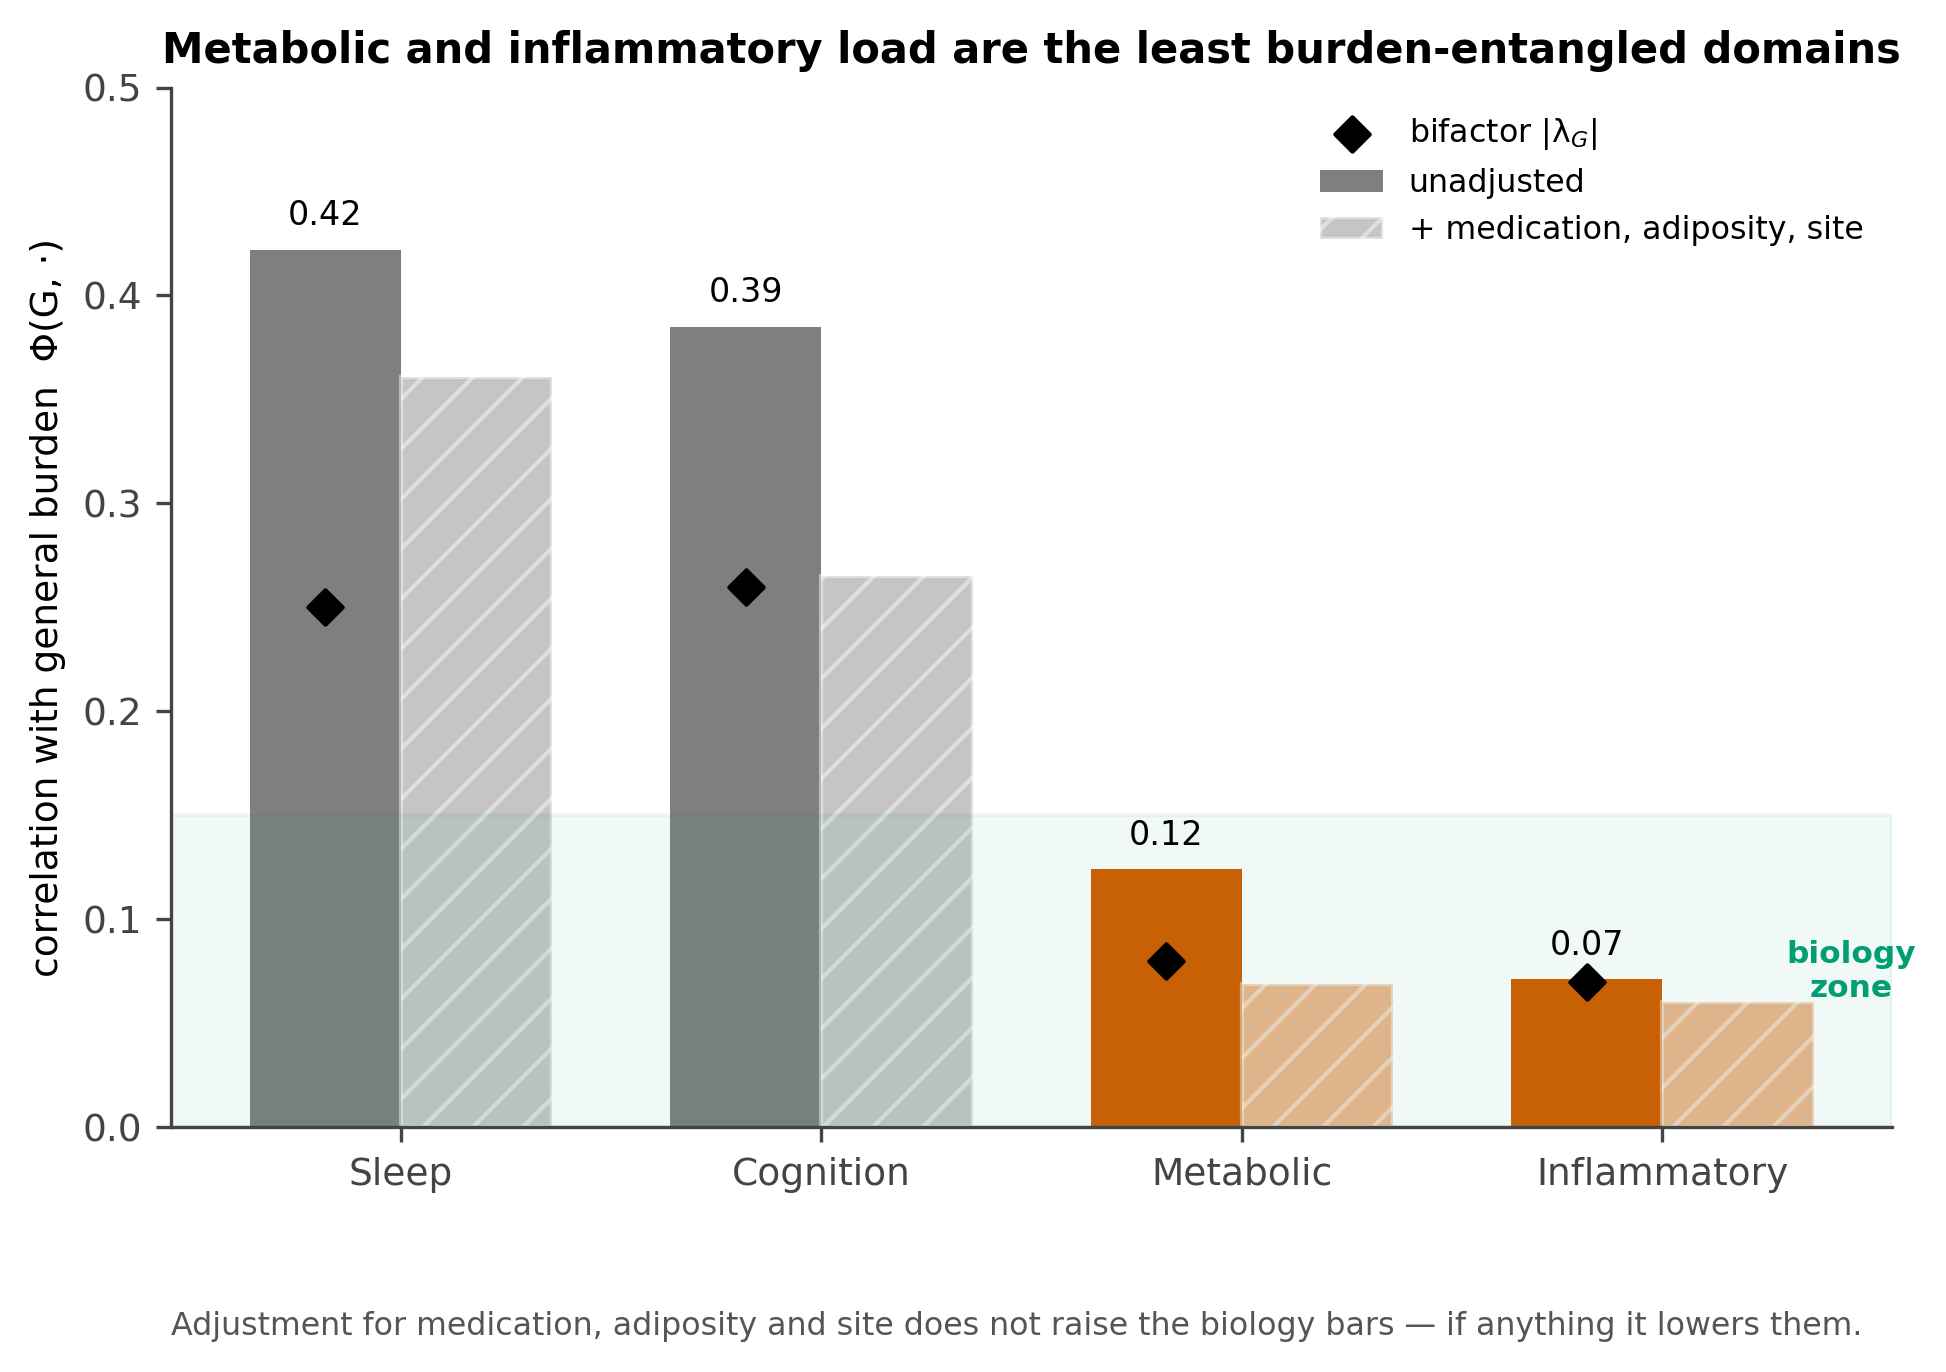
\includegraphics[width=0.80\linewidth]{fig3_biology_g.png}
  \caption{\textbf{Metabolic and inflammatory load are the least burden-entangled
  domains.} Correlation of each continuous specific axis with the general
  functional-burden factor \Gfac{} (bars), unadjusted and after adjustment for
  medication, adiposity and site; the bifactor general loading $|\lambda_G|$
  (diamonds) is shown for comparison. Metabolic and inflammatory load fall in the
  ``biology zone'' ($\Phi<0.15$) and stay there under adjustment, whereas cognition
  and sleep partly track \Gfac{}.}
  \label{fig:biologyg}
\end{figure}

\subsection{The patient space is a continuum, not biotypes (the map organizes)}

On these nine coordinates, with each patient's measurement uncertainty propagated, the
patient space is a graded continuum rather than a set of discrete biological kinds. A
structure-discovery battery run over the posterior draws---cluster tendency, modality,
silhouette, the gap statistic, a Gaussian-mixture information criterion, density-based
clustering and a topological summary---returned a continuum verdict: the silhouette
peaked at only $0.14$ (below the $0.15$ separation floor), the first principal
component was unimodal (Hartigan dip $p\approx 1.0$), density-based clustering assigned
$100\%$ of points to noise, and the topological summary was a single connected
component. A single-Gaussian \emph{falsification null} made the verdict decisive: the
best partition of the real cloud separated patients no better than slicing a
structureless Gaussian blob of identical covariance (best silhouette $0.140$ for the
real data versus $0.141\pm0.002$ for the null, $z=-0.36$; the Gaussian-mixture-optimal
number of components collapsed to one in all $20$ posterior draws;
Figure~\ref{fig:continuum}a). There are, in this clinical--biological space, no
well-separated, reproducible discrete clusters.

We therefore represent the space by its geometry rather than by a partition. Diagnosis
is intermixed throughout the cloud (Figure~\ref{fig:continuum}b); overall burden forms
a smooth gradient along the principal axis (Figure~\ref{fig:continuum}c); and
inflammatory load varies along a \emph{different} direction
(Figure~\ref{fig:continuum}d)---the biology\,\orth\,\Gfac{} dissociation, made visible.
Four archetypal extremes, selected by cross-seed stability rather than by a
parsimony rule (the only stable resolutions were two and four corners; cross-seed
Tucker congruence $0.98$), give the continuum a clinically legible reading
(Figure~\ref{fig:continuum}e). They separate biology from symptoms from severity: a
\emph{biological} corner (high metabolic, inflammatory and substance load), a
\emph{low-burden} pole, a \emph{severe, non-biological} corner (high overall severity
but low biological load), and a \emph{symptom} corner (high sleep, developmental,
suicidality and mania). Each patient is a soft convex blend of all four (mean
assignment entropy $0.78$); only $39\%$ sit near a single pole. The reading is
transdiagnostic (adjusted Rand index $\approx 0$ against both cohort and the seven
DSM-5 subtypes), driven by the specific and biological axes rather than by severity
(variance explained by the coarsest tessellation: specific axes $\eta^2=0.12$ versus
$\Gfac{}$ $0.008$), not a missingness artefact (a classifier predicting region
membership from each patient's coverage pattern performed below baseline, lift
$-0.05$), and a tighter description of the coordinate cloud than diagnosis
(mixture information criterion $197{,}900$ versus $201{,}300$ for a DSM-5-constrained
model). Critically, because biological load varies continuously without a density
\emph{gap}, it never forms a clean partition boundary at any granularity; it surfaces
instead as an archetypal \emph{corner}. The biological phenotype is thus a direction
in a continuum, not a category---which is exactly why the continuous coordinates and
the archetype simplex, not any hard tessellation, are the load-bearing objects
downstream.

\begin{figure}[t]
  \centering
  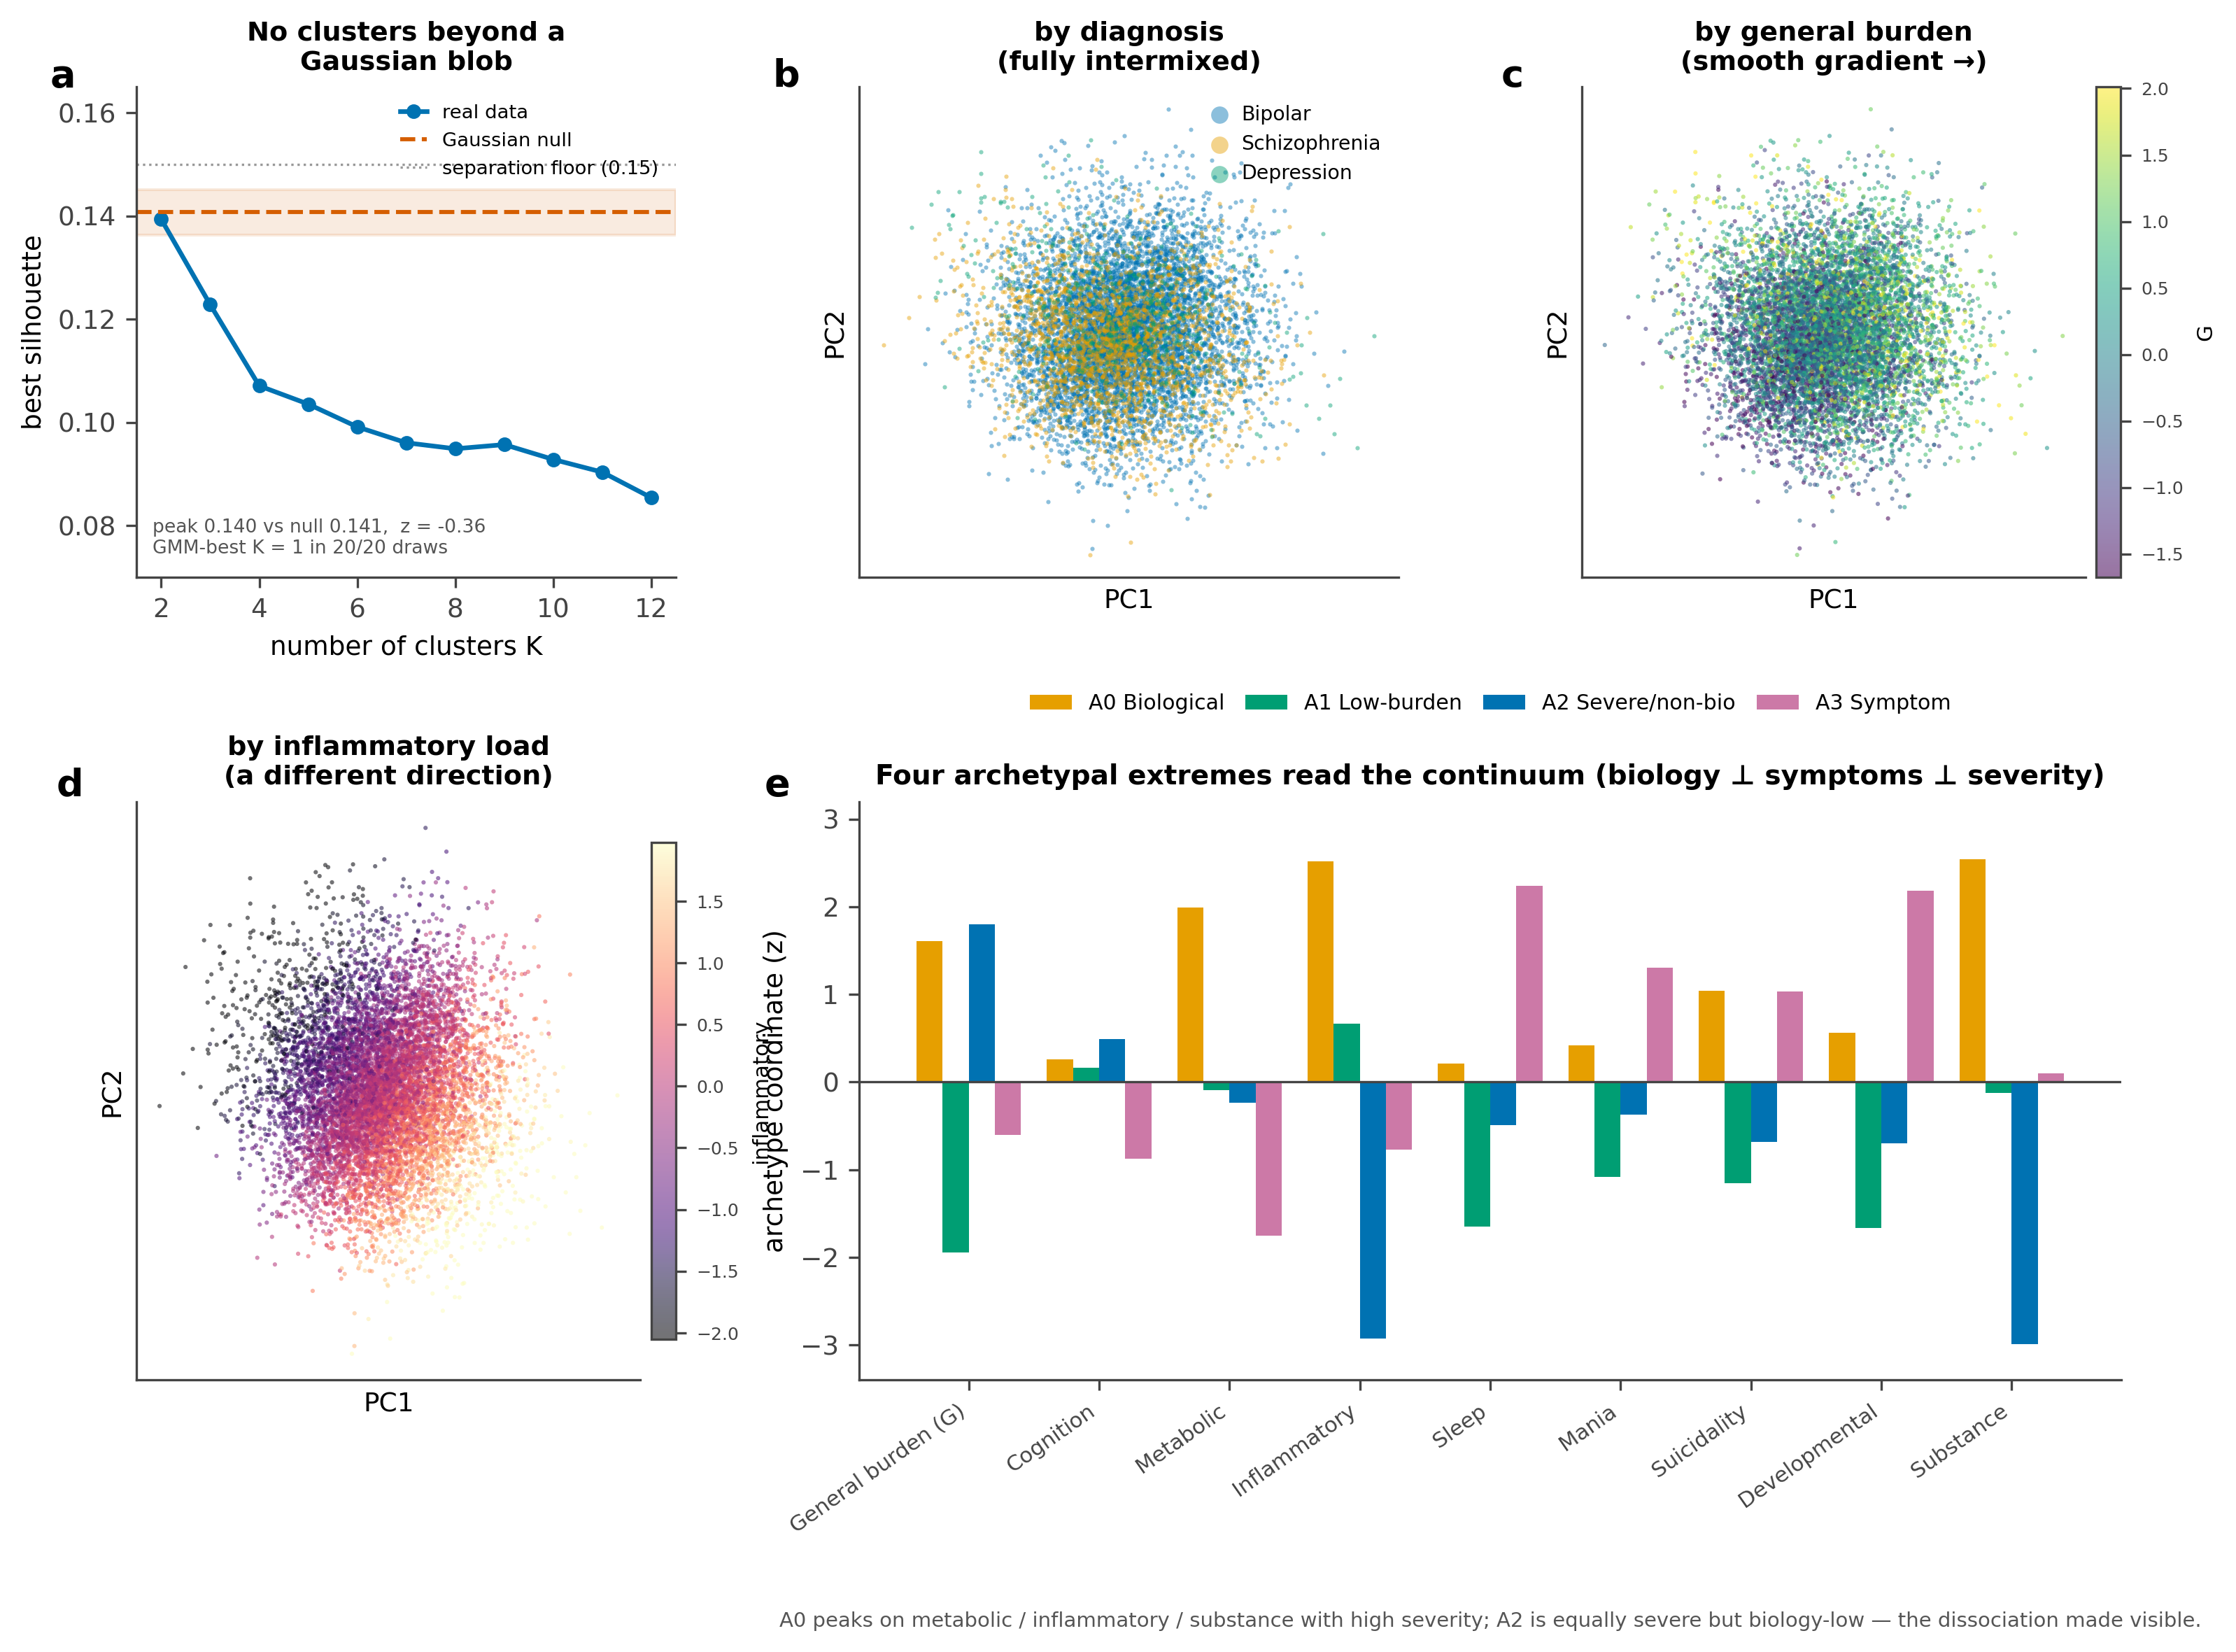
\includegraphics[width=0.99\linewidth]{fig4_continuum.png}
  \caption{\textbf{The patient space is a continuum, not biotypes.} (\textbf{a}) A
  single-Gaussian falsification null: the best silhouette achievable on the real
  nine-dimensional cloud is no better than on a structureless Gaussian of matched
  covariance ($z=-0.36$); the mixture-optimal number of clusters is one in all
  posterior draws. (\textbf{b--d}) Principal-component embedding of the coordinates
  ($N=9{,}013$), coloured by diagnosis (fully intermixed), by general burden \Gfac{}
  (a smooth gradient), and by inflammatory load (a gradient in a \emph{different}
  direction). (\textbf{e}) Standardized profiles of the four archetypal extremes
  across the nine axes; the biological corner (A0) and the severe, non-biological
  corner (A2) carry comparable general burden but opposite biological profiles.}
  \label{fig:continuum}
\end{figure}

\subsection{The geometry persists over two years (the map persists)}

Scored forward onto the $12$- and $24$-month visits on the \emph{fixed} model
(observed cells, uncertainty propagated, never re-estimated; baseline coordinates
reproduced at Pearson $r\approx0.99$ through this path), the measurement remained
invariant for all five testable backbone axes (longitudinal Tucker congruence
$\varphi = 0.97$--$1.00$; inflammatory load, only partially invariant on a plain
Gaussian map, was invariant here at $\varphi=0.97$; \edfig{fig:invariance}). Coordinate
change can therefore be read as patient change rather than instrument drift. A
measurement-error decomposition then separated trait from state
(Figure~\ref{fig:traitstate}). The durable, trait-like axes were the biological and
cognitive ones (test--retest intraclass correlation: metabolic $0.91$, substance
$0.88$, cognition $0.70$, inflammatory $0.62$); the moving, state-like axes were the
symptom ones (sleep $0.47$, suicidality $0.42$, developmental risk $0.39$). General
burden was trait \emph{by rank} (intraclass correlation $0.62$): patients largely kept
their relative position even as the cohort as a whole improved on severity and symptoms
(population shift $-0.46$ on \Gfac{} and $-0.84$ on suicidality, while biology stayed
static). Archetype identity persisted---the archetype weight vector moved little over
two years (median cosine similarity $0.90$). The clinical reading is compact:
\emph{stratify on the durable biology; monitor the moving symptoms}.

\begin{figure}[t]
  \centering
  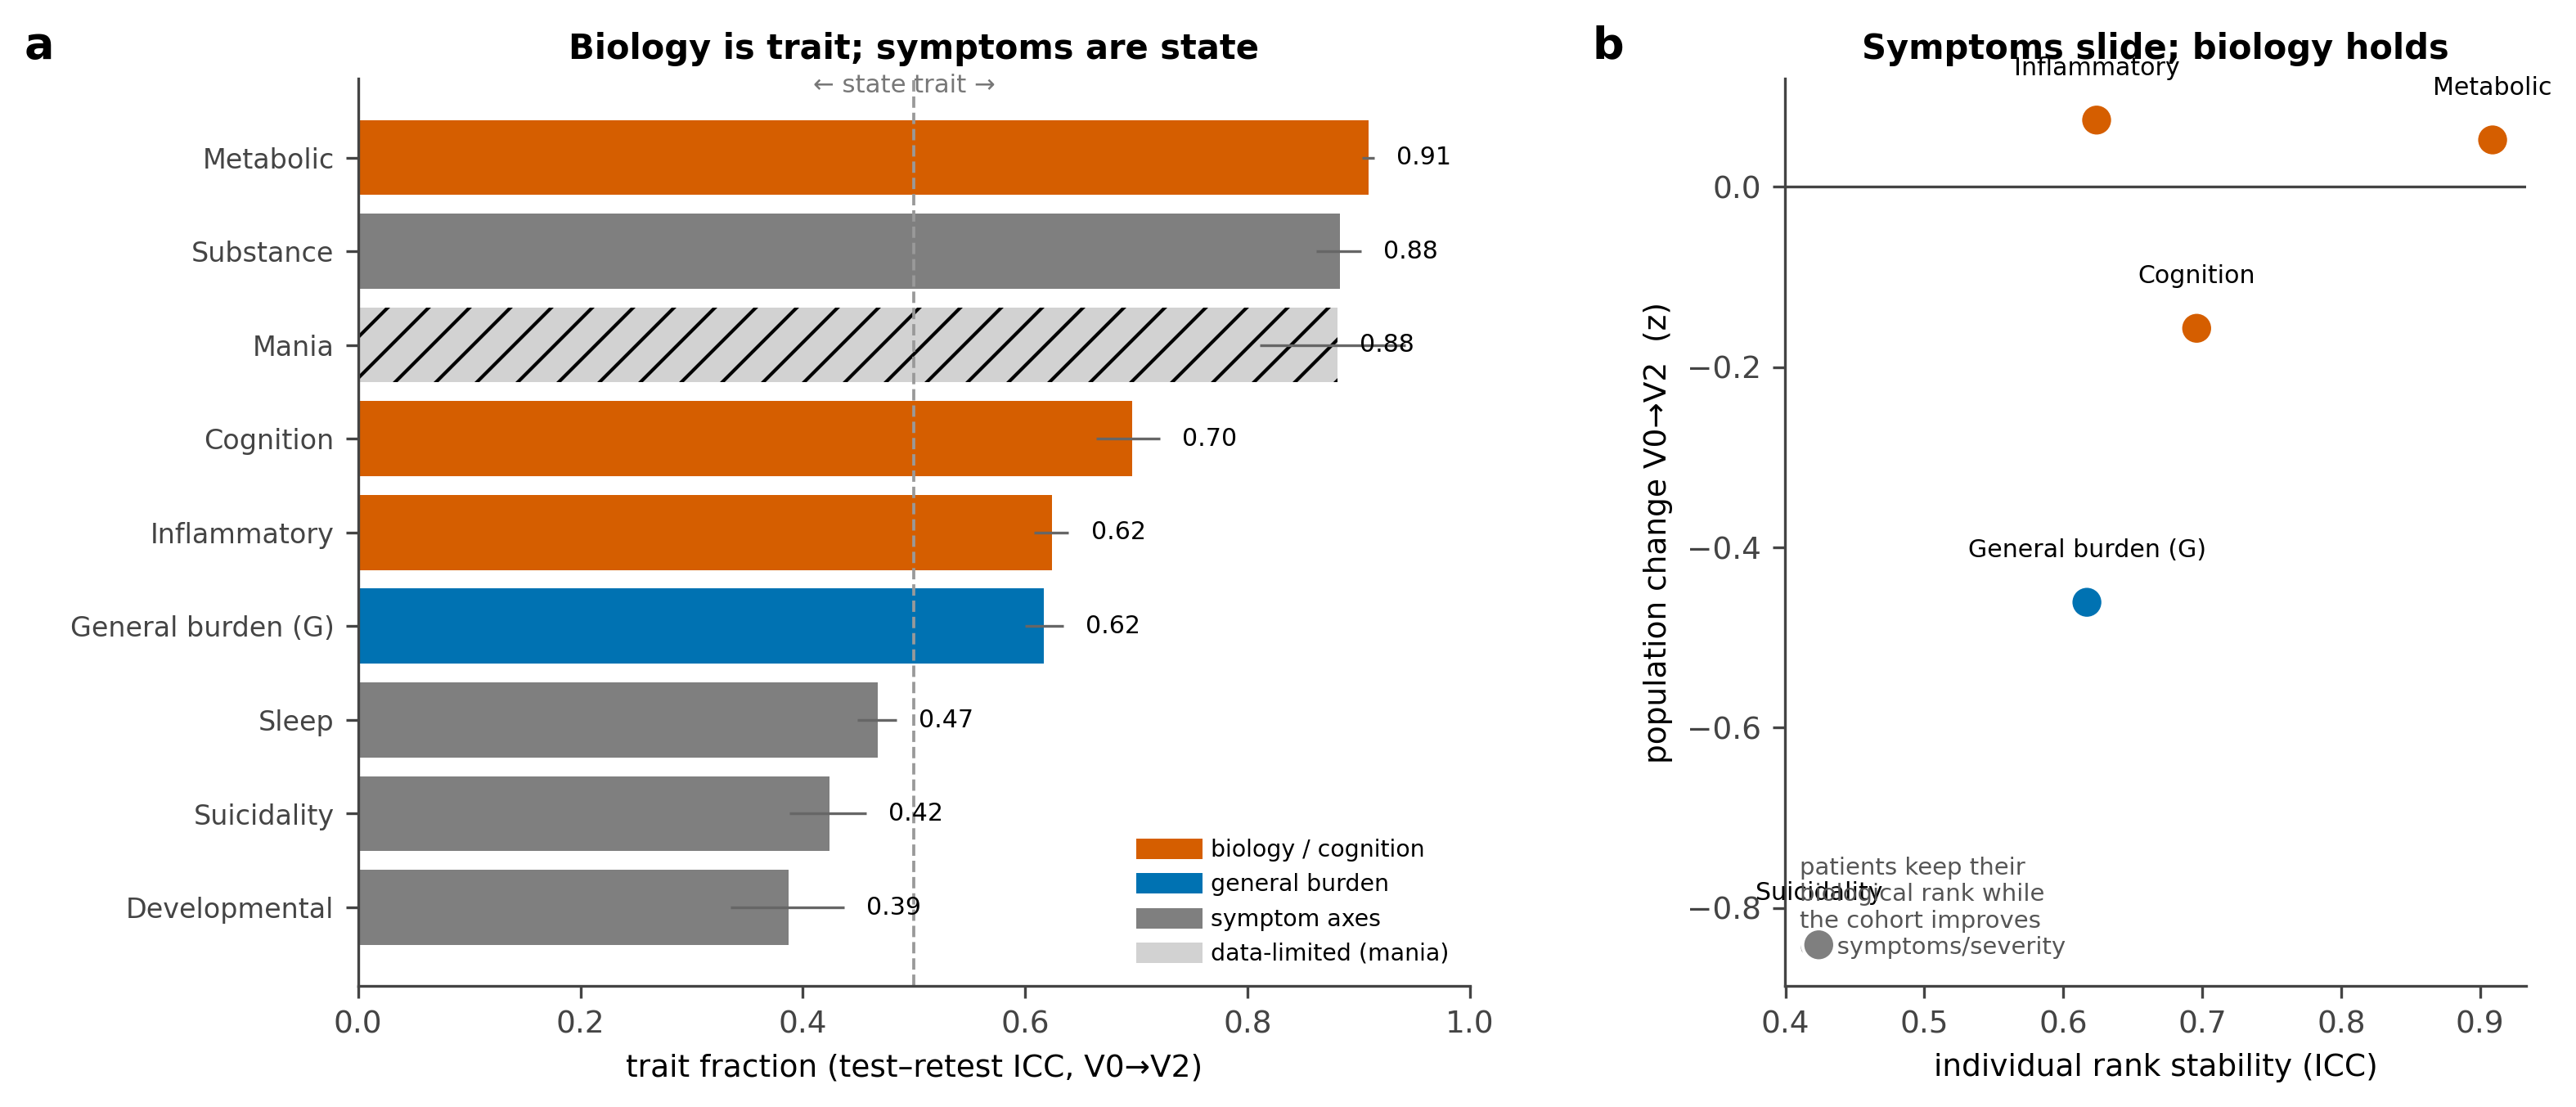
\includegraphics[width=0.98\linewidth]{fig5_persistence.png}
  \caption{\textbf{Durable biology, moving symptoms.} (\textbf{a}) Trait fraction
  (test--retest intraclass correlation, with $94\%$ credible intervals) over
  follow-up: the biological and cognitive axes are trait-like, the symptom axes
  state-like; mania is data-limited (hatched). (\textbf{b}) Individual rank stability
  versus population-level change: patients keep their biological rank (high intraclass
  correlation, near-zero population shift) while the cohort slides down the severity
  and symptom axes.}
  \label{fig:traitstate}
\end{figure}

\subsection{It predicts future functioning, modestly and at the group level (the map predicts)}

We then asked whether a baseline coordinate or phenotype predicts a two-year outcome
\emph{incrementally beyond} diagnosis, current severity and the baseline value of the
outcome, using an errors-in-variables Bayesian model that propagated each coordinate's
measurement uncertainty. The map added predictive signal for \emph{functioning} but
not for severity (which was saturated by its own baseline autoregression). The signal
was carried by the \emph{phenotype}, not by any single laboratory axis: the four
archetypes added the most held-out predictive value (expected log predictive density
gain $+59$ over the diagnosis-plus-severity-plus-baseline reference), the eight
specific axes added $+37$, and---an honest, map-specific shift from our earlier
analyses---the isolated ``durable biology'' axes \emph{alone} no longer cleared the
bar ($+2$, ambiguous; Figure~\ref{fig:prognosis}b). Biology still predicts functioning,
but as a \emph{corner of the phenotype} (the biological archetype) rather than as a
standalone three-axis block. No hard partition improved on the continuous and
archetype encodings (every tessellation added $\approx+20$, strictly dominated by the
archetypes); the operative number of clusters is therefore \emph{none}---the actionable
object is a continuous position, not a category. The map was \emph{co-informative} with
DSM-5 rather than redundant with it (functioning: map $+22$, DSM-5 $+29$, both $+67$;
Figure~\ref{fig:prognosis}c), and \emph{course-dependent}, with the signal concentrated
in the episodic, open-course cohorts (bipolar disorder and depression) and weak when
bipolar disorder was removed.

Translated to the clinic, the four archetypes sorted patients into groups whose
two-year functional-remission rate ranged from $27\%$ to $60\%$, transdiagnostically
(Figure~\ref{fig:prognosis}a); the \emph{biological} corner carried the worst
functional prognosis ($27\%$), worse than the equally severe non-biological corner
($32\%$)---the dissociation translating into prognosis. This gradient was a genuine
within-diagnosis effect, not a cohort-composition artefact: the rank held inside every
cohort (a biological-vs-low-burden odds ratio $\approx 4$ in each), standardizing to a
common cohort mix moved it by only $\approx 6\%$, and the corner-by-cohort interaction
was non-significant. The individual-level discrimination gain was nonetheless small
(functional-remission AUC $+0.011$ over a strong diagnosis-plus-severity reference):
the map's value is group-level prognostic stratification and continuous functional
forecasting, not a large boost to individual binary prediction. The functioning signal
survived inverse-probability weighting for attrition ($+53$), restriction to either
two of the three cohorts ($+56$, $+59$), and a permutation null (which correctly
vanished). Finally, against the full set of $143$ raw indicators under a matched
gradient-boosting classifier, the nine-dimension map was a \emph{sufficient}
representation for predicting deterioration (equal AUC) and \emph{near-sufficient} for
recovery (raw indicators $+0.04$ AUC), with $97\%$ of the raw recovery signal already
contained within the nine factors (\edfig{fig:repbench})---the compression is faithful,
not lossy in any axis the map omits.

\begin{figure}[t]
  \centering
  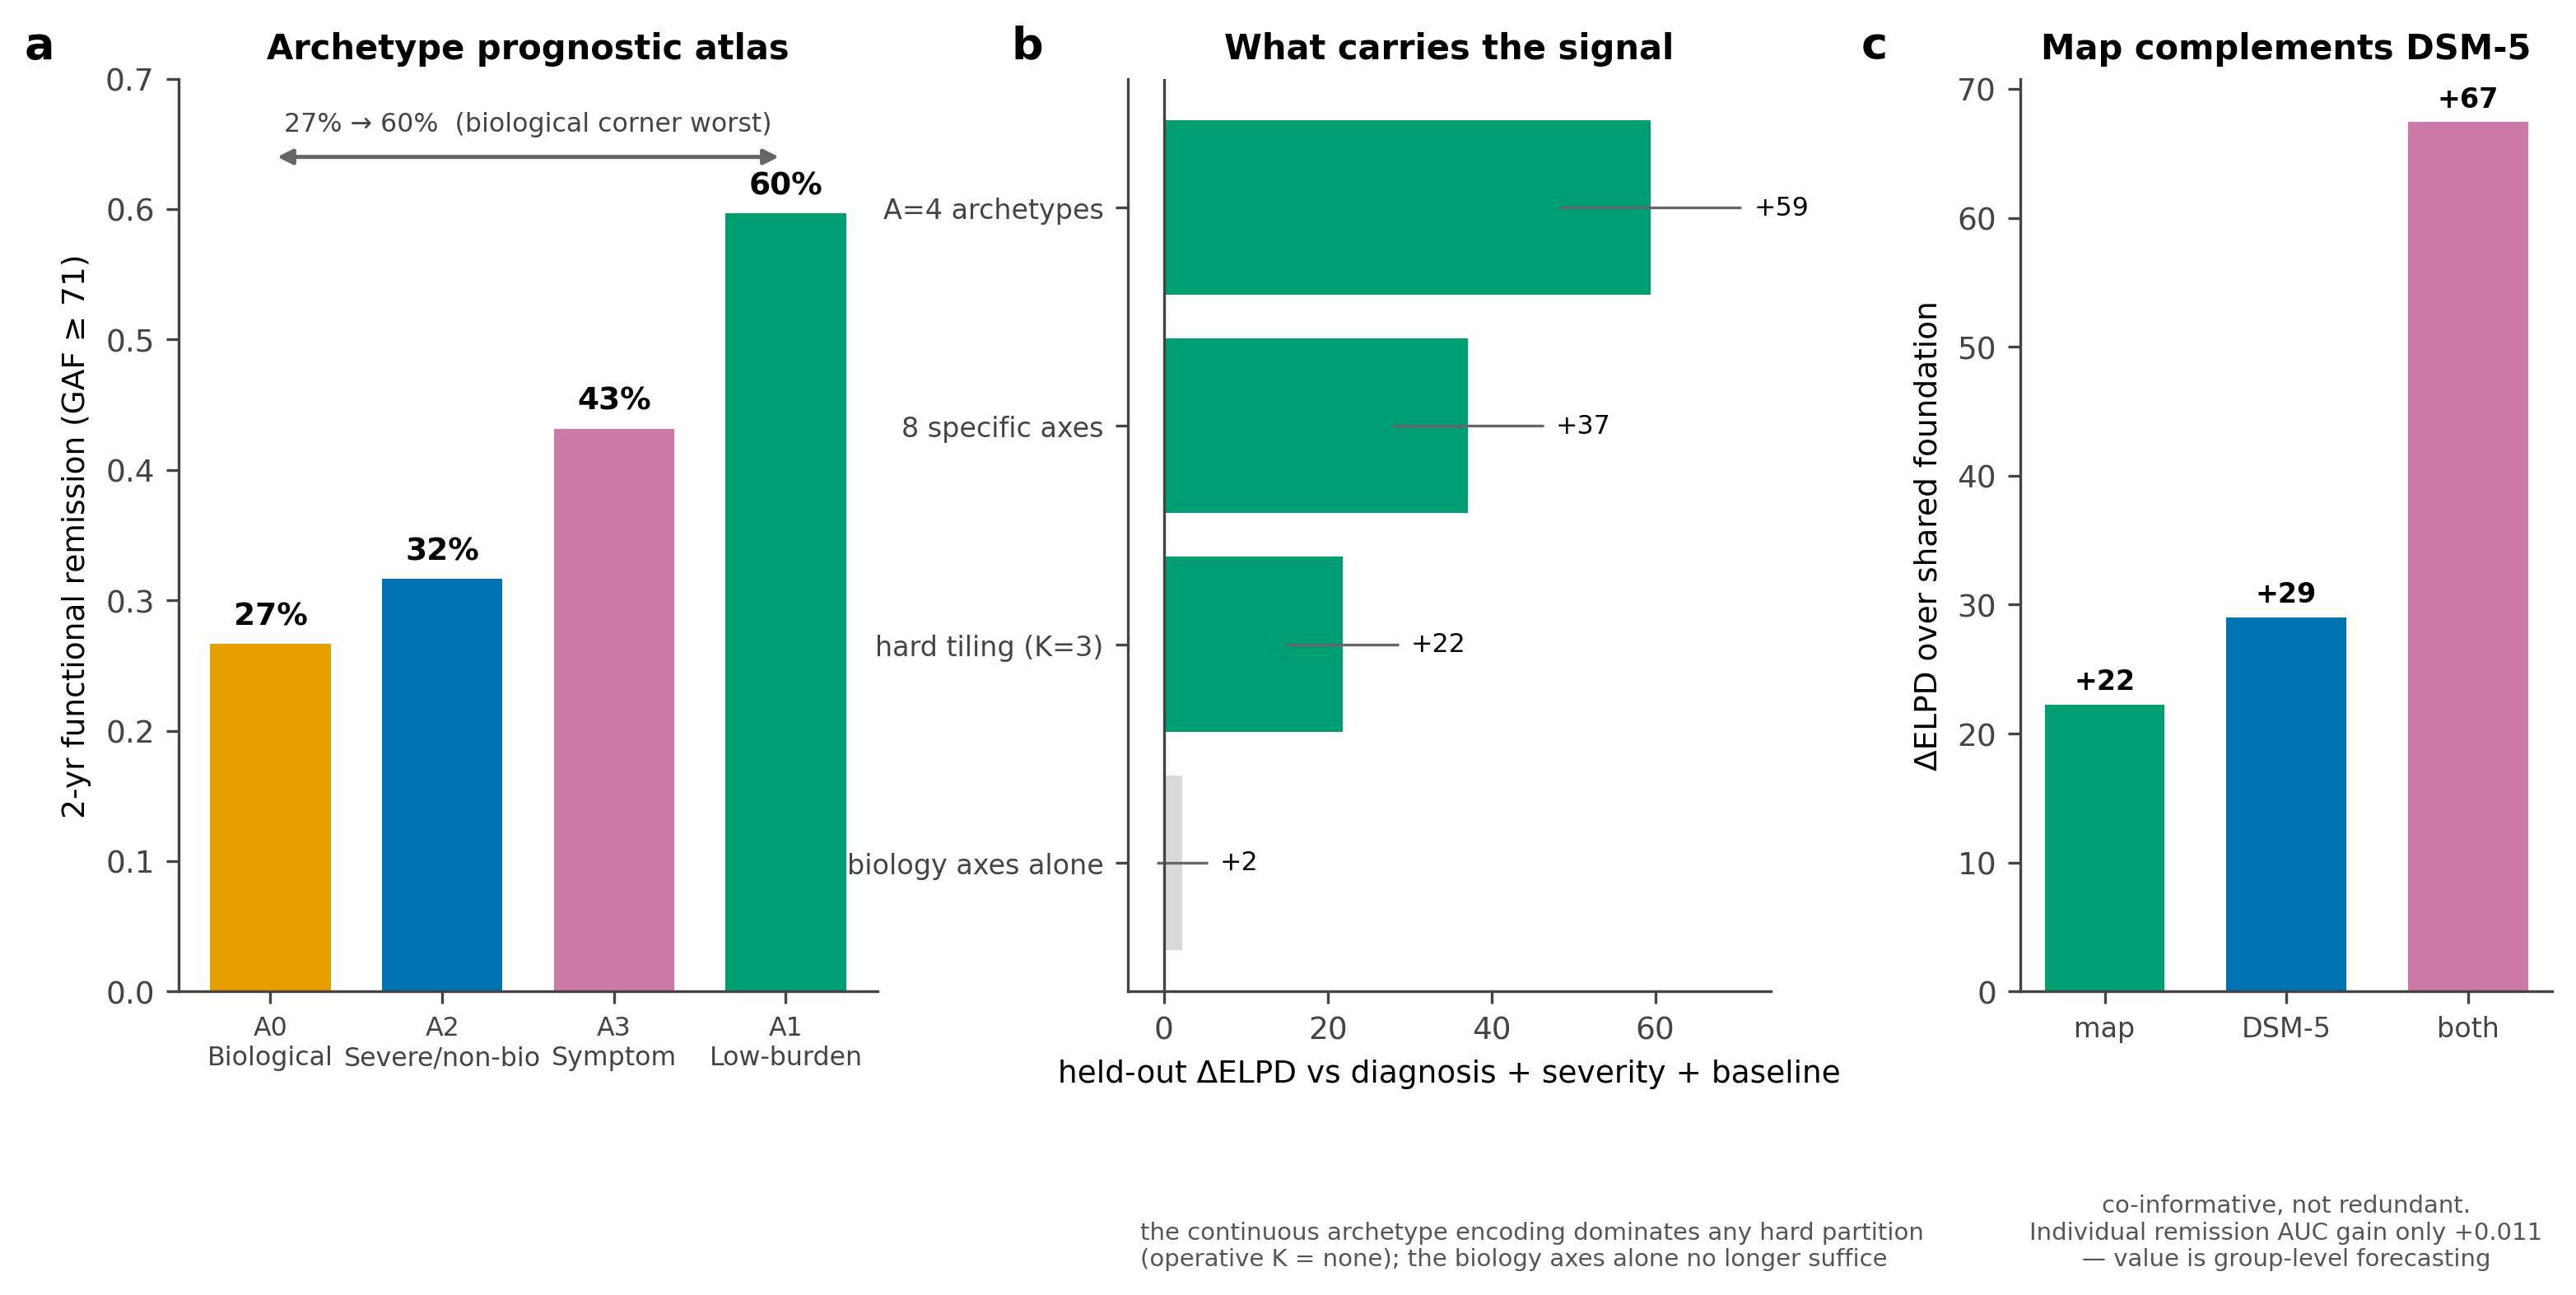
\includegraphics[width=0.99\linewidth]{fig6_prognosis.png}
  \caption{\textbf{Prognostic reach for functioning.} (\textbf{a}) Archetype
  prognostic atlas: two-year functional-remission rate by baseline archetype; the
  biological corner is worst ($27\%$) and the low-burden pole best ($60\%$), a
  transdiagnostic $27\%$--$60\%$ gradient. (\textbf{b}) Held-out incremental value for
  functioning: the continuous archetype encoding dominates the eight specific axes, any
  hard tessellation, and the isolated biology axes (operative number of clusters
  $=$ none). (\textbf{c}) The map and DSM-5 are co-informative---each adds beyond the
  other, and both together add most---but the individual-level remission AUC gain is
  only $+0.011$.}
  \label{fig:prognosis}
\end{figure}

\subsection{It does not yet guide treatment---a boundary drawn by the evidence}

Treatment exposures, recovered from the per-cohort source dictionaries and harmonized
to drug-class indicators, were run through an identification-first causal pipeline
(common-support overlap gate $\rightarrow$ propensity weighting $\rightarrow$
doubly-robust errors-in-variables moderation with an E-value sensitivity analysis and a
minimum-detectable-effect calculation) to ask whether the durable axes or the
archetypes \emph{moderate} treatment response. On observational, expert-centre
treatment-as-usual they did not reliably do so (\edfig{fig:treatment}a). Where
identification was cleanest---lithium in bipolar disorder, near-complete overlap---the
result was a \emph{well-identified, bounded null}: the average effect was
indistinguishable from zero (E-value $1.06$) and the design could have resolved an
interaction as small as $\approx 0.2$ standard deviations but did not. An
antipsychotic-by-biology signal for functioning in bipolar disorder was a confounded
\emph{average} effect (E-value $1.77$) with \emph{no} reliable moderation (the two map
encodings disagreed on which axis carried it---the signature of a false positive); and
clozapine in schizophrenia was channelled to treatment-resistant patients and hence
underpowered rather than cleanly null. Average treatment effects were uniformly
confounding-fragile (E-values $1.1$--$1.8$), the expected signature of confounding by
indication.

This boundary is earned, not assumed, and it cuts two ways that strengthen the rest of
the paper. First, the prognostic finding was \emph{not} merely unmodelled treatment:
the archetype carrier of the functioning forecast survived adjustment for the drug
classes patients were actually receiving (attenuation $4.7\%$; $3.9\%$ under attrition
weighting), so the biological phenotype is not a treatment proxy. Second, even without
\emph{selecting} a drug, the map \emph{describes} who faces a difficult course: the
baseline archetype stratified two-year treatment course, with the biological corner
carrying roughly twice the treatment-resistance and side-effect burden of the
low-burden corner (resistance $43\%$ vs $20\%$; significant side-effects $23\%$ vs
$11\%$), beyond baseline severity, substance comorbidity and demographics, and within
cohort (\edfig{fig:treatment}b). As in the prognostic analysis, this is a group-level
monitoring signal, not an individual classifier (the steepest gradient,
treatment-resistance, was AUC-marginal under a permutation null). Demonstrating
treatment \emph{selection} from this map would require randomized or trial-arm data,
which this baseline observational cohort---patients receiving usual care in French
expert centres---does not contain.

\section{Discussion}

Across three cohorts of severe mental illness, a single missingness-aware Bayesian
model places clinical and biological measurements in one transdiagnostic coordinate
system and yields an eight-dimension atlas whose most consequential property is a
dissociation: immunometabolic load is the domain least entangled with overall
functional severity. The cardiometabolic and inflammatory markers resolve as a single
immunometabolic axis anchored by body composition (BMI loading $\approx 0.95$, weight
$0.88$, waist circumference $0.84$), with smaller metabolic, inflammatory and
cardiovascular contributions (C-reactive protein $\approx 0.37$); that axis sits nearly
independent of \Gfac{}. Because the one inflammatory marker available here, CRP, is itself
substantially adiposity-driven~\citep{kappelmann2021,norton2025crp}, we read this as an
adiposity-anchored cardiometabolic axis and do not interpret it as an inflammatory
dimension independent of body composition---the IL-6-type signal implicated in mood
pathology~\citep{ye2021inflammation,milaneschi2021} was not measured here. The axis is
nonetheless more than body habitus: excluding the anthropometric indicators and refitting,
a coherent cardiometabolic--inflammatory axis survived, highly congruent with the full axis
(Tucker $\varphi=0.90$; Supplement~\ref{annA:nobmi}). If biological burden simply tracked how impaired a
patient is, it would add little to a clinician's global impression. The data say the
opposite---biological risk rides on an axis the severity picture does not see---and the
five archetypal extremes make the consequence concrete. The immunometabolic corner and
the severe, clean-biology corner carry comparable functional burden but opposite
biological profiles, and they diverge in prognosis (the immunometabolic corner is the
worst-prognosis pole and the well pole the best, two-year functional remission spanning
$17\%$ to $52\%$ across the five corners). This is the precise property a
biology-aware stratification can exploit: it separates patients who look equally ill
but are biologically opposite, and that separation is durable and prognostically
meaningful.

This headline is corroborated, in direction, by a large and independent literature,
which is why we state it as relative rather than absolute independence. Metabolic
burden in severe mental illness is driven by medication, adiposity, age and chronicity
more than by diagnosis or symptom severity, is present before chronic severity
accrues, and is comparable across schizophrenia, bipolar disorder and
depression~\citep{vancampfort2015mets,vancampfort2016diabetes,pillinger2017,perry2019,garridotorres2022};
inflammation marks a subgroup and specific symptoms rather than the severity
continuum~\citep{osimo2019,fernandes2016bd,fernandes2016sz}; and the
immuno-metabolic-depression programme has independently arrived at a separable
biological dimension mapping onto atypical, energy-related
symptoms~\citep{penninx2024imd,milaneschi2020,lamers2013,lamers2020,milaneschi2017}.
That a completely different method, in different cohorts, converges on a separable
biology axis is strong convergent validity. We also state the boundary conditions
plainly: case--control inflammatory elevations are
real~\citep{howren2009,osimo2020,haapakoski2015}, a modest severity or duration
dose--response for metabolic burden exists~\citep{penninxlange2018,pillinger2022},
metabolic dysfunction does track cognition and functioning in mood
disorders~\citep{maksyutynska2024}, and much of the inflammation--symptom association
is carried by adiposity rather than inflammation \emph{per
se}~\citep{kappelmann2021,zagaria2024}. Our small immunometabolic--\Gfac{} couplings
are best read as a quantification of a known qualitative pattern, sitting at its low
end because \Gfac{} indexes \emph{functional burden}---from which biology is most
decoupled---rather than the case--control contrast of being ill. That they survive,
and even fall slightly under, adjustment for medication, adiposity and site is the
strongest available evidence that the dissociation is not a confound.

The second contribution is structural. On these clinical--biological coordinates the
patient space is a graded continuum, not a set of discrete biotypes, and it cuts
almost entirely across DSM-5. This aligns with normative-modelling work reporting
extensive individual heterogeneity in the same
disorders~\citep{wolfers2018,marquand2016,segal2023}, and it stands in apparent
tension with the brain-based B-SNIP biotypes~\citep{clementz2016biotypes,clementz2020}.
The tension is more apparent than real: the two programmes interrogate different
measurement spaces, B-SNIP itself found DSM diagnoses to be a severity continuum, and
recent syntheses endorse both categorical and dimensional
views~\citep{clementz2024}; clustering choices can also resurface apparent biotypes
from continuous data~\citep{pan2026}. We therefore claim no biotypes \emph{in this
eight-dimensional clinical--biological space}---a claim we make rigorous with a
single-Gaussian falsification null (best-partition silhouette $0.140$ against a
structureless-Gaussian null of $0.137 \pm 0.002$, $z = 1.13$) rather than by the
absence of an elbow---not that biotypes are absent from all spaces. The five
archetypes are corners of this continuum, not clusters within it, and the partition
they induce is driven by activation and suicidality rather than by overall severity,
which is why it cuts almost orthogonally across DSM-5 (ARI $0.006$) while describing
the space more tightly than diagnosis does. Anchoring \Gfac{} on functioning alone also
sidesteps the well-known instability in what a symptom-only general factor
means~\citep{heinrich2021bifactor,levinaspenson2020,watts2021}, while remaining
consistent with the impairment reading of the \textit{p}
factor~\citep{caspi2014pfactor,lahey2017general}.

The remaining contributions are deliberately calibrated. The map persists over two
years---durable biology, moving symptoms---which both validates the measurement
longitudinally and motivates a clinical division of labour between traits to stratify
on and states to monitor. The immunometabolic axis is the single most durable
dimension (test--retest ICC $0.91$, fully invariant across visits; it remains trait-like,
ICC $0.76$, even with the anthropometric indicators removed, so the durability is not merely
body mass's stability---Supplement~\ref{annA:nobmi}), cognition is also
trait-like, while severity and symptoms slide as the population improves: the durable
part of the map is precisely its biological part.

This division is itself a design principle---\emph{stratify on what stays put; monitor
what moves}. Because the immunometabolic axis is both the durable trait and the
dimension least entangled with functional burden, it is the stable axis on which to fix a
patient's position---for instance at the immunometabolic corner (\textbf{A2}); general
burden is durable only \emph{by rank} (ICC $0.62$), with patients largely keeping their
relative position even as the cohort improves in absolute terms. The symptom axes, by
contrast, slide---population shifts of $-0.46$ on severity and $-0.84$ on suicidality from
baseline to two years, against an essentially static $+0.04$ on biology---and are
therefore quantities to track over time rather than to fix a stratum on. We frame this as
an interpretive design principle, read off the baseline structure and its forward-scored
longitudinal coherence rather than from any validated protocol: what the durability buys
is a principled separation of the axes worth stratifying on from those worth monitoring,
not an individual treatment rule.

The map predicts future functioning
incrementally beyond diagnosis and severity (archetypes $\Delta$ELPD $+62.8$
held-out, robust to inverse-probability weighting and permutation), but the gain is
modest and group-level---the individual-binary lift is small (AUC $+0.010$)---it is
co-informative with rather than superior to DSM-5, and it is carried by the biological
\emph{phenotype} (the immunometabolic archetype corner) rather than by any isolated
laboratory axis. ``Biology predicts functioning'' is therefore a phenotype-level
claim: the immunometabolic axis carries a credible adverse direction, but the
predictive object is the fuller archetype representation in which it is embedded. That
the eight-dimension map is nonetheless a \emph{sufficient} representation of the full raw
V0 indicator block ($143$ items, the representation benchmark's raw arm) for predicting
deterioration, and near-sufficient for recovery (the residual
is within-factor item-level compression, not a missing axis), shows the parsimony is
faithful rather than lossy. On observational, expert-centre treatment-as-usual the map did not
reliably moderate treatment response; with confounding by indication the dominant threat,
this analysis can only \emph{bound} moderation rather than establish it, and we report it as
an exploratory negative control (Supplement~\ref{ann:treatment}). It is informative in one
direction that matters here: the prognostic signal survives adjustment for the drug classes
patients actually received (the immunometabolic carrier attenuates by under $8\%$), so the
forecast is not a treatment proxy. We report these modest and null findings as deliberately
as the positive ones; an atlas explicit about the gap between demonstrated scientific
validity and undemonstrated individual-level clinical utility is more useful than an
overstated one.

In sum, this atlas reframes a clinically actionable hypothesis with measured
coordinates: not ``which biotype is this patient?'' but ``where does this patient sit
on continuous, partly biological axes that diagnosis and severity do not capture, and
how durable is that position?'' The immunometabolic axis a patient keeps over time
forecasts the functional state they move toward---a group-level, transdiagnostic signal
that complements diagnosis, identifies the immunometabolic corner as a concrete
enrichment and monitoring target, and points to a specific, testable immunometabolic
$\times$ treatment hypothesis for prospective study. Separating biological burden from clinical
severity, and showing that the biological part is stable and prognostic, is the step
that makes mechanistic stratification in severe mental illness a measurable rather than
a rhetorical goal.

\subsection*{Limitations}

Four classes of limitation bound these claims. \emph{Internal validity only:} the map
is discovered and validated within FACE, with no external-cohort replication, and the
invariance partials that exist are documented rather than hidden (\Gfac{} re-anchors in
schizophrenia, which lacks the FAST functioning anchor; self-rated mania floors in
depression). Because FACE recruits at French expert centres, the cohort likely differs from
community, primary-care, first-episode and non-French samples in chronicity, comorbidity and
treatment intensity; the continuum geometry, the archetype simplex and the prognostic gradient
may shift in younger, first-episode or less-treated populations---a boundary external
replication must map.
\emph{Outcomes are scale trajectories, not recorded events:} prognostic endpoints are
state transitions defined from repeated functioning and severity scales, not registered
relapses or hospitalizations---a deliberate de-scope from event-level prognosis.
\emph{Observational treatment:} confounding by indication is the dominant threat
(E-values $1.1$--$1.8$), exposures are drug-class rather than protocol, channelled
treatments are non-estimable, and the cohort is patients in usual care at expert
centres rather than a randomized sample; the treatment analysis can therefore only
\emph{bound} moderation, not establish selection. \emph{Measurement coverage and
horizon:} two axes are thin (mania has two indicators and is reported as data-limited;
substance use is a two-cohort axis), education is $40.8\%$ missing overall (and $74.5\%$
in schizophrenia)---a structured missingness the observed-likelihood design handles but
that limits that covariate---developmental risk scores as ``state'' partly because of
recall noise in childhood-adversity reports rather than true change, attrition is
informative (addressed by inverse-probability weighting), and the follow-up window is
two years across three visits. Establishing individual-level clinical utility or
treatment guidance would require incident-event outcomes, randomized or trial-arm
treatment data, and external validation beyond this baseline observational cohort.

\section{Methods}

\subsection{Cohorts, harmonization and the no-imputation data layer}

Data were the baseline (visit V0) of three FACE cohorts (Fondation FondaMental
expert centres): bipolar disorder, schizophrenia and major depression
($N=9{,}013$; BP $6{,}252$, SZ $2{,}209$, DR $552$; 21 recruitment sites).
A harmonized data dictionary maps each modelled variable to its per-cohort source
column, a harmonization rule, and per-variable plausibility (``sanity'') bounds;
out-of-range values are set to missing (never clipped, never imputed). Deterministic
skip-logic decoding sets structural zeros only where a gate is explicitly negative
(e.g.\ attempt count $=0$ when ever-attempted $=0$), logged with provenance; this is
not imputation. Each variable carries a likelihood family and a missingness type.
Identifiers (patient, cohort, DSM-5 subtype, visit, site) are never modelled as
indicators; cohort and subtype enter only as covariates, invariance-grouping
variables, or validation labels. Of $201$ usable common variables, $143$ entered as
modelled indicators across the candidate factors; the remainder are covariates or
identifiers.

\subsection{Candidate ontology and soft priors}

Ten candidate constructs (impulsivity, cognitive flexibility, negative symptoms,
anhedonia, metabolism/immunometabolism, sleep/circadian, overall severity, sensory
abnormality, neurodevelopment, suicidality)---later joined by mania and substance once
their indicators were ingested---define a \emph{soft-prior} ontology rather than a fixed
output. Mapping the candidates against the FACE common-variable coverage fixes the
eligible set, and is itself a primary result: a construct with no common indicator is
reported \emph{not testable}, never back-filled with an invented proxy. Each
(indicator, factor) cell is assigned a prior \emph{role}---primary, plausible-cross,
unlikely or forbidden---whose formal prior is given in Eq.~\eqref{eq:softprior} below;
the default is shrinkage, not exclusion, so the soft-prior exploratory
structural-equation model (ESEM)~\citep{asparouhov2009esem,reise2012bifactor} can
confirm, split, merge, downgrade (proxy), reject or declare not-testable any candidate.

\subsection{Generative model and local independence}

Index patients $i=1,\dots,N$, indicators $j=1,\dots,J$, specific factors $k=1,\dots,K$
and one general factor \Gfac{}. We posit that a few latent causes generate the many
measured quantities: each patient carries a factor vector
$f_i=(G_i,D_{i1},\dots,D_{iK})^{\top}\in\mathbb{R}^{K+1}$ with
\begin{equation}
  f_i \;\sim\; \mathcal{N}_{K+1}\!\left(\mathbf{0},\,\Phi\right),
  \qquad \operatorname{diag}(\Phi)=\mathbf{1},
  \label{eq:factors}
\end{equation}
where the factor \emph{correlation} matrix $\Phi$ has unit diagonal (fixing the latent
scale). Each indicator is a linear reflection of the factors plus item-specific noise,
through a single linear predictor
\begin{equation}
  \eta_{ij} \;=\; \alpha_j \;+\; \lambda_{jG}\,G_i \;+\; \sum_{k=1}^{K}\lambda_{jk}\,D_{ik}
  \;+\; \beta_j^{\top} c_i ,
  \label{eq:linpred}
\end{equation}
with item intercept $\alpha_j$, general loading $\lambda_{jG}$, specific loadings
$\lambda_{jk}$ (row $j$ of the loading matrix
$\Lambda=[\,\lambda_G\mid\Lambda_D\,]\in\mathbb{R}^{J\times(K+1)}$), and item-level
covariates $c_i$ (age, sex, education, site, cohort, assessment year) that adjust an
indicator's \emph{mean} but are never factor indicators. Stacking one patient's items,
with the general column separated from the specific block,
\begin{equation}
  x_i=\mu_i+\underbrace{\lambda_G G_i}_{\text{general}}+\underbrace{\Lambda_D D_i}_{\text{specifics}}+\varepsilon_i,
  \qquad \mu_i=\alpha+B c_i,\qquad \varepsilon_i\sim\mathcal{N}(\mathbf 0,\Psi),
  \label{eq:xstack}
\end{equation}
with diagonal residual covariance $\Psi=\operatorname{diag}(\sigma_1^2,\dots,\sigma_J^2)$.

\paragraph{Local independence (the defining assumption).} Given a patient's true latent
scores, the items are conditionally independent,
\begin{equation}
  p(x_i\mid f_i,\Theta)=\prod_{j\in O_i} p(x_{ij}\mid f_i,\Theta),
  \label{eq:localindep}
\end{equation}
i.e.\ the factors are the only reason items covary. In the Gaussian linear model this is
\emph{identical} to ``$\Psi$ is diagonal'': local independence and diagonal residual
covariance are two faces of one assumption---that the factors explain away all shared
covariance. (It is also why filling missing cells is forbidden: an invented value injects
covariance the model would mistake for a factor.) Because $f_i$ is unobserved and the
likelihood must depend on $\Theta$ alone, we integrate it out by the sum rule and multiply
across independent patients,
\begin{equation}
  L(\Theta)=\prod_{i=1}^{N} p(x_i\mid\Theta)
  =\prod_{i=1}^{N}\int\Bigl[\prod_{j\in O_i} p(x_{ij}\mid f_i,\Theta)\Bigr]\,
  \mathcal{N}(f_i;\mathbf 0,\Phi)\,\mathrm{d}f_i .
  \label{eq:fulllik}
\end{equation}
This is the complete first-principles likelihood---a product over patients (independent
units), a product over items (local independence), and an integral that removes the latent
(the sum rule); everything that follows is the evaluation of \eqref{eq:fulllik}.

\paragraph{Bifactor / ESEM.} Equation~\eqref{eq:linpred} is a bifactor exploratory
structural-equation model~\citep{reise2012bifactor,asparouhov2009esem}: \emph{bifactor}
because every indicator may load on $G$ \emph{and} on its home specific factor;
\emph{ESEM} because an indicator is additionally \emph{allowed} small cross-loadings,
shrunk toward zero by the soft priors \eqref{eq:softprior}---unlike confirmatory factor
analysis, which forbids cross-loadings outright. Two identifications of the factor
covariance are estimated. In the \emph{bifactor} model (primary) $G\perp D_k$ and
$D_k\perp D_l$, so $\Phi$ is block-diagonal, $\Phi=\operatorname{blockdiag}(1,\Phi_D)$;
this is the cleanest first fit. In the \emph{correlated-\Gfac{}} model (sensitivity) the
general--specific block is freed (Eq.~\eqref{eq:corrG}), which is what tests whether
``$\Gfac{}\,\orth\,$biology'' is a finding or an artefact of the bifactor constraint.

\subsection{Mixed-likelihood measurement and the observed-data likelihood}

Rather than coerce variables onto a common scale---which would manufacture covariance and
bias the very factors being estimated---each indicator keeps the observation density
appropriate to its type, all sharing the \emph{same} linear predictor \eqref{eq:linpred}:
\begin{align}
  \text{continuous / $z$-score:}\quad & X_{ij}\sim \mathcal{N}(\eta_{ij},\ \sigma_j^2), \\
  \text{skewed laboratory:}\quad & \log X_{ij}\sim \mathcal{N}(\eta_{ij},\ \sigma_j^2), \\
  \text{ordinal ($C_j$ levels):}\quad & \Pr(X_{ij}\le c)=\operatorname{logit}^{-1}(\tau_{jc}-\eta_{ij}),\ \ \tau_{j1}<\dots<\tau_{j,C_j-1}, \\
  \text{binary:}\quad & X_{ij}\sim \mathrm{Bernoulli}\!\left(\operatorname{logit}^{-1}(\eta_{ij})\right), \\
  \text{count:}\quad & X_{ij}\sim \mathrm{NegBinom}\!\left(\mu_{ij}=e^{\eta_{ij}},\ \phi_j\right).
\end{align}
The continuous block is Gaussian (a Student-$t$ likelihood is available as a robustness
option but is not analytically marginalizable, \S\ref{sub:woodbury}); the non-Gaussian
families fix the factor scale through their cutpoints/offset for identification. Writing
$F_j(\cdot)$ for indicator $j$'s density and $O_i\subseteq\{1,\dots,J\}$ for the
\emph{observed} indicators of patient $i$, the observed-data log-likelihood sums over
observed cells only,
\begin{equation}
  \log p(X_{\mathrm{obs}}\mid\Theta)=\sum_{i=1}^{N}\sum_{j\in O_i}\log F_j\!\left(X_{ij}\mid\eta_{ij},\theta_j\right),
  \label{eq:obslik}
\end{equation}
so a missing cell contributes no term and no completed $N\times J$ matrix is ever formed;
deterministic skip-logic decodes structural zeros as \emph{observed} values (not
imputation).

\subsection{Soft-prior loadings, identification and the rotation problem}

Theory enters through the prior on each loading. With a role
$\rho(j,k)\in\{\textsc{primary},\textsc{cross},\textsc{unlikely},\textsc{forbidden}\}$ per
(indicator, factor) cell,
\begin{equation}
  \lambda_{jk}\mid\rho(j,k)\ \sim\
  \begin{cases}
    \mathcal{N}_{+}(0.70,\,0.25^2) & \textsc{primary (home cell)},\\[2pt]
    \mathcal{N}(0,\,0.25^2)        & \textsc{plausible cross},\\[2pt]
    \mathcal{N}(0,\,0.05^2)        & \textsc{unlikely},\\[2pt]
    \delta_{0}                     & \textsc{forbidden},
  \end{cases}
  \label{eq:softprior}
\end{equation}
where $\mathcal{N}_{+}$ truncates to $(0,\infty)$ and $\delta_0$ fixes the loading at zero.
Remaining priors are weakly informative: $\alpha_j\sim\mathcal{N}(0,1.5^2)$;
$\sigma_j=0.05+\mathrm{HalfNormal}(1)$ (the floor guards against a Heywood case);
ordered-normal cutpoints $\tau_{j\cdot}$; $\phi_j\sim\mathrm{Exponential}(1)$; and
$\Phi\sim\mathrm{LKJ}(\eta{=}2)$, whose density $\propto\det(\Phi)^{\eta-1}$ gently favours
weakly correlated factors~\citep{lewandowski2009lkj}. Latent scores use a non-centred
parameterization ($D_{ik}=z_{ik}$, $z_{ik}\sim\mathcal{N}(0,1)$, scale carried by the
loadings) to defuse the hierarchical funnel.

\paragraph{Why the prior is load-bearing: rotation.} A factor model is not identified from
the likelihood alone. For any invertible $M$,
\begin{equation}
  \Lambda^{\star}=\Lambda M,\quad \Phi^{\star}=M^{-1}\Phi M^{-\top},\quad f^{\star}=M^{-1}f
  \ \Longrightarrow\
  \Lambda^{\star}\Phi^{\star}\Lambda^{\star\top}+\Psi=\Lambda\Phi\Lambda^{\top}+\Psi=\Sigma,
  \label{eq:rotation}
\end{equation}
so rotated parameters imply the identical $\Sigma$, hence the identical Gaussian
likelihood, and are indistinguishable by any amount of data. Confirmatory factor analysis
breaks this by fixing loadings to exactly zero; the soft-prior ESEM breaks it with the
prior. The likelihood is rotation-invariant but the prior is \emph{not}: a rotation moves a
loading the prior wanted near zero away from zero, lowering $p(\Lambda)$, so the posterior
$p(\Lambda\mid X)\propto p(X\mid\Lambda)\,p(\Lambda)$ concentrates at the one orientation
where small loadings align with the soft-zero priors and home loadings are positive and
substantial; the positive truncation removes the residual sign-flip. A corollary gives the
robustness check used below: under a flat loading prior the posterior mode equals the
maximum-likelihood (FIML) solution, so a prior-free refit landing on the same loadings shows
the structure is earned from the data, not manufactured by the priors.

\subsection{The covariance identity and the headline estimand}

For the Gaussian block the inner integral of \eqref{eq:fulllik} is closed-form, giving the
identity at the heart of factor analysis. From \eqref{eq:xstack}, using
$\operatorname{Var}(G_i)=1$, $\operatorname{Cov}(D_i)=\Phi_D$,
$\mathbb{E}[\varepsilon_i\varepsilon_i^{\top}]=\Psi$ diagonal, and the two independence
facts that do the work---$\mathbb{E}[G_i D_i^{\top}]=\mathbf 0$ (bifactor orthogonality)
and $(G_i,D_i)\perp\varepsilon_i$---the cross-terms in
$\Sigma=\operatorname{Cov}(x_i)=\mathbb{E}[(x_i-\mu_i)(x_i-\mu_i)^{\top}]$ vanish and the
survivors sum to
\begin{equation}
  \Sigma=\underbrace{\lambda_G\lambda_G^{\top}}_{\text{general: rank one}}
  +\underbrace{\Lambda_D\Phi_D\Lambda_D^{\top}}_{\text{specific factors}}
  +\underbrace{\Psi}_{\text{private noise}}
  =\Lambda\,\Phi\,\Lambda^{\top}+\Psi,\qquad
  \Phi=\begin{pmatrix}1&\mathbf 0^{\top}\\[1pt] \mathbf 0&\Phi_D\end{pmatrix},
  \label{eq:sigma}
\end{equation}
the zero off-diagonal block being precisely the encoding of $G\perp\text{specifics}$. The
general factor leaves a \emph{rank-one} footprint: every pair of items $j,j'$ covaries
through $G$ by exactly $\lambda_{jG}\lambda_{j'G}$---one shared source touching all items.
Because $x_i$ is a linear combination of jointly Gaussian quantities it is itself Gaussian,
$x_i\sim\mathcal{N}(\mu_i,\Sigma)$.

\paragraph{The headline lives in the off-diagonal block.} The correlated-\Gfac{} model
\emph{unzips} the zero block of \eqref{eq:sigma}, freeing
$\phi_{Gd}=\operatorname{Corr}(G,D)$:
\begin{equation}
  \Phi=\begin{pmatrix}1&\phi_{Gd}^{\top}\\[1pt] \phi_{Gd}&\Phi_D\end{pmatrix},\qquad
  \Sigma=\lambda_G\lambda_G^{\top}
  +\underbrace{\lambda_G\phi_{Gd}^{\top}\Lambda_D^{\top}+\Lambda_D\phi_{Gd}\lambda_G^{\top}}_{\text{the terms orthogonality removed}}
  +\Lambda_D\Phi_D\Lambda_D^{\top}+\Psi .
  \label{eq:corrG}
\end{equation}
The vector $\phi_{Gd}$---the correlation of each specific factor with general burden---is
the headline estimand of the enterprise: ``biology is the least severity-entangled
domain'' is the statement that its metabolic and inflammatory entries are near zero
($0.14$ and $0.06$) while cognition and sleep are far larger ($0.39$ and $0.44$). The
bifactor orthogonality is the \emph{null}; the correlated-\Gfac{} arm measures the
departure from it, and the bifactor direct loading $|\lambda_{jG}|$ and the correlation
$\phi_{Gd}$ agree on the ordering---reporting both is what turns ``biology is separable''
from a constraint artefact into a finding.

\subsection{Missing data, Woodbury computation and factor scores}
\label{sub:woodbury}

\paragraph{Missing data is the marginal property.} For patient $i$ with observed
continuous set $C_i\subseteq O_i$, a foundational property of the multivariate normal is
that the marginal is obtained by \emph{deleting} the unobserved coordinates from
$(\mu,\Sigma)$,
\begin{equation}
  X_{i,C_i}\sim\mathcal{N}\!\left(\mu_{i,C_i},\ \Sigma_{C_i}\right),\qquad
  \Sigma_{C_i}=\Lambda_{C_i}\Phi\Lambda_{C_i}^{\top}+\Psi_{C_i},
  \label{eq:marg}
\end{equation}
with $\Lambda_{C_i}$ the observed-row loadings and
$\Psi_{C_i}=\operatorname{diag}(\sigma_j^2)_{j\in C_i}$. ``Integrating out'' the missing
cells is therefore not an extra step but the marginal property itself; summing
$\log\mathcal{N}(\cdot)$ over each patient's observed sub-vector is \emph{exactly} the
full-information maximum-likelihood (FIML) objective for incomplete multivariate-normal
data. Hence the Bayesian marginalized model and FIML optimize the same observed-data
likelihood and differ only by the priors \eqref{eq:softprior}; a standalone FIML estimator
adds no independent evidence, and confirmation is done in-engine.

\paragraph{Woodbury evaluation at scale.} Evaluating \eqref{eq:marg} naively costs
$\mathcal{O}(|C_i|^3)$ per patient. The Woodbury identity and matrix-determinant lemma
reduce it to the $(K{+}1)$-dimensional factor space,
\begin{align}
  \Sigma_{C_i}^{-1} &= \Psi_{C_i}^{-1}-\Psi_{C_i}^{-1}\Lambda_{C_i}
      \bigl(\Phi^{-1}+\Lambda_{C_i}^{\top}\Psi_{C_i}^{-1}\Lambda_{C_i}\bigr)^{-1}
      \Lambda_{C_i}^{\top}\Psi_{C_i}^{-1}, \label{eq:woodbury}\\[2pt]
  \log\!\left|\Sigma_{C_i}\right| &= \log\!\left|\Phi^{-1}+\Lambda_{C_i}^{\top}\Psi_{C_i}^{-1}\Lambda_{C_i}\right|
      +\log|\Phi|+\!\!\sum_{j\in C_i}\!\log\sigma_j^2 ,
\end{align}
an $\mathcal{O}\!\left((K{+}1)^3\right)$ cost; patients sharing a missingness pattern
share the inner $(K{+}1)\times(K{+}1)$ factorization, computed once per pattern. This
removes the per-patient latent funnel for the high-dimensional continuous block and is what
makes full-sample ($N=9{,}013$) estimation tractable on a workstation (Apple M4 Pro,
24~GB, no GPU); the non-Gaussian block retains explicit per-patient latents.

\paragraph{Factor scores.} Each patient's coordinates are the expected a posteriori (EAP)
factor scores from their observed cells; for an all-continuous pattern,
\begin{equation}
  \hat f_i=\mathbb{E}[f_i\mid X_{i,C_i}]=\Phi\Lambda_{C_i}^{\top}\Sigma_{C_i}^{-1}\!\left(X_{i,C_i}-\mu_{i,C_i}\right),
  \quad
  S_i=\Phi-\Phi\Lambda_{C_i}^{\top}\Sigma_{C_i}^{-1}\Lambda_{C_i}\Phi ,
  \label{eq:scores}
\end{equation}
obtained by MCMC when non-Gaussian cells are present. The per-patient posterior covariance
$S_i$ is exported and propagated downstream (the noise term in the stratification mixture,
\eqref{eq:xd}): a patient with one observed indicator for a factor is \emph{not} treated as
equally characterized as one with six.

\subsection{Staged estimation, priors and convergence}

The global posterior was reached by continuation (homotopy): a well-conditioned
sub-model was fit and then deformed toward the full target one source of difficulty
at a time (S1 continuous core at full $N$; S2 ESEM cross-loadings; S3 mixed-likelihood
suicidality and developmental-risk; S4 thin cohort-specific factors; S5 all factors
jointly plus the correlated-\Gfac{} variant), each converged posterior warm-starting
the next. \emph{Only the global S5 fit is interpreted}; the earlier stages are
convergence/identification checkpoints (publishing an intermediate sub-model would be
exactly the error to avoid). Sampling used the No-U-Turn
sampler~\citep{hoffman2014nuts} via PyMC~\citep{abrilpla2023pymc} with the
NumPyro/JAX backend~\citep{phan2019numpyro} on a workstation (Apple M4 Pro, 24~GB; no
GPU). A stage advanced only on $\hat{R}\le1.01$, effective sample size $\ge400$, zero
divergences, no Heywood cases and acceptable posterior-predictive behaviour; the
reported map was certified at the largest sample that mixed, with a cross-seed
stability guard (Tucker congruence $\varphi=0.993$).

\subsection{In-engine confirmation}

Three checks established that the structure is earned, not manufactured. (i) A
prior-free refit with flat loading priors (identification constraints only) reproduced
the loadings and $\Phi$ essentially exactly (Tucker $\varphi=1.00$); a flat-prior MAP
equals the MLE/FIML. (ii) Posterior-predictive checks compared model-implied and
observed pairwise correlations, yielding a Bayesian SRMR $\approx0.07$ for the
continuous block and reproduction of $21/22$ non-Gaussian indicators' endorsement
rates/means within the $90\%$ predictive interval (lone exception: a $90.8\%$-zero
suicide-attempt count item, an item-level not factor-level misfit). (iii) Model
comparison by WAIC/PSIS-LOO~\citep{watanabe2010waic,vehtari2017loo} decisively
preferred the bifactor over unidimensional and correlated-factor alternatives.
Classical fit indices (CFI/TLI, RMSEA) are not reported---they are weak under heavy
missingness and non-normal indicators and add no independent evidence here.

\subsection{Invariance, robustness and patient scoring}

Measurement invariance across BP/SZ/DR was tested by multi-group loadings and
Bayesian differential item functioning; partials are documented, not hidden.
Robustness to cohort imbalance was assessed by leave-one-cohort-out congruence,
diagnosis-balanced subsampling, site cluster-bootstrap and $1/n_{\text{cohort}}$
weighting (minimum Tucker $\varphi=0.958$); imbalance was handled by weighting and
invariance testing rather than by discarding data. Each patient received, per axis, a
posterior mean, SD and highest-density interval, the number of observed indicators,
and a reliability tier (well-characterized / partial / prior-dominated), so that
downstream analyses propagate uncertainty rather than treating all coordinates as
equally measured.

\subsection{Stratification}

The stratification operates on the certified coordinates $\{x_i,S_i\}_{i=1}^{N}$ with
$x_i=\hat f_i\in\mathbb{R}^{D}$ ($D=9$) and known posterior covariance $S_i$ from
\eqref{eq:scores}; uncertainty is carried throughout rather than discarded.

\paragraph{Structure-discovery gate (is there cluster structure at all?).} Before any
clustering we test the cloud's shape with five complementary statistics, each computed
over posterior draws so that measurement noise cannot manufacture structure.
\emph{Cluster tendency} uses the Hopkins statistic
\begin{equation}
  H=\frac{\sum_{i=1}^{m} u_i^{D}}{\sum_{i=1}^{m} u_i^{D}+\sum_{i=1}^{m} w_i^{D}} ,
\end{equation}
where $w_i$ is the nearest-neighbour distance of a sampled real point and $u_i$ that of
a uniform point over the data support; $H\approx\tfrac12$ indicates no clustering.
\emph{Modality} uses Hartigan's dip statistic~\citep{hartigan1985dip}
$\mathrm{dip}(F_n)=\min_{U\in\mathcal{U}}\sup_x|F_n(x)-U(x)|$ ($\mathcal{U}$ the
unimodal CDFs) on PC1 and each axis. \emph{Model selection} uses the gap
statistic~\citep{tibshirani2001gap},
$\mathrm{Gap}(K)=\mathbb{E}^{*}[\log W_K]-\log W_K$ with within-cluster dispersion
$W_K=\sum_{k}\tfrac{1}{2|\mathcal C_k|}\sum_{i,i'\in\mathcal C_k}\lVert x_i-x_{i'}\rVert^2$,
alongside the Gaussian-mixture BIC profile. \emph{Density} uses
HDBSCAN~\citep{campello2013hdbscan} (fraction of points assigned to noise), and
\emph{topology} a Mapper graph~\citep{singh2007mapper}. A continuum verdict
($H\!\to\!\tfrac12$, unimodal dip, $\mathrm{Gap}$ maximized at $K=1$, flat BIC basin,
HDBSCAN all-noise, a single connected Mapper component) makes archetypes the lead view;
a clustered verdict would promote the mixture.

\paragraph{Model A --- measurement-error Gaussian mixture.} Treating $x_i$ as a noisy
reading of a latent position, $x_i\mid\theta_i\sim\mathcal{N}(\theta_i,S_i)$, with
$\theta_i$ drawn from a $K$-component mixture yields the extreme-deconvolution
likelihood~\citep{bovy2011xd}
\begin{equation}
  x_i\ \sim\ \sum_{k=1}^{K}\pi_k\,\mathcal{N}\!\left(m_k,\ \Sigma_k+S_i\right),
  \qquad \pi\sim\mathrm{Dirichlet}\!\left(\tfrac{\alpha}{K}\mathbf 1\right),
  \label{eq:xd}
\end{equation}
in which \emph{every} observation carries its own additive, known covariance $S_i$, so
imprecise coordinates spread their mass over components (diffuse responsibility) and
prior-dominated or cohort-absent axes self-down-weight. The soft decision regions are
the posterior responsibilities
\begin{equation}
  r_{ik}=\frac{\pi_k\,\mathcal{N}\!\left(x_i\mid m_k,\Sigma_k+S_i\right)}
              {\sum_{l=1}^{K}\pi_l\,\mathcal{N}\!\left(x_i\mid m_l,\Sigma_l+S_i\right)} ,
  \label{eq:resp}
\end{equation}
with optional hard label $\arg\max_k r_{ik}$ and assignment-confidence $\max_k r_{ik}$.
A small Dirichlet concentration ($\alpha\!\ll\!1$) makes \eqref{eq:xd} a
sparse/overfitted finite mixture, so the effective number of regions is data-selected;
$K$ is triangulated by BIC, PSIS-LOO~\citep{vehtari2017loo} and cross-seed stability,
and label switching is resolved by a relabeling algorithm.

\paragraph{Model B --- archetypal analysis (lead view under a continuum).} Each patient
is represented as a convex combination of $A$ extreme phenotypes, each itself a convex
combination of patients~\citep{cutler1994archetypal}:
\begin{equation}
  \min_{W,B}\ \sum_{i=1}^{N}\Bigl\lVert x_i-\sum_{a=1}^{A} w_{ia}\,z_a\Bigr\rVert^2
  \quad\text{s.t.}\quad z_a=\sum_{j=1}^{N} b_{ja}\,x_j,\ \
  w_{ia},b_{ja}\ge 0,\ \ \textstyle\sum_a w_{ia}=1,\ \sum_j b_{ja}=1 ,
  \label{eq:aa}
\end{equation}
i.e.\ $X\approx WZ$ with $Z=BX$ and both $W$ and $B$ row/column-stochastic, which forces
the archetypes $z_a$ onto the convex hull of the cloud. The simplex weights $w_i\in\Delta^{A-1}$
are the soft archetype membership (a patient as ``$0.7$ high-inflammatory $+\ 0.3$
cognitive''). Uncertainty is propagated by refitting \eqref{eq:aa} across posterior
draws and by projecting each draw onto the fixed archetypes (simplex-constrained least
squares), giving a posterior over $w_i$; the number of archetypes $A$ is set by the
explained-variance scree, cross-resample stability (Tucker congruence), and
interpretability, and---under a continuum---is a parsimony choice rather than a natural
number.

\paragraph{Validation.} The partition/archetypes are tested on four gates. Variance
explained per axis,
$\eta^2_d=1-\sum_k\sum_{i\in\mathcal C_k}(x_{id}-\bar x_{kd})^2/\sum_i(x_{id}-\bar x_d)^2$,
quantifies whether structure is driven by the specific/biological axes rather than
\Gfac{} (not-just-severity). Concordance with diagnosis uses the adjusted Rand index
$\mathrm{ARI}=(\mathrm{RI}-\mathbb{E}[\mathrm{RI}])/(\max\mathrm{RI}-\mathbb{E}[\mathrm{RI}])$
and Cram\'er's $V=\sqrt{\chi^2/\!\left(N\min(r-1,c-1)\right)}$ against cohort and the
seven DSM-5 subtypes (transdiagnosticity). Stability is the cross-seed
ARI/Tucker congruence, and a missingness-artefact check compares the accuracy of a
classifier predicting membership from the per-axis coverage pattern against the majority
baseline. A free mixture is compared with one constrained to the DSM-5 partition by
information criteria (the ``tighter description than diagnosis'' test).
UMAP~\citep{mcinnes2018umap} and the principal-component embedding (Results
Fig.~\ref{fig:continuum}) are used for visualization only, never as clustering inputs.

\subsection{Temporal coherence}

Follow-up visits were scored on the fixed measurement model (observed cells,
uncertainty propagated). Longitudinal metric invariance was tested by per-visit
loading congruence vs baseline. Trait/state was decomposed with a measurement-error
random-intercept model per axis, plugging the known baseline measurement variance (so
a low-reliability axis cannot masquerade as state) and including visit fixed effects
(so a shared population trajectory is not miscounted as individual instability),
yielding a population ``slide'' and an individual rank-stability intraclass
correlation. A complementary per-patient geometric analysis counted a coordinate move
only when it cleared measurement error, and quantified archetype-identity persistence
($\kappa$ vs the chance rate). Attrition was characterized by logistic
retention$\sim$baseline coordinates; inverse-probability-of-retention weights were
available for sensitivity analysis.

\subsection{Prognosis}

For each two-year outcome we compared nested models---nuisance + baseline outcome +
severity (the reference), then adding DSM-5 subtype, the map, or both---using an
errors-in-variables Bayesian generalized linear model that propagated each
coordinate's posterior SD. Incremental value was the held-out expected
log-predictive density and, for binary endpoints, the change in area under the ROC
curve with decision-curve analysis. Robustness used inverse-probability weighting for
attrition, restriction to reliably measured axes, and a permutation null. ``Predicts''
denotes incremental association under internal validity, not causation; endpoints are
state transitions from repeated functioning/severity scales, not registered events.

\subsection{Treatment}

Treatment exposures (recovered from per-cohort source dictionaries and harmonized to
common drug classes) were analysed by a causal pipeline: a common-support overlap
gate on the propensity $P(\text{treat}\mid \text{severity}+\text{diagnosis}+
\text{demographics}+\text{the nine coordinates})$~\citep{rosenbaum1983propensity};
covariate balance before/after stabilized inverse-probability-of-treatment
weighting~\citep{austin2011iptw}; and a doubly-robust errors-in-variables moderation
model with the durable-axis $\times$ treatment interaction as the estimand. Average
treatment effects carried an E-value sensitivity analysis for unmeasured
confounding~\citep{vanderweele2017evalue}. A treatment-as-confounder analysis re-fit
the functioning prognosis with and without the drug-class exposures.

\subsection{Reproducibility}

The pipeline is configuration-first with fixed seeds; raw per-cohort data are
confidential and never leave their governed environment, while code, the harmonized
dictionary and regenerated aggregate results are shareable. Every reported number is
reproducible from the numbered pipeline (build $\rightarrow$ fit $\rightarrow$
confirm $\rightarrow$ invariance $\rightarrow$ score $\rightarrow$ robustness
$\rightarrow$ stratify $\rightarrow$ temporal $\rightarrow$ prognosis $\rightarrow$
treatment); Table~\ref{tab:characteristics} is regenerated by an aggregate-only
script.

%==============================================================================
%  Boilerplate / back matter. Items marked [TBD] require PI input before
%  submission (ethics references, funding, author contributions).
%==============================================================================

\section*{Data availability}
The FACE database per-patient cohort data
are confidential and governed by FondaMental's data-access procedures, to which
qualified researchers may apply. No per-patient data are reproduced in this article.
Aggregate parameters, derived structure and all figure/table source values are
available in the project's regenerated aggregate outputs.

\section*{Code availability}
The full analysis pipeline (data harmonization, the Bayesian measurement engine,
stratification, temporal, prognosis and treatment modules), the harmonized variable
dictionary, and configuration files are available at https://github.com/AndriiKulakovskyi/face-trans-diagnostic-phenotypes.git.
Every reported quantity is reproducible from the numbered pipeline; per-patient data
are never required to regenerate the aggregate results, tables and figures.

\section*{Ethics}
The FACE cohorts were approved by the relevant institutional review boards and all
participants provided written informed consent. \todo{Insert exact IRB/ethics
committee names, approval numbers, and trial/cohort registration identifiers.}

\section*{Competing interests}
None.

\section*{Acknowledgements}
We thank the FACE--FondaMental Expert Centre network, participating clinicians and,
above all, the participants. \todo{List the FondaMental Advanced Centres of Expertise
(FACE) collaborators and any consortium authorship to be acknowledged.}

\section*{Funding}
\todo{Insert funding sources and grant numbers (e.g. Fondation FondaMental;
Investissements d'Avenir program ANR-\dots; and any additional grants), and state the
role of the funders. If none, state ``This research received no specific grant from any
funding agency in the public, commercial or not-for-profit sectors.''}

\section*{Author contributions}
\todo{Insert author-contribution statement, e.g. in CRediT terms:
Conceptualization; Methodology; Software; Formal analysis; Data curation;
Writing---original draft; Writing---review \& editing; Visualization; Supervision;
Funding acquisition. Name which author performed each role.}

\section*{Trial and cohort registration}
\todo{Insert the registration identifier(s) for the FACE--FondaMental cohorts
(e.g. ClinicalTrials.gov / other registry numbers), or state ``Not applicable''
for an observational cohort not requiring prospective registration.}

\section*{Corresponding author}
\todo{Insert corresponding author name, affiliation and contact e-mail.}


%================================ ANNEXES ======================================
\clearpage
\appendix
\renewcommand{\thesection}{\Alph{section}}
\renewcommand{\thefigure}{\Alph{section}\arabic{figure}}
\renewcommand{\theequation}{\Alph{section}\arabic{equation}}
\renewcommand{\thetable}{\Alph{section}\arabic{table}}
\setcounter{figure}{0}
\begin{center}
  {\Large\bfseries Annexes — full derivations, proofs and secondary materials}
\end{center}
\section{The measurement model: full derivation}
\label{ann:measurement}

This annex develops the global measurement model from first principles: the generative
factor model and its defining local-independence assumption (\ref{annA:gen}); the
mixed-likelihood observation model and the Gaussian-copula marginal
(\ref{annA:mixed}); the observed-data likelihood and why missingness is handled by
marginalization rather than imputation (\ref{annA:obs}); the soft-prior loadings and
the rotation problem they resolve (\ref{annA:rotation}); the closed-form covariance
identity that carries the headline estimand (\ref{annA:sigma}); the Woodbury
evaluation and its exact equivalence with full-information maximum likelihood
(\ref{annA:woodbury}); and the staged estimation and in-engine confirmation
(\ref{annA:staged}). Propositions are proved; everything reported in the main text is
an evaluation of the objects defined here.

\subsection{Generative model and local independence}
\label{annA:gen}

Index patients $i=1,\dots,N$, indicators $j=1,\dots,J$, specific factors $k=1,\dots,K$
and one general factor \Gfac. A few latent causes generate the many measured
quantities: each patient carries a factor vector
$f_i=(G_i,D_{i1},\dots,D_{iK})^{\top}\in\mathbb{R}^{K+1}$ with
\begin{equation}
  f_i \;\sim\; \mathcal{N}_{K+1}\!\left(\mathbf{0},\,\Phi\right),
  \qquad \operatorname{diag}(\Phi)=\mathbf{1},
  \label{eqA:factors}
\end{equation}
the factor \emph{correlation} matrix $\Phi$ carrying a unit diagonal to fix the latent
scale. Each indicator is a linear reflection of the factors plus item-specific noise,
through a single linear predictor
\begin{equation}
  \eta_{ij} \;=\; \alpha_j \;+\; \lambda_{jG}\,G_i \;+\; \sum_{k=1}^{K}\lambda_{jk}\,D_{ik}
  \;+\; \beta_j^{\top} c_i ,
  \label{eqA:linpred}
\end{equation}
with item intercept $\alpha_j$, general loading $\lambda_{jG}$, specific loadings
$\lambda_{jk}$ (row $j$ of the loading matrix
$\Lambda=[\,\lambda_G\mid\Lambda_D\,]\in\mathbb{R}^{J\times(K+1)}$), and item-level
covariates $c_i$ that adjust an indicator's \emph{mean} but are never factor
indicators. Stacking one patient's items, with the general column separated from the
specific block,
\begin{equation}
  x_i=\mu_i+\underbrace{\lambda_G G_i}_{\text{general}}+\underbrace{\Lambda_D D_i}_{\text{specifics}}+\varepsilon_i,
  \qquad \mu_i=\alpha+B c_i,\qquad \varepsilon_i\sim\mathcal{N}(\mathbf 0,\Psi),
  \label{eqA:xstack}
\end{equation}
with diagonal residual covariance $\Psi=\operatorname{diag}(\sigma_1^2,\dots,\sigma_J^2)$.

\paragraph{Local independence (the defining assumption).} Given a patient's latent
scores, the items are conditionally independent,
\begin{equation}
  p(x_i\mid f_i,\Theta)=\prod_{j\in O_i} p(x_{ij}\mid f_i,\Theta),
  \label{eqA:localindep}
\end{equation}
i.e.\ the factors are the only reason items covary. In the Gaussian linear model this
is \emph{identical} to ``$\Psi$ is diagonal'': local independence and diagonal residual
covariance are two faces of one assumption---that the factors explain away all shared
covariance. (It is also why filling missing cells is forbidden: an invented value
injects covariance the model would mistake for a factor.) Because $f_i$ is unobserved
and the likelihood must depend on $\Theta$ alone, we integrate it out and multiply
across independent patients,
\begin{equation}
  L(\Theta)=\prod_{i=1}^{N} p(x_i\mid\Theta)
  =\prod_{i=1}^{N}\int\Bigl[\prod_{j\in O_i} p(x_{ij}\mid f_i,\Theta)\Bigr]\,
  \mathcal{N}(f_i;\mathbf 0,\Phi)\,\mathrm{d}f_i .
  \label{eqA:fulllik}
\end{equation}
This is the complete first-principles likelihood: a product over patients (independent
units), a product over items (local independence), and an integral that removes the
latent (the sum rule). Equation~\eqref{eqA:linpred} is a bifactor exploratory
structural-equation model~\citep{reise2012bifactor,asparouhov2009esem}---bifactor
because every indicator may load on \Gfac{} \emph{and} on its home specific factor;
exploratory because an indicator is \emph{allowed} small cross-loadings on plausibly
related factors, shrunk toward zero by the soft priors (\ref{annA:rotation}), rather
than forbidden outright as in confirmatory factor analysis.

\subsection{Mixed-likelihood observation model and the Gaussian copula}
\label{annA:mixed}

Coercing variables onto a common scale would manufacture covariance and bias the very
factors being estimated. Each indicator instead keeps the observation density
appropriate to its type, all sharing the linear predictor \eqref{eqA:linpred}:
\begin{align}
  \text{continuous / $z$-score:}\quad & X_{ij}\sim \mathcal{N}(\eta_{ij},\ \sigma_j^2), \\
  \text{skewed laboratory:}\quad & \log X_{ij}\sim \mathcal{N}(\eta_{ij},\ \sigma_j^2), \\
  \text{ordinal ($C_j$ levels):}\quad & \Pr(X_{ij}\le c)=\operatorname{logit}^{-1}(\tau_{jc}-\eta_{ij}),\ \ \tau_{j1}<\dots<\tau_{j,C_j-1}, \\
  \text{binary:}\quad & X_{ij}\sim \mathrm{Bernoulli}\!\left(\operatorname{logit}^{-1}(\eta_{ij})\right), \\
  \text{count:}\quad & X_{ij}\sim \mathrm{NegBinom}\!\left(\mu_{ij}=e^{\eta_{ij}},\ \phi_j\right).
\end{align}

\paragraph{The Gaussian-copula marginal (reported map).} The reported map replaces the
raw Gaussian likelihood on the continuous block with a semiparametric
\emph{Gaussian-copula} model: each continuous indicator $j$ is mapped to a latent
Gaussian score by its frozen empirical distribution function,
\begin{equation}
  z_{ij}=\Phi_{\mathcal N}^{-1}\!\big(\hat F_j(X_{ij})\big),
  \label{eqA:copula}
\end{equation}
and the factor model of \ref{annA:gen} is fit on $z_{ij}$. This makes the continuous
block invariant to monotone re-scaling and robust to non-normal margins (heavy tails,
skew, bounded scales) while leaving the latent dependence structure---the loadings and
factor correlations that the scientific claims live in---unchanged. Because the
rank transform \eqref{eqA:copula} is monotone, it alters none of the
identification arguments below. Fitting the same structure under the plain Gaussian
likelihood recovers the same loadings and correlations to within seed variability;
that the central findings hold under both is reported in the main text as a
robustness result. Writing $F_j(\cdot)$ for indicator $j$'s density and
$O_i\subseteq\{1,\dots,J\}$ for its \emph{observed} indicators, the observed-data
log-likelihood sums over observed cells only,
\begin{equation}
  \log p(X_{\mathrm{obs}}\mid\Theta)=\sum_{i=1}^{N}\sum_{j\in O_i}\log F_j\!\left(X_{ij}\mid\eta_{ij},\theta_j\right),
  \label{eqA:obslik}
\end{equation}
so a missing cell contributes no term and no completed $N\times J$ matrix is ever
formed; deterministic skip-logic decodes structural zeros as \emph{observed} values.

\subsection{Missing data is the marginal property, not imputation}
\label{annA:obs}

\begin{proposition}[Marginalization]\label{propA:marg}
For patient $i$ with observed continuous set $C_i\subseteq O_i$, the model-implied
distribution of the observed sub-vector is obtained by \emph{deleting} the unobserved
coordinates from $(\mu,\Sigma)$:
\begin{equation}
  X_{i,C_i}\sim\mathcal{N}\!\left(\mu_{i,C_i},\ \Sigma_{C_i}\right),\qquad
  \Sigma_{C_i}=\Lambda_{C_i}\Phi\Lambda_{C_i}^{\top}+\Psi_{C_i},
  \label{eqA:margdist}
\end{equation}
with $\Lambda_{C_i}$ the observed-row loadings and
$\Psi_{C_i}=\operatorname{diag}(\sigma_j^2)_{j\in C_i}$.
\end{proposition}
\begin{proof}
A foundational property of the multivariate normal is that marginals are read off by
deleting coordinates: if $x\sim\mathcal N(\mu,\Sigma)$ then any sub-vector $x_{C}$ is
$\mathcal N(\mu_C,\Sigma_{CC})$. Apply this to $x_i\sim\mathcal N(\mu_i,\Sigma)$ with
$\Sigma=\Lambda\Phi\Lambda^\top+\Psi$ (Proposition~\ref{propA:sigma}); the submatrix
$\Sigma_{CC}$ retains exactly the observed rows/columns of $\Lambda$ and the observed
diagonal of $\Psi$, giving \eqref{eqA:margdist}.
\end{proof}
Hence ``integrating out'' the missing cells is not an extra step but the marginal
property itself; summing $\log\mathcal N(\cdot)$ over each patient's observed
sub-vector is precisely the full-information maximum-likelihood (FIML) objective for
incomplete multivariate-normal data. This is the formal justification of the
no-imputation invariant: any completed matrix would inject between-cell covariance that
\eqref{eqA:localindep} would misattribute to a latent factor.

\subsection{Soft-prior loadings, identification and the rotation problem}
\label{annA:rotation}

Theory enters through the prior on each loading. Each (indicator, factor) cell is
assigned a role $\rho(j,k)$---one of \textsc{primary}, plausible \textsc{cross},
\textsc{unlikely}, or \textsc{forbidden}---and the prior on that loading is
\begin{equation}
  \lambda_{jk}\mid\rho(j,k)\ \sim\
  \begin{cases}
    \mathcal{N}_{+}(0.70,\,0.25^2) & \textsc{primary (home cell)},\\[2pt]
    \mathcal{N}(0,\,0.25^2)        & \textsc{plausible cross},\\[2pt]
    \mathcal{N}(0,\,0.05^2)        & \textsc{unlikely},\\[2pt]
    \delta_{0}                     & \textsc{forbidden},
  \end{cases}
  \label{eqA:softprior}
\end{equation}
where $\mathcal{N}_{+}$ truncates to $(0,\infty)$ and $\delta_0$ fixes the loading at
zero. Remaining priors are weakly informative: $\alpha_j\sim\mathcal{N}(0,1.5^2)$;
$\sigma_j=0.05+\mathrm{HalfNormal}(1)$ (the floor guards against a Heywood case);
ordered-logit cutpoints $\tau_{j\cdot}$ ordered; the negative-binomial concentration
half-normal; and $\Phi\sim\mathrm{LKJ}(\eta{=}2)$, whose density
$\propto\det(\Phi)^{\eta-1}$ gently favours weakly correlated
factors~\citep{lewandowski2009lkj}. Latent scores use a non-centred parameterization to
defuse the hierarchical funnel.

\begin{proposition}[Rotation invariance of the likelihood]\label{propA:rotation}
For any invertible $M\in\mathbb{R}^{(K+1)\times(K+1)}$, the reparameterization
$\Lambda^{\star}=\Lambda M$, $\Phi^{\star}=M^{-1}\Phi M^{-\top}$, $f^{\star}=M^{-1}f$
leaves the implied covariance, and hence the Gaussian likelihood, unchanged:
\begin{equation}
  \Lambda^{\star}\Phi^{\star}\Lambda^{\star\top}+\Psi
  =\Lambda M\,(M^{-1}\Phi M^{-\top})\,M^{\top}\Lambda^{\top}+\Psi
  =\Lambda\Phi\Lambda^{\top}+\Psi=\Sigma .
  \label{eqA:rotation}
\end{equation}
\end{proposition}
\begin{proof}
Immediate from $M M^{-1}=I$: the inner $M(M^{-1}\Phi M^{-\top})M^\top$ telescopes to
$\Phi$. Since $x_i$ is determined in distribution by $(\mu_i,\Sigma)$ and $\Sigma$ is
invariant, so is the likelihood.
\end{proof}
A factor model is therefore not identified from the likelihood alone; confirmatory
factor analysis breaks this by fixing loadings to exactly zero, whereas the soft-prior
model breaks it with the prior. The likelihood is rotation-invariant but the prior is
\emph{not}: a rotation moves a loading the prior wanted near zero away from zero,
lowering $p(\Lambda)$, so the posterior
$p(\Lambda\mid X)\propto p(X\mid\Lambda)\,p(\Lambda)$ concentrates at the orientation
where small loadings align with the soft-zero priors and home loadings are positive and
substantial; the positive truncation removes the residual sign-flip.

\begin{corollary}[Flat-prior confirmation]\label{corA:flat}
Under a flat loading prior (identification constraints only) the posterior mode equals
the maximum-likelihood (FIML) solution. Hence a prior-free refit landing on the same
loadings demonstrates that the structure is earned from the data, not manufactured by
the priors. Empirically this refit reproduced the map to Tucker congruence
$\varphi=1.00$.
\end{corollary}

\subsection{The covariance identity and the headline estimand}
\label{annA:sigma}

\begin{proposition}[Bifactor covariance]\label{propA:sigma}
Under \eqref{eqA:xstack} with $\operatorname{Var}(G_i)=1$,
$\operatorname{Cov}(D_i)=\Phi_D$, $\mathbb E[\varepsilon_i\varepsilon_i^\top]=\Psi$
diagonal, and the bifactor orthogonality $\mathbb E[G_iD_i^\top]=\mathbf 0$ together
with $(G_i,D_i)\perp\varepsilon_i$,
\begin{equation}
  \Sigma=\operatorname{Cov}(x_i)
  =\underbrace{\lambda_G\lambda_G^{\top}}_{\text{general: rank one}}
  +\underbrace{\Lambda_D\Phi_D\Lambda_D^{\top}}_{\text{specific factors}}
  +\underbrace{\Psi}_{\text{private noise}}
  =\Lambda\,\Phi\,\Lambda^{\top}+\Psi,\qquad
  \Phi=\begin{pmatrix}1&\mathbf 0^{\top}\\[1pt] \mathbf 0&\Phi_D\end{pmatrix}.
  \label{eqA:sigma}
\end{equation}
\end{proposition}
\begin{proof}
Expand $\Sigma=\mathbb E[(x_i-\mu_i)(x_i-\mu_i)^\top]$ with
$x_i-\mu_i=\lambda_G G_i+\Lambda_D D_i+\varepsilon_i$. The nine resulting terms include
cross-terms $\lambda_G\,\mathbb E[G_iD_i^\top]\,\Lambda_D^\top$ and
$\mathbb E[(\lambda_GG_i+\Lambda_DD_i)\varepsilon_i^\top]$; the first vanishes by
$\mathbb E[G_iD_i^\top]=\mathbf 0$ and the second by independence of the factors and the
noise. The survivors are $\lambda_G\lambda_G^\top\operatorname{Var}(G_i)$,
$\Lambda_D\Phi_D\Lambda_D^\top$ and $\Psi$, giving \eqref{eqA:sigma}; the zero
off-diagonal block of $\Phi$ encodes $G\perp\text{specifics}$.
\end{proof}
The general factor leaves a \emph{rank-one} footprint: every pair of items covaries
through \Gfac{} by exactly $\lambda_{jG}\lambda_{j'G}$---one shared source touching all
items.

\paragraph{The headline lives in the off-diagonal block.} The correlated-\Gfac{} model
\emph{unzips} the zero block, freeing $\phi_{Gd}=\operatorname{Corr}(G,D)$:
\begin{equation}
  \Phi=\begin{pmatrix}1&\phi_{Gd}^{\top}\\[1pt] \phi_{Gd}&\Phi_D\end{pmatrix},\qquad
  \Sigma=\lambda_G\lambda_G^{\top}
  +\underbrace{\lambda_G\phi_{Gd}^{\top}\Lambda_D^{\top}+\Lambda_D\phi_{Gd}\lambda_G^{\top}}_{\text{the terms orthogonality removed}}
  +\Lambda_D\Phi_D\Lambda_D^{\top}+\Psi .
  \label{eqA:corrG}
\end{equation}
The vector $\phi_{Gd}$---the correlation of each specific factor with general
burden---is the headline estimand of the enterprise: ``biology is the least
severity-entangled domain'' is the statement that its metabolic and inflammatory
entries are near zero ($0.12$ and $0.07$) while cognition and sleep are far larger
($0.39$ and $0.42$). The bifactor orthogonality is the \emph{null}; the
correlated-\Gfac{} arm measures the departure from it; and the bifactor direct loading
$|\lambda_{jG}|$ and the correlation $\phi_{Gd}$ agree on the ordering---reporting both
is what turns ``biology is separable'' from a constraint artefact into a finding.

\subsection{Woodbury evaluation and equivalence with FIML}
\label{annA:woodbury}

Evaluating \eqref{eqA:margdist} naively costs $\mathcal{O}(|C_i|^3)$ per patient. The
Woodbury identity and matrix-determinant lemma reduce it to the $(K{+}1)$-dimensional
factor space.
\begin{lemma}[Woodbury reduction]\label{lemA:woodbury}
With $\Psi_{C_i}$ diagonal and $\Lambda_{C_i}$ the observed-row loadings,
\begin{align}
  \Sigma_{C_i}^{-1} &= \Psi_{C_i}^{-1}-\Psi_{C_i}^{-1}\Lambda_{C_i}
      \bigl(\Phi^{-1}+\Lambda_{C_i}^{\top}\Psi_{C_i}^{-1}\Lambda_{C_i}\bigr)^{-1}
      \Lambda_{C_i}^{\top}\Psi_{C_i}^{-1}, \label{eqA:woodbury}\\[2pt]
  \log\!\left|\Sigma_{C_i}\right| &= \log\!\left|\Phi^{-1}+\Lambda_{C_i}^{\top}\Psi_{C_i}^{-1}\Lambda_{C_i}\right|
      +\log|\Phi|+\!\!\sum_{j\in C_i}\!\log\sigma_j^2 .
\end{align}
\end{lemma}
The inner solve is $\mathcal{O}\!\left((K{+}1)^3\right)$, independent of $|C_i|$;
patients sharing a missingness pattern share the inner $(K{+}1)\times(K{+}1)$
factorization, computed once per pattern. This removes the per-patient latent funnel
for the continuous block and makes full-sample ($N=9{,}013$) estimation tractable on a
workstation; the non-Gaussian block retains explicit per-patient latents.

\begin{proposition}[Bayes/FIML equivalence]\label{propA:fiml}
The marginalized Bayesian observed-data model and FIML optimize the \emph{same}
observed-data likelihood and differ only by the priors \eqref{eqA:softprior}. In
particular (Corollary~\ref{corA:flat}) the flat-prior MAP equals the FIML estimate, so
a standalone FIML estimator adds no independent evidence and confirmation is done
in-engine.
\end{proposition}
\begin{proof}
By Proposition~\ref{propA:marg} the per-patient marginal density is the
incomplete-data multivariate-normal density on $C_i$, whose log summed over patients is
the FIML objective. The posterior is this likelihood times the prior; with a flat prior
the log-posterior equals the log-likelihood up to a constant, so its mode is the FIML
maximizer.
\end{proof}

\paragraph{Factor scores.} Each patient's coordinates are the expected a posteriori
(EAP) factor scores from their observed cells; for an all-continuous pattern,
\begin{equation}
  \hat f_i=\mathbb{E}[f_i\mid X_{i,C_i}]=\Phi\Lambda_{C_i}^{\top}\Sigma_{C_i}^{-1}\!\left(X_{i,C_i}-\mu_{i,C_i}\right),
  \quad
  S_i=\Phi-\Phi\Lambda_{C_i}^{\top}\Sigma_{C_i}^{-1}\Lambda_{C_i}\Phi ,
  \label{eqA:scores}
\end{equation}
obtained by MCMC when non-Gaussian cells are present. The per-patient posterior
covariance $S_i$ is exported and propagated downstream (it is the noise term in the
stratification mixture, Annex~\ref{ann:stratification}): a patient with one observed
indicator for a factor is \emph{not} treated as equally characterized as one with six.

\subsection{Staged estimation and in-engine confirmation}
\label{annA:staged}

The global posterior was reached by continuation (homotopy): a well-conditioned
sub-model was fit and then deformed toward the full target one source of difficulty at
a time (continuous core at full $N$; exploratory cross-loadings; mixed-likelihood
suicidality and developmental risk; thin cohort-specific factors; all factors jointly
plus the correlated-\Gfac{} variant), each converged posterior warm-starting the next.
\emph{Only the global fit is interpreted}; the earlier stages are
convergence/identification checkpoints. Sampling used the No-U-Turn
sampler~\citep{hoffman2014nuts} via PyMC~\citep{abrilpla2023pymc} with the NumPyro/JAX
backend~\citep{phan2019numpyro}; a stage advanced only on $\hat R\le1.01$, effective
sample size $\ge400$, zero divergences, no Heywood cases and acceptable
posterior-predictive behaviour. The full-$N$ continuous backbone met this strict gate;
the joint nine-dimension (mixed) map is reported at the largest sample that mixes
($\hat R\le1.04$) with a cross-seed stability guard (Tucker congruence
$\varphi=0.99$). Confirmation used (i) the flat-prior refit
(Corollary~\ref{corA:flat}); (ii) posterior-predictive checks (continuous Bayesian
standardized root-mean-square residual $\approx0.07$; $21/22$ non-Gaussian indicators
within the $90\%$ predictive interval, the lone exception a $90.8\%$-zero
suicide-attempt count item---an item-level, not factor-level, misfit); and (iii) model
comparison by WAIC and PSIS-LOO~\citep{watanabe2010waic,vehtari2017loo}, which
decisively preferred the bifactor over unidimensional and correlated-factor
alternatives. Classical fit indices (CFI/TLI, RMSEA) are not reported---they are weak
under heavy missingness and non-normal indicators and add no independent evidence here.

\section{Stratification: structure testing, archetypes and soft regions}
\label{ann:stratification}

The stratification operates on the fitted coordinates $\{x_i,S_i\}_{i=1}^{N}$ with
$x_i=\hat f_i\in\mathbb{R}^{D}$ ($D=9$) and known posterior covariance $S_i$ from
\eqref{eqA:scores}; uncertainty is carried throughout rather than discarded.

\subsection{Structure-discovery gate and the single-Gaussian falsification null}

Before any clustering we test the cloud's shape with complementary statistics, each
computed over posterior draws so measurement noise cannot manufacture structure.
\emph{Cluster tendency} uses the Hopkins statistic
$H=\sum_i u_i^{D}/(\sum_i u_i^{D}+\sum_i w_i^{D})$, where $w_i$ is the
nearest-neighbour distance of a sampled real point and $u_i$ that of a uniform point
over the data support ($H\approx\tfrac12$ indicates no clustering); \emph{modality}
uses Hartigan's dip statistic~\citep{hartigan1985dip} on PC1 and each axis;
\emph{model selection} uses the gap statistic~\citep{tibshirani2001gap} and the
Gaussian-mixture BIC profile; \emph{density} uses HDBSCAN~\citep{campello2013hdbscan}
(fraction of points assigned to noise); \emph{topology} a Mapper
graph~\citep{singh2007mapper}; and \emph{separation} the best silhouette over $K$.
A continuum verdict requires $H\!\to\!\tfrac12$, a unimodal dip, the gap and BIC failing
to prefer $K>1$, HDBSCAN near-all-noise, and a single Mapper component. Empirically:
$H=0.80$, PC1 dip $p\approx1.0$, silhouette peak $0.14$, HDBSCAN $0$ clusters
($100\%$ noise), Mapper a single connected component.

Because all of these are absolute statistics, we anchor them with a
\emph{falsification null}. We draw synthetic data from a single multivariate Gaussian
with the empirical mean and covariance of the real coordinates---a structureless cloud
by construction---and run the identical pipeline. If the real cloud were truly
clustered, its best partition would separate points \emph{better} than the null's.
\begin{equation}
  z_{\text{sil}}=\frac{s^{\star}_{\text{real}}-\mathbb E[s^{\star}_{\text{null}}]}{\operatorname{sd}[s^{\star}_{\text{null}}]}
  =\frac{0.140-0.141}{0.002}=-0.36 ,
\end{equation}
i.e.\ the real data are \emph{not} better separated than a Gaussian blob; the
mixture-optimal number of components collapsed to one in all $20$ posterior draws. This
turns ``no elbow'' into a calibrated negative result.

\subsection{Archetypal analysis (the load-bearing continuum view)}

Each patient is represented as a convex combination of $A$ extreme phenotypes, each
itself a convex combination of patients~\citep{cutler1994archetypal}:
\begin{equation}
  \min_{W,B}\ \sum_{i=1}^{N}\Bigl\lVert x_i-\sum_{a=1}^{A} w_{ia}\,z_a\Bigr\rVert^2
  \quad\text{s.t.}\quad z_a=\sum_{j=1}^{N} b_{ja}\,x_j,\ \
  w_{ia},b_{ja}\ge 0,\ \ \textstyle\sum_a w_{ia}=1,\ \sum_j b_{ja}=1 ,
  \label{eqB:aa}
\end{equation}
i.e.\ $X\approx WZ$ with $Z=BX$ and both $W$ and $B$ row-stochastic, which forces the
archetypes $z_a$ onto the convex hull of the cloud. The simplex weights
$w_i\in\Delta^{A-1}$ are the soft archetype membership. Uncertainty is propagated by
refitting \eqref{eqB:aa} across posterior draws and projecting each draw onto the fixed
archetypes (simplex-constrained least squares). The number of corners $A$ is set by
\emph{cross-seed stability} (largest $A$ whose minimum cross-seed Tucker congruence
$\ge0.8$), not by parsimony: only $A=2$ ($0.999$) and $A=4$ ($0.98$, minimum congruence
$0.997$ over three seeds at full $N$) were stable, while $A=3,5,\dots,8$ collapsed
($0.05$--$0.51$). The operational rule selected $A=4$ (explained variance $0.52$). This
is copula-specific: the higher-$A$ corners of a plain-Gaussian map do not reproduce
once the honest, wider explicit-axis uncertainty is carried. Because biological load
varies continuously without a density gap, it is a \emph{direction of maximal
phenotype}---an archetypal corner---rather than a partition boundary, which is why the
archetypes (and the continuous coordinates), not any tessellation, are the load-bearing
object for biology.

\subsection{Measurement-error mixture and the nested \texorpdfstring{$K$}{K}-family}

Treating $x_i$ as a noisy reading of a latent position,
$x_i\mid\theta_i\sim\mathcal N(\theta_i,S_i)$, with $\theta_i$ from a $K$-component
mixture yields the extreme-deconvolution likelihood~\citep{bovy2011xd}
\begin{equation}
  x_i\ \sim\ \sum_{k=1}^{K}\pi_k\,\mathcal{N}\!\left(m_k,\ \Sigma_k+S_i\right),
  \qquad \pi\sim\mathrm{Dirichlet}\!\left(\tfrac{\alpha}{K}\mathbf 1\right),
  \label{eqB:xd}
\end{equation}
in which \emph{every} observation carries its own additive, known covariance $S_i$, so
imprecise coordinates spread their mass over components and prior-dominated axes
self-down-weight. The soft regions are the posterior responsibilities
$r_{ik}=\pi_k\,\mathcal N(x_i\mid m_k,\Sigma_k+S_i)/\sum_l\pi_l\,\mathcal N(x_i\mid m_l,\Sigma_l+S_i)$.
On a continuum the mixture BIC is essentially flat ($197{,}900$--$198{,}100$ across
$K=2$--$8$), so no $K$ is privileged; we export a nested family ($K=2,3,4$) as labelling
conventions and \emph{defer the operative granularity to incremental predictive validity}
(Annex~\ref{ann:prognosis}), which returns ``no hard $K$''. A coarsest-$K$ default
($K=2$) is carried only as a hand-off contract.

\subsection{Validation gates}

The representation is tested on four gates. \emph{Not-just-severity}: variance explained
per axis
$\eta^2_d=1-\sum_k\sum_{i\in\mathcal C_k}(x_{id}-\bar x_{kd})^2/\sum_i(x_{id}-\bar x_d)^2$
peaks on the specific axes (mean $\eta^2_{\text{spec}}=0.12$) far above \Gfac{}
($0.008$). \emph{Transdiagnosticity}: the adjusted Rand index
$\mathrm{ARI}=(\mathrm{RI}-\mathbb E[\mathrm{RI}])/(\max\mathrm{RI}-\mathbb E[\mathrm{RI}])$
against cohort and the seven DSM-5 subtypes is $\approx0$ ($0.00$ and $0.01$).
\emph{Stability and not-a-missingness-artefact}: cross-seed ARI $0.998$, and a
classifier predicting region membership from each patient's per-axis coverage pattern
underperforms the majority baseline (lift $-0.05$, permutation $p=0.23$).
\emph{Tighter than DSM-5}: a free mixture beats one constrained to the DSM-5 partition
by information criterion ($197{,}900$ vs $201{,}300$). Embeddings (PCA,
Figure~\ref{fig:continuum}; UMAP~\citep{mcinnes2018umap}) are used for visualization
only, never as clustering inputs.

\section{Temporal coherence: forward scoring, invariance and trait/state}
\label{ann:temporal}

\subsection{Forward scoring under the fixed measurement model}

Follow-up visits were scored on the \emph{fixed} measurement model: the baseline
($V0$) parameters $(\hat\Lambda,\hat\Phi,\hat\Psi)$, the frozen rank-copula maps
$\hat F_j$ from \eqref{eqA:copula}, and the frozen $V0$ covariate residualization are
held constant, and a follow-up record is projected, never re-discovered. Concretely, a
$V_t$ score is obtained by (i) orienting and copula-transforming each gaussianized cell
onto the $V0$ $z$-scale via $\hat F_j$; (ii) applying the frozen-$V0$ covariate
residualization (age-spline, sex, education, site) with the visit's covariates; and
(iii) projecting onto the fixed $\hat\Lambda,\hat\Phi,\hat\sigma$ using the EAP map
\eqref{eqA:scores} for the continuous block and the corresponding full-$N$ projection
for the explicit block. As a validity check, scoring $V0$ through this path reproduces
the baseline coordinates at Pearson $r=0.99$--$1.00$ across the continuous axes, so
$V0$, $V1$ and $V2$ live on a common scale (panel of $16{,}241$ visit-records:
$V0$ $9{,}013$, $V1$ $4{,}270$, $V2$ $2{,}958$).

\subsection{Longitudinal measurement invariance}

Re-fitting the simple-structure backbone per visit (scale-invariant by design) and
computing the Tucker congruence of the primary loadings against $V0$, every backbone
axis was invariant at both follow-ups ($\varphi\ge 0.95$, $4/4$; minimum congruence
$\varphi$: sleep $0.996$, cognition $0.995$, overall severity $0.991$,
immunometabolic $0.987$; \edfig{fig:invariance}). The merged immunometabolic biology
axis is measured consistently over time ($\varphi=0.987$, fully invariant), so
coordinate change on it reads as patient change rather than instrument drift. The
explicit axes (suicidality, developmental risk, substance) are not part of the
continuous backbone test, and mania is data-limited (two indicators).

\subsection{Trait/state decomposition}

For each axis we fit a measurement-error random-intercept model across visits. Writing
$x_{it}$ for patient $i$'s coordinate at visit $t$, with known baseline measurement
variance $s_i^2$ (the relevant diagonal entry of $S_i$),
\begin{equation}
  x_{it}=\underbrace{\gamma_t}_{\text{visit fixed effect}}+\underbrace{u_i}_{\text{trait}}+\underbrace{e_{it}}_{\text{state}}+\underbrace{m_{it}}_{\text{measurement}},\quad
  u_i\sim\mathcal N(0,\tau^2),\ e_{it}\sim\mathcal N(0,\omega^2),\ m_{it}\sim\mathcal N(0,s_i^2),
  \label{eqC:traitstate}
\end{equation}
so that plugging the known $s_i^2$ prevents a low-reliability axis from masquerading as
state, and the visit fixed effects $\gamma_t$ prevent a shared population trajectory
from being miscounted as individual instability. The trait fraction is the
intraclass correlation
\begin{equation}
  \mathrm{ICC}=\frac{\tau^2}{\tau^2+\omega^2},
\end{equation}
estimated as a posterior with $94\%$ credible interval. The immunometabolic biology
axis is the single most durable axis (ICC $0.91$ $[0.90,0.91]$), with cognition
($0.70$ $[0.67,0.72]$) trait beside it; the moving symptom axes are state or mixed
(substance $0.49$, sleep $0.47$, suicidality $0.43$, developmental risk $0.39$
$[0.33,0.44]$); general burden is trait by rank ($0.62$ $[0.60,0.63]$). The population
shift $\gamma_{V2}-\gamma_{V0}$ was strongly negative on severity ($-0.46$) and
suicidality ($-0.84$) and near zero on biology ($+0.04$), the formal statement of
``the cohort improves on symptoms while individual biological rank is held.'' A
complementary geometric route confirmed that the archetype weight vector moved little
across the $A=5$ simplex (median cosine similarity $0.81$ over $V0\!\to\!V2$
completers, $n=2{,}958$), with severity sliding more than biology
(spine-moves-not-biology $0.234 >$ biology-moves-not-spine $0.163$, consistent with
the ICC ranks). The error-corrected ICC carries the trait/state headline; the
geometric route is read as persistence of archetype identity in the weights rather
than as an independent confirmation of the variance ranks (the per-axis Spearman of
reliable-change rate against ICC is near zero, $\rho=0.07$, $p=0.87$, with the merged
biology axis, the $A=5$ argmax churn, and the orthogonal/thin substance and data-limited
mania axes muddying an eight-point correlation). Developmental risk scores as state
partly because childhood-adversity reports carry recall noise rather than true change;
substance now carries no inter-factor correlation (pinned orthogonal) and rests on two
binary indicators, so less of its variance reads as durable trait; mania is data-limited
(two indicators) and its trait/state verdict is not load-bearing.

\section{Prognosis: errors-in-variables incremental validity}
\label{ann:prognosis}

\subsection{Errors-in-variables Bayesian GLM and the nested ladder}

The map coordinates are estimated, not observed, so a naive regression on $\hat f_i$
would suffer attenuation. We use an errors-in-variables (EIV) Bayesian generalized
linear model that treats the latent coordinate as a parameter with a measurement model
attached. For outcome $y_i$ (functioning EGF or severity CGI-S at two years, on its
native scale) and design $W_i$,
\begin{equation}
  \theta_{id}\sim\mathcal N(\hat f_{id},\,s_{id}^2),\qquad
  g\big(\mathbb E[y_i]\big)=\beta_0+\beta_W^{\top}W_i+\beta_\theta^{\top}\theta_i ,
  \label{eqD:eiv}
\end{equation}
where $s_{id}$ is the per-patient posterior standard deviation from \eqref{eqA:scores},
so the regression ``knows'' how precisely each coordinate is measured. We compare a
fixed ladder of designs $W$: a reference $\mathrm R_{3y}=\{$age, sex, baseline outcome,
baseline severity$\}$; then $+$DSM-5 subtype, $+$map (continuous coordinates,
the eight specific axes, the four archetypes, or a tessellation), or $+$both. The
estimand is incremental: does the map add \emph{beyond} diagnosis, current severity and
the baseline value of the outcome.

\subsection{Incremental value, operative \texorpdfstring{$K$}{K}, and discrimination}

Incremental value is the held-out expected log predictive density, estimated by
Pareto-smoothed importance-sampling leave-one-out~\citep{vehtari2017loo}:
\begin{equation}
  \Delta\mathrm{ELPD}=\widehat{\mathrm{elpd}}_{\text{loo}}(\text{model})-\widehat{\mathrm{elpd}}_{\text{loo}}(\mathrm R_{3y}),
\end{equation}
declared \emph{predictive} when it exceeds twice its standard error. For functioning
($N=2{,}114$): archetypes $+59$, eight specific axes $+37$, every tessellation
$\approx+20$, the isolated durable-biology axes $+2$ (ambiguous). The continuous and
archetype encodings strictly dominate any hard partition, so the operative-$K$ selector
returns \emph{none}---the actionable object is a continuous position. For severity the
increments are small and ambiguous (autoregression-saturated). Head-to-head, map and
DSM-5 are co-informative (functioning: $+$map $22$, $+$DSM-5 $29$, $+$both $67$). For
binary endpoints we also report the change in AUC under five-fold cross-validation;
functional-remission AUC rose only $0.745\!\to\!0.756$ ($+0.011$), the signature of a
strong group-level signal that does not translate into a large individual gain. The
two-year functional-remission gradient across archetypes ($27\%$ biological corner to
$60\%$ low-burden) was a within-diagnosis effect: the rank held inside each cohort
(biological-vs-low-burden odds ratio $\approx4$), direct standardization to a common
cohort mix moved it $\approx6\%$, and the corner-by-cohort interaction was
non-significant.

\subsection{Robustness}

Stressing the predictive winner (the archetypes) on functioning: the signal survived
inverse-probability-of-attrition weighting ($+53$), dropping DR or SZ ($+56$, $+59$),
and vanished under a permutation null ($-2$, correctly); it weakened when bipolar
disorder was removed ($+6$), so the increment is carried by the episodic, open-course
cohorts. The isolated durable-axis block, which cleared the bar on an earlier
plain-Gaussian map, did \emph{not} survive here; the robust predictive object is the
fuller archetype phenotype (the biological corner), reported as an honest,
map-specific shift.

\subsection{Representation sufficiency benchmark}

Because the nine-dimension map is a $\approx15$-fold compression of the $143$ raw
indicators, the honest question is sufficiency, not supremacy. Under one fixed
regularized gradient-boosting classifier with identical cross-validation folds, we
compared three feature sets---reference (DSM-5 $+$ severity $+$ baseline GAF),
reference $+$ map (coordinates, uncertainty and archetypes), and reference $+$ the $143$
raw indicators---predicting recovery and deterioration. The map was \emph{sufficient}
for deterioration (AUC tie) and \emph{near-sufficient} for recovery (raw $+0.04$ AUC);
a TreeSHAP attribution showed that $97\%$ of the raw recovery signal already lives
\emph{within} the nine modelled factors (top drivers: CRP, BMI/HbA1c/lipids, verbal
memory and processing speed, nicotine dependence, childhood adversity), so the residual
is within-factor compression, not a missing axis (\edfig{fig:repbench}). The map also
transported across held-out cohorts at least as well as the raw indicators for
deterioration.

\section{Treatment: an identification-first causal pipeline}
\label{ann:treatment}

This baseline cohort has no randomization (the trial-arm field is a DSM-5 subtype), so
treatment \emph{selection}---who should get which drug---is a counterfactual question
observational treatment-as-usual cannot answer. The pipeline therefore \emph{bounds}
what the map licenses and \emph{defends} the prognostic finding, rather than claiming a
treatment effect.

\subsection{Exposures, overlap and weighting}

Treatment exposures, recovered from the per-cohort source dictionaries, were harmonized
to common drug-class indicators. For each treatment contrast we estimate a propensity
$e(v_i)=P(\text{treat}\mid v_i)$ on a design $v_i$ that includes severity, diagnosis,
demographics \emph{and} the nine coordinates~\citep{rosenbaum1983propensity}, gate on
common support (retain the region where both arms have mass), and reweight by stabilized
inverse-probability-of-treatment weights~\citep{austin2011iptw}
\begin{equation}
  w_i=\frac{P(\text{treat})}{e(v_i)}\ \text{(treated)},\qquad
  w_i=\frac{1-P(\text{treat})}{1-e(v_i)}\ \text{(control)} ,
\end{equation}
checking covariate balance by the post-weighting maximum standardized mean difference.
Lithium-in-BP balanced to a maximum SMD of $0.008$ (near-complete overlap $0.997$);
antipsychotic-in-BP balanced to $0.079$; clozapine-in-SZ retained residual imbalance
(SMD $0.335$), the signature of channelling.

\subsection{Doubly-robust moderation, the E-value and the minimum detectable effect}

The estimand of interest is \emph{moderation}: does a durable axis or archetype change
\emph{who} benefits. We fit a doubly-robust errors-in-variables outcome model with a
treatment-by-coordinate interaction (the EIV term as in \eqref{eqD:eiv}), reporting the
per-axis interaction credible interval and the held-out $\Delta\mathrm{ELPD}$ of adding
the interaction. Each average treatment effect carries an E-value for unmeasured
confounding~\citep{vanderweele2017evalue}---the minimum strength of association an
unmeasured confounder would need, with both treatment and outcome, to explain away the
estimate---and, crucially, a \emph{minimum detectable effect} (MDE): the smallest
interaction the design resolves at $80\%$ power. The MDE is what makes a null
\emph{bounded} rather than blind.
\begin{itemize}
  \item \textbf{Lithium-BP} (cleanest): average effect on functioning $-0.003$ (E-value
  $1.06$), with per-axis interactions well inside an MDE of $0.19$--$0.22$ SD---a
  \emph{well-identified, bounded null}. The design could have resolved a meaningful
  interaction and did not.
  \item \textbf{Antipsychotic-BP}: a confounded \emph{average} effect ($-0.231$, E-value
  $1.77$) but \emph{no reliable moderation}---the interaction $\Delta\mathrm{ELPD}$ band
  spans zero and the two map encodings disagree on which axis carries it (the durable
  representation points at metabolic, the archetype representation at the biological
  corner), textbook false-positive behaviour.
  \item \textbf{Clozapine-SZ}: channelled and underpowered (MDE $0.37$--$0.67$ SD), a
  non-decisive null rather than a clean one.
\end{itemize}
Average treatment effects were uniformly confounding-fragile (E-values $1.1$--$1.8$).

\subsection{The map is not a treatment proxy (defending the prognosis)}

The most damaging alternative to the prognostic finding is that the biological corner
simply received different drugs that drove the outcome. We refit the functioning
prognosis with and without the harmonized drug-class exposures, both unweighted and
under attrition weighting. The archetype carrier of the forecast survived
($\beta$ $0.164\!\to\!0.156$ unweighted, attenuation $4.7\%$;
$0.147\!\to\!0.141$ under attrition weighting, $3.9\%$; both credible intervals
excluding zero), so the functional forecast is not merely unmodelled treatment. (The
isolated durable trio did not survive unweighted, consistent with the prognosis annex;
its metabolic axis sharpened to exclude zero only under weighting.) The adjustment is
for baseline/lifetime (BP) or current (SZ/DR) drug-class exposure, not a marginal
structural model over time-varying treatment.

\subsection{Treatment-course atlas}

Even without selecting a drug, the baseline archetype \emph{describes} two-year
treatment course. Per corner (pooled BP$+$SZ, Wilson intervals): treatment-resistance
$43\%$ (biological) to $20\%$ (low-burden); CGI response $46\%$ to $59\%$; significant
side-effects $23\%$ to $11\%$. The corner added beyond baseline severity, substance
comorbidity and demographics (likelihood-ratio $p\le3\times10^{-3}$ for all three
endpoints), the gradient was within-cohort (composition share $\le6\%$,
corner-by-cohort interaction non-significant), and held-out $\Delta\mathrm{ELPD}$ was
$+20/+16/+10$. Individual discrimination was modest: under a permutation null on the
held-out $\Delta$AUC, response ($p=0.015$) and side-effects ($p=0.005$) cleared, while
treatment-resistance---the steepest gradient---was AUC-marginal ($p=0.185$), the same
group-versus-individual collapse seen for prognosis. The atlas is therefore a
monitoring signal (which phenotype to watch more closely), never a prescription.

\section{Extended Data figures and the claims ledger}
\label{ann:display}

\subsection{Extended Data figures}

\begin{figure}[hbtp]
  \centering
  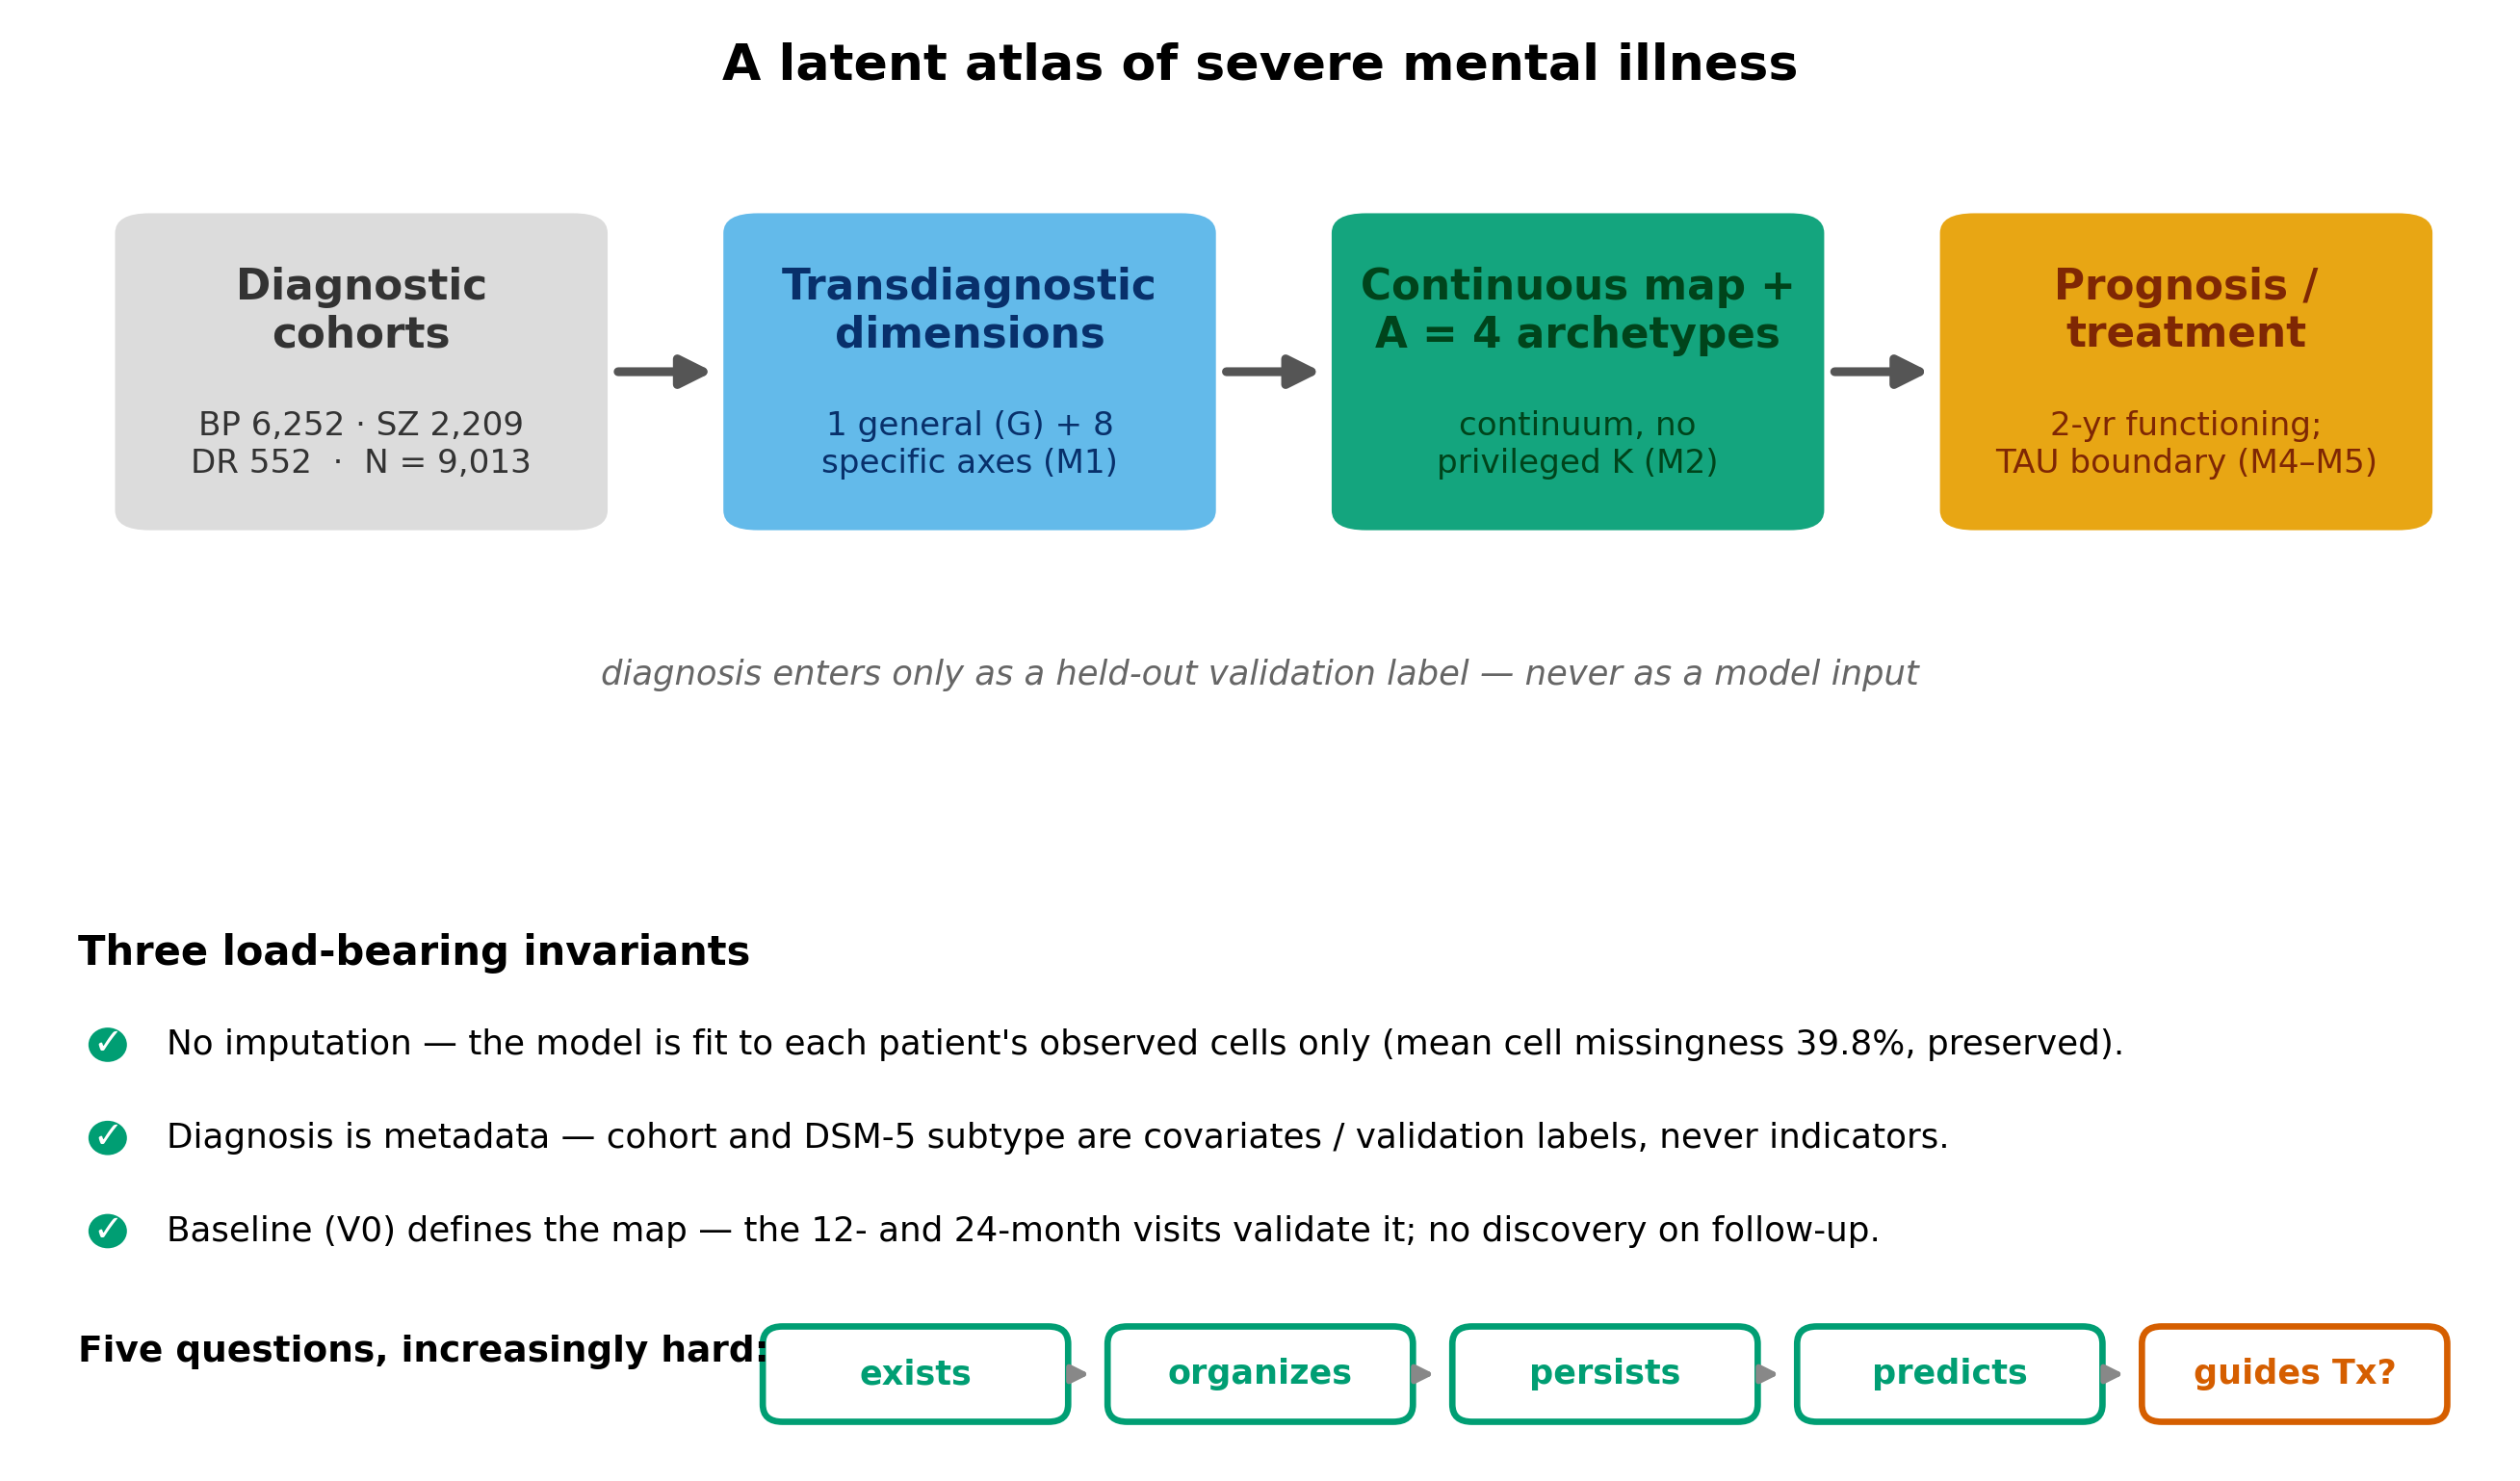
\includegraphics[width=0.95\linewidth]{fig1_overview.png}
  \caption{\textbf{Study design, invariants and the four questions.} The harmonized
  three-cohort FACE baseline (bipolar disorder, schizophrenia, depression;
  $N=9{,}013$) is reorganized around diagnosis-agnostic axes by one global,
  missingness-aware Bayesian bifactor / exploratory structural-equation model fit to
  each patient's observed cells only, under three core modelling principles (no
  imputation; diagnosis as metadata; baseline defines the map and follow-up validates
  it). The fitted map is then interrogated through four dependent, increasingly
  demanding questions---exists, organizes, persists, predicts---with
  positive and null results reported alike.}
  \label{fig:design}
\end{figure}

\begin{figure}[p]
  \centering
  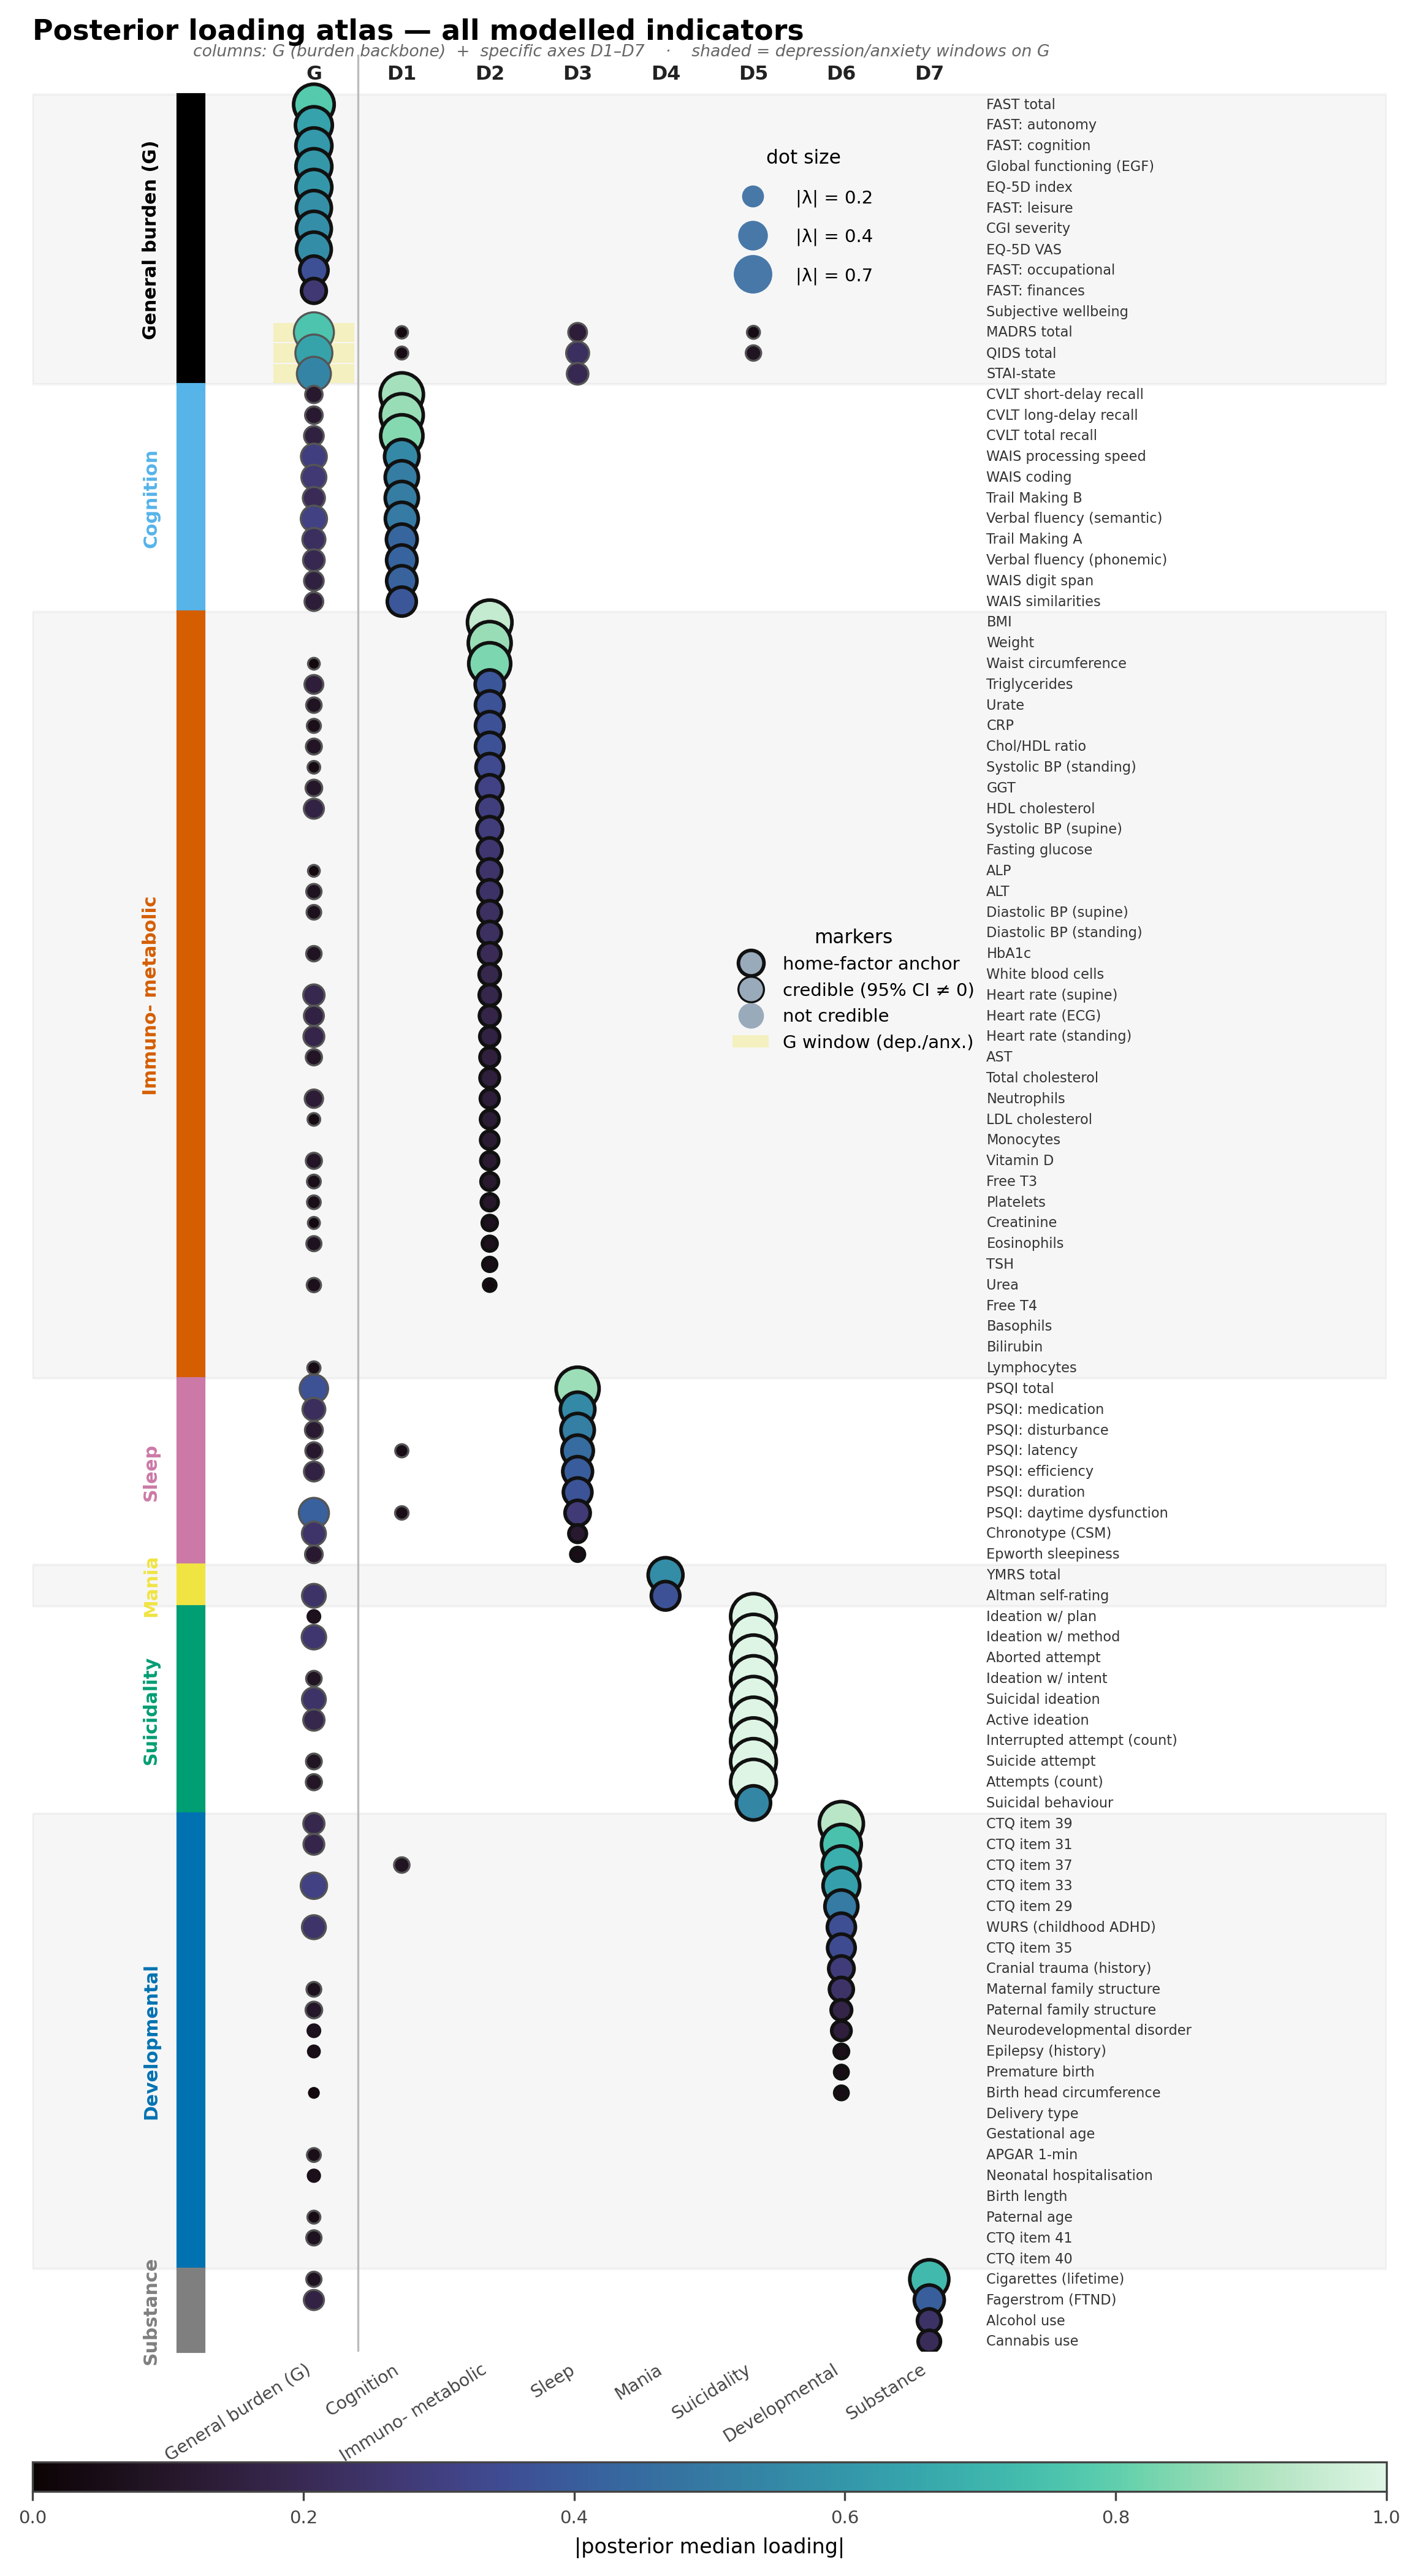
\includegraphics[height=0.86\textheight]{edfig_full_atlas.png}
  \caption{\textbf{The complete posterior loading atlas.} As Figure~\ref{fig:atlas}a but
  showing \emph{every} modelled indicator (all $109$ items: $88$ continuous and $21$ explicit) grouped
  by home factor, with no per-block cap. Dot size and colour encode the absolute posterior
  median loading; outlined dots have a $95\%$ credible interval excluding zero (heavier ring
  $=$ home-factor anchor). Three data-supported cross-loadings render as outlined dots in the
  cognition column---childhood adversity (CTQ-37, $-0.094$) and two poor-sleep items
  (PSQI latency $+0.057$, PSQI daytime dysfunction $-0.070$), each with a $95\%$ credible
  interval excluding zero. The diagonal block structure---each clinical block loading
  cleanly on its own specific axis, with a sparse general-burden ($\Gfac$) column---is the
  full anatomy of the measurement model summarised in the main-text Figure~\ref{fig:atlas}.}
  \label{fig:fullatlas}
\end{figure}

\begin{figure}[hbtp]
  \centering
  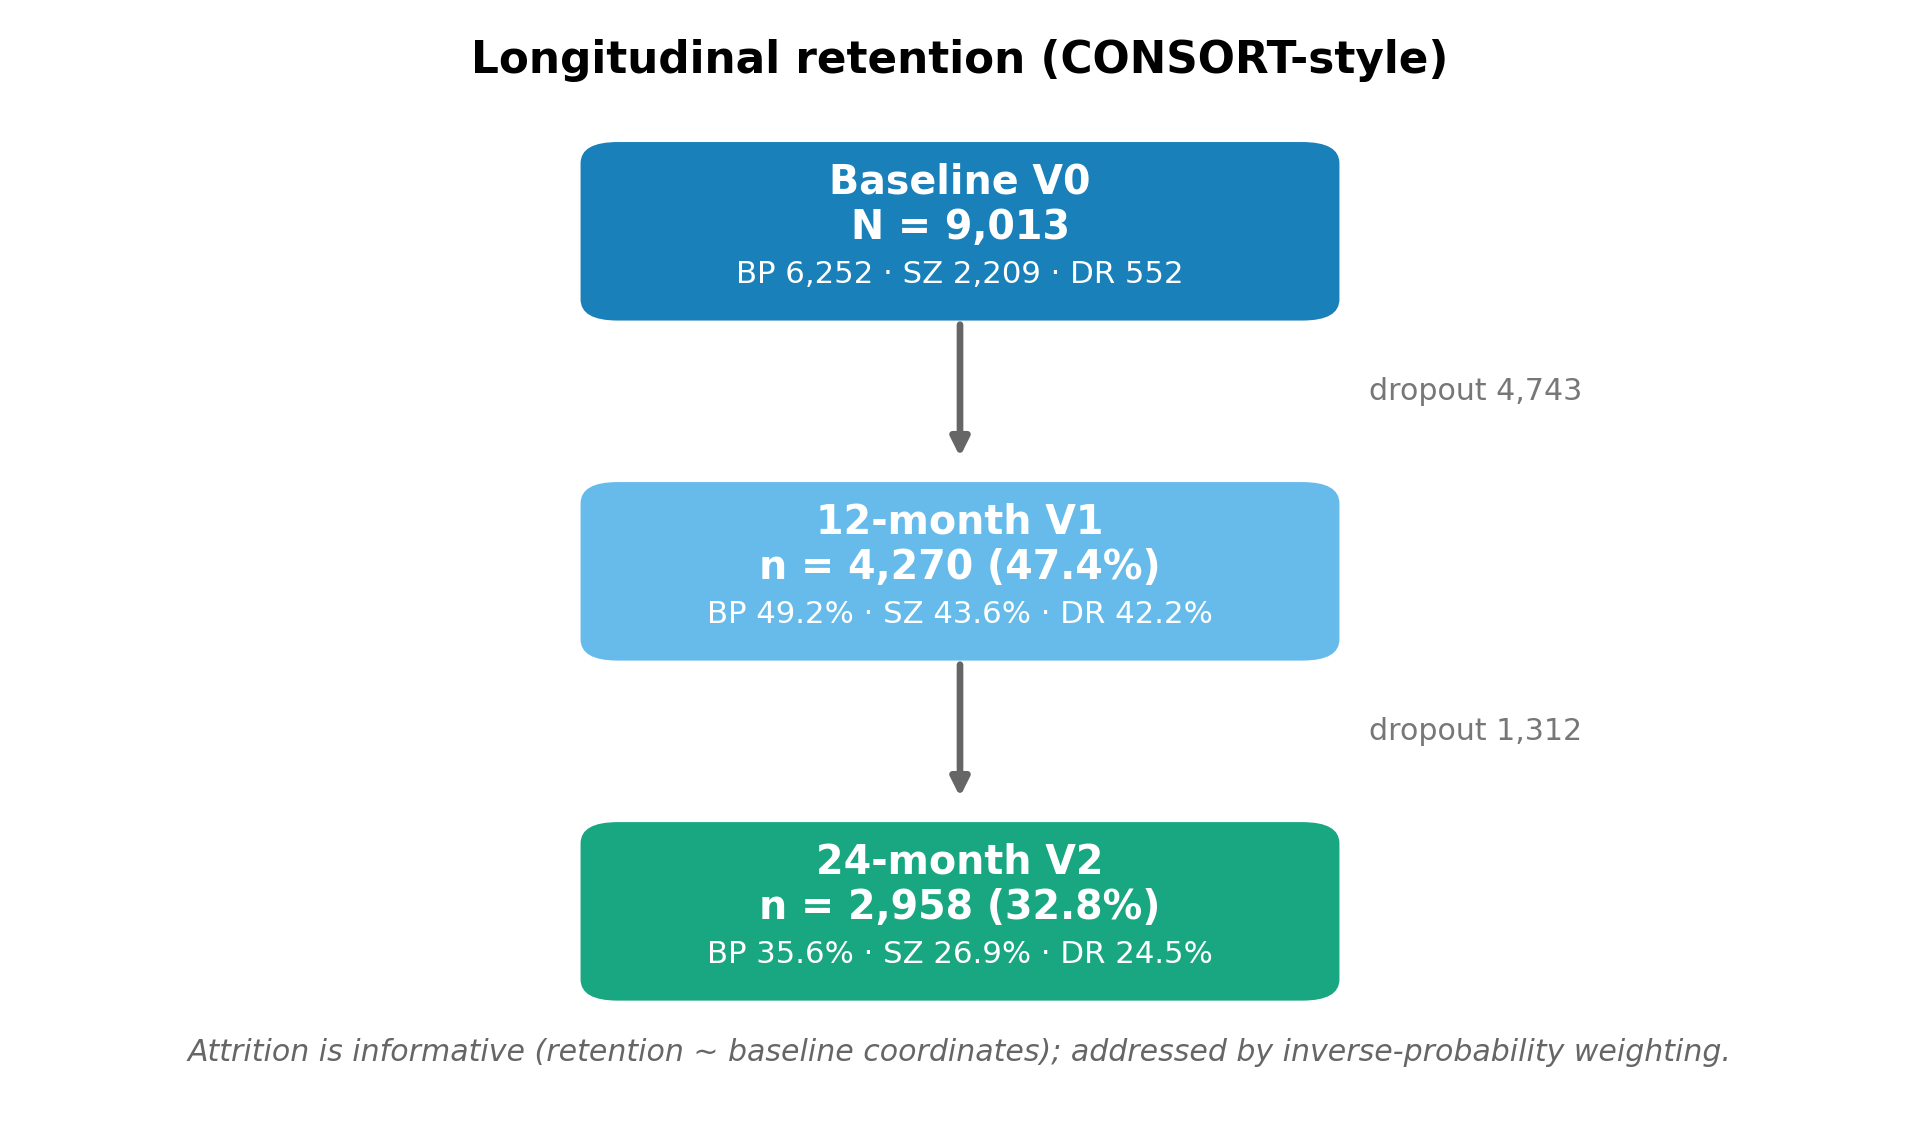
\includegraphics[width=0.72\linewidth]{edfig_consort.png}
  \caption{\textbf{Longitudinal retention.} Patients assessed at baseline and retained
  at the $12$- and $24$-month follow-up visits, overall and by cohort. Attrition is
  informative (retention depends on baseline coordinates) and is addressed throughout by
  inverse-probability weighting.}
  \label{fig:consort}
\end{figure}

\begin{figure}[hbtp]
  \centering
  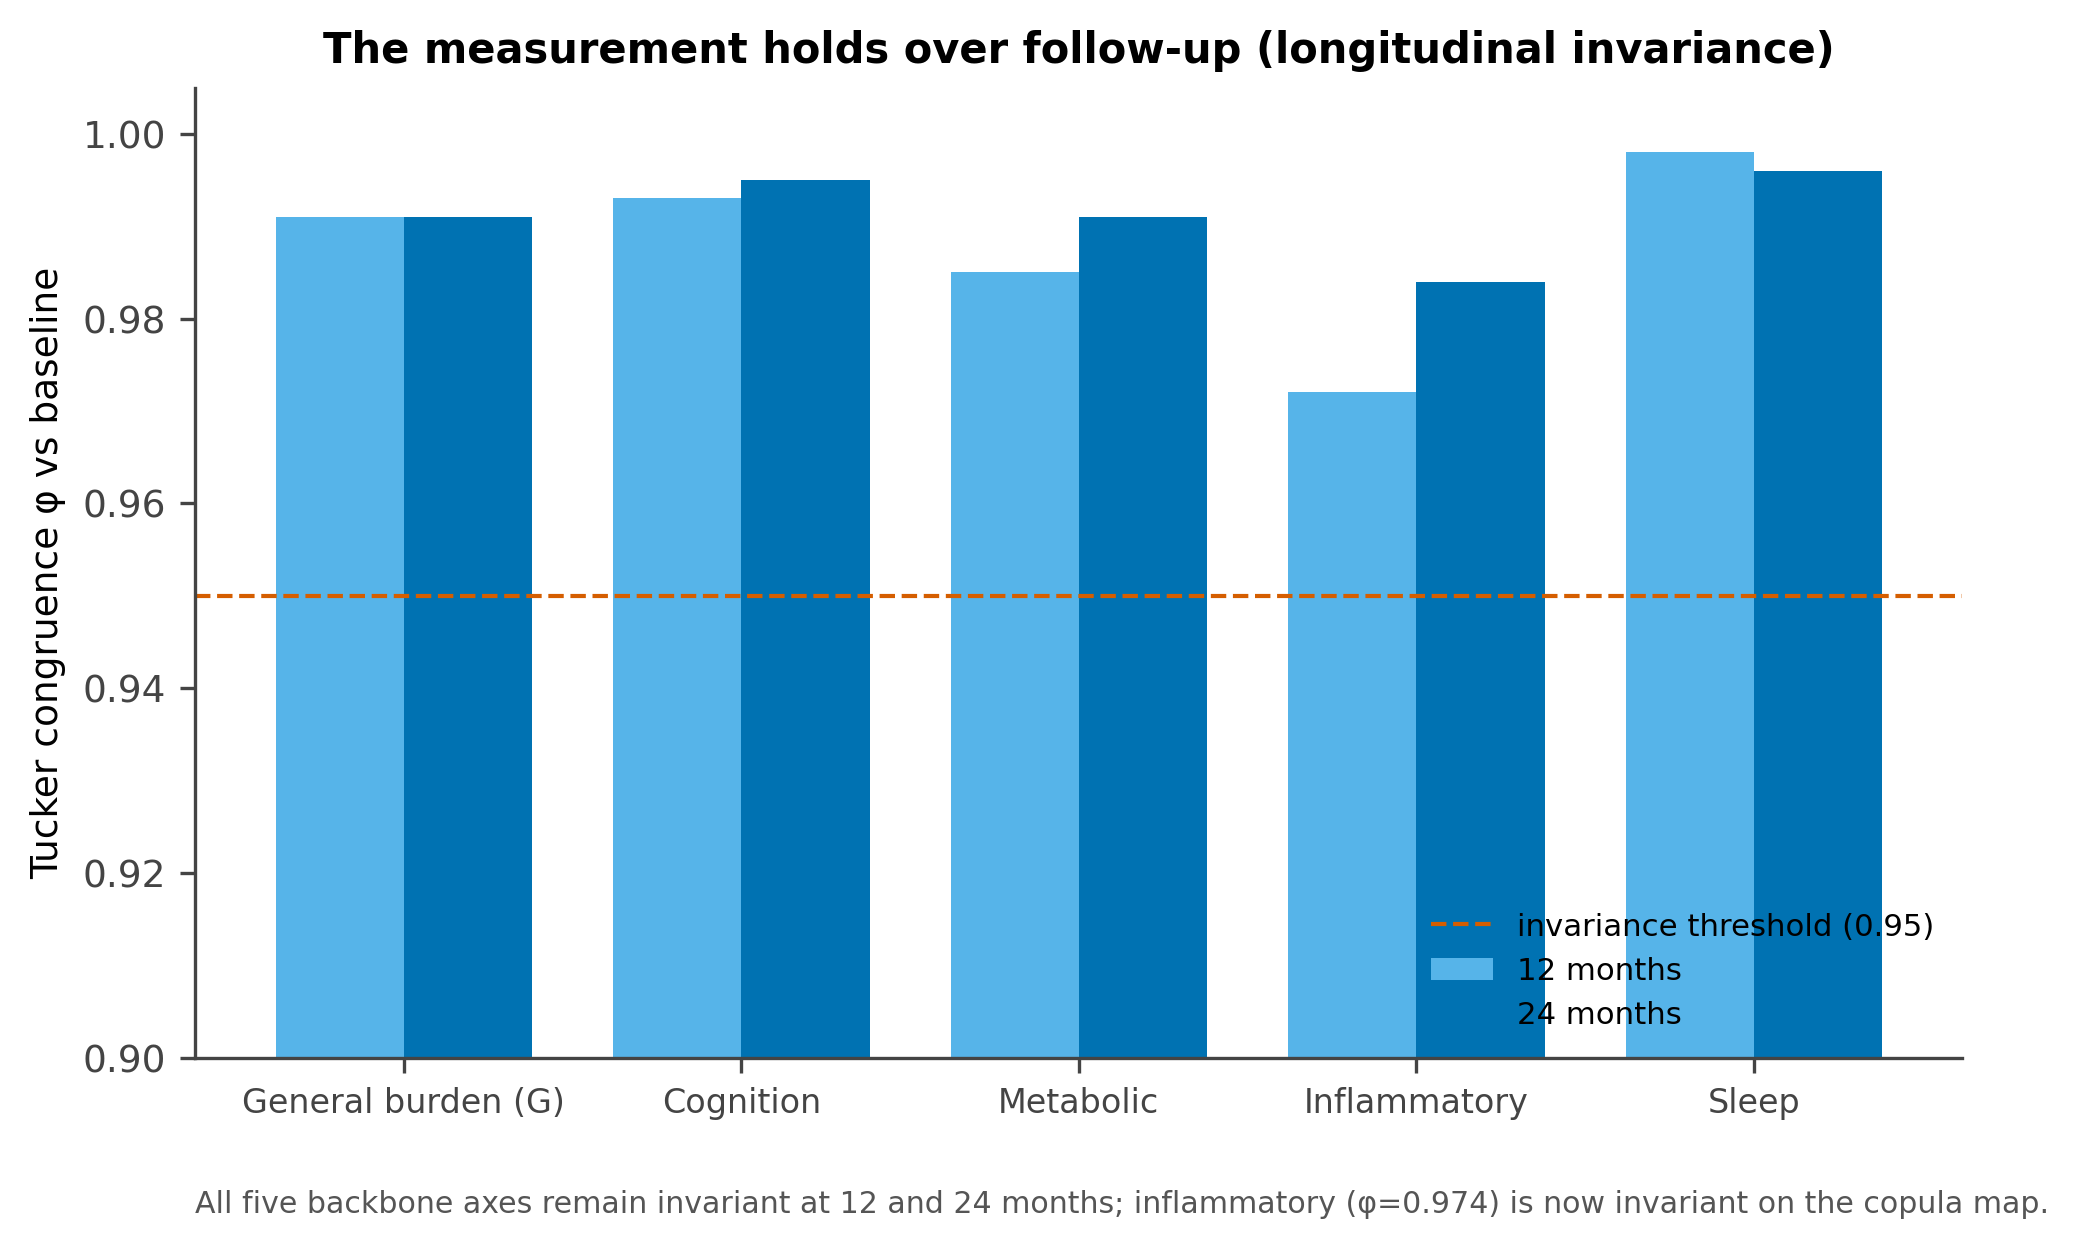
\includegraphics[width=0.72\linewidth]{edfig_invariance.png}
  \caption{\textbf{Longitudinal measurement invariance.} Tucker congruence of each
  backbone axis against baseline at $12$ and $24$ months. All four backbone axes
  (\Gfac, cognition, immunometabolic, sleep) remain invariant ($\varphi\ge0.95$); the
  merged immunometabolic biology axis is fully invariant ($\varphi=0.987$).}
  \label{fig:invariance}
\end{figure}

\begin{figure}[hbtp]
  \centering
  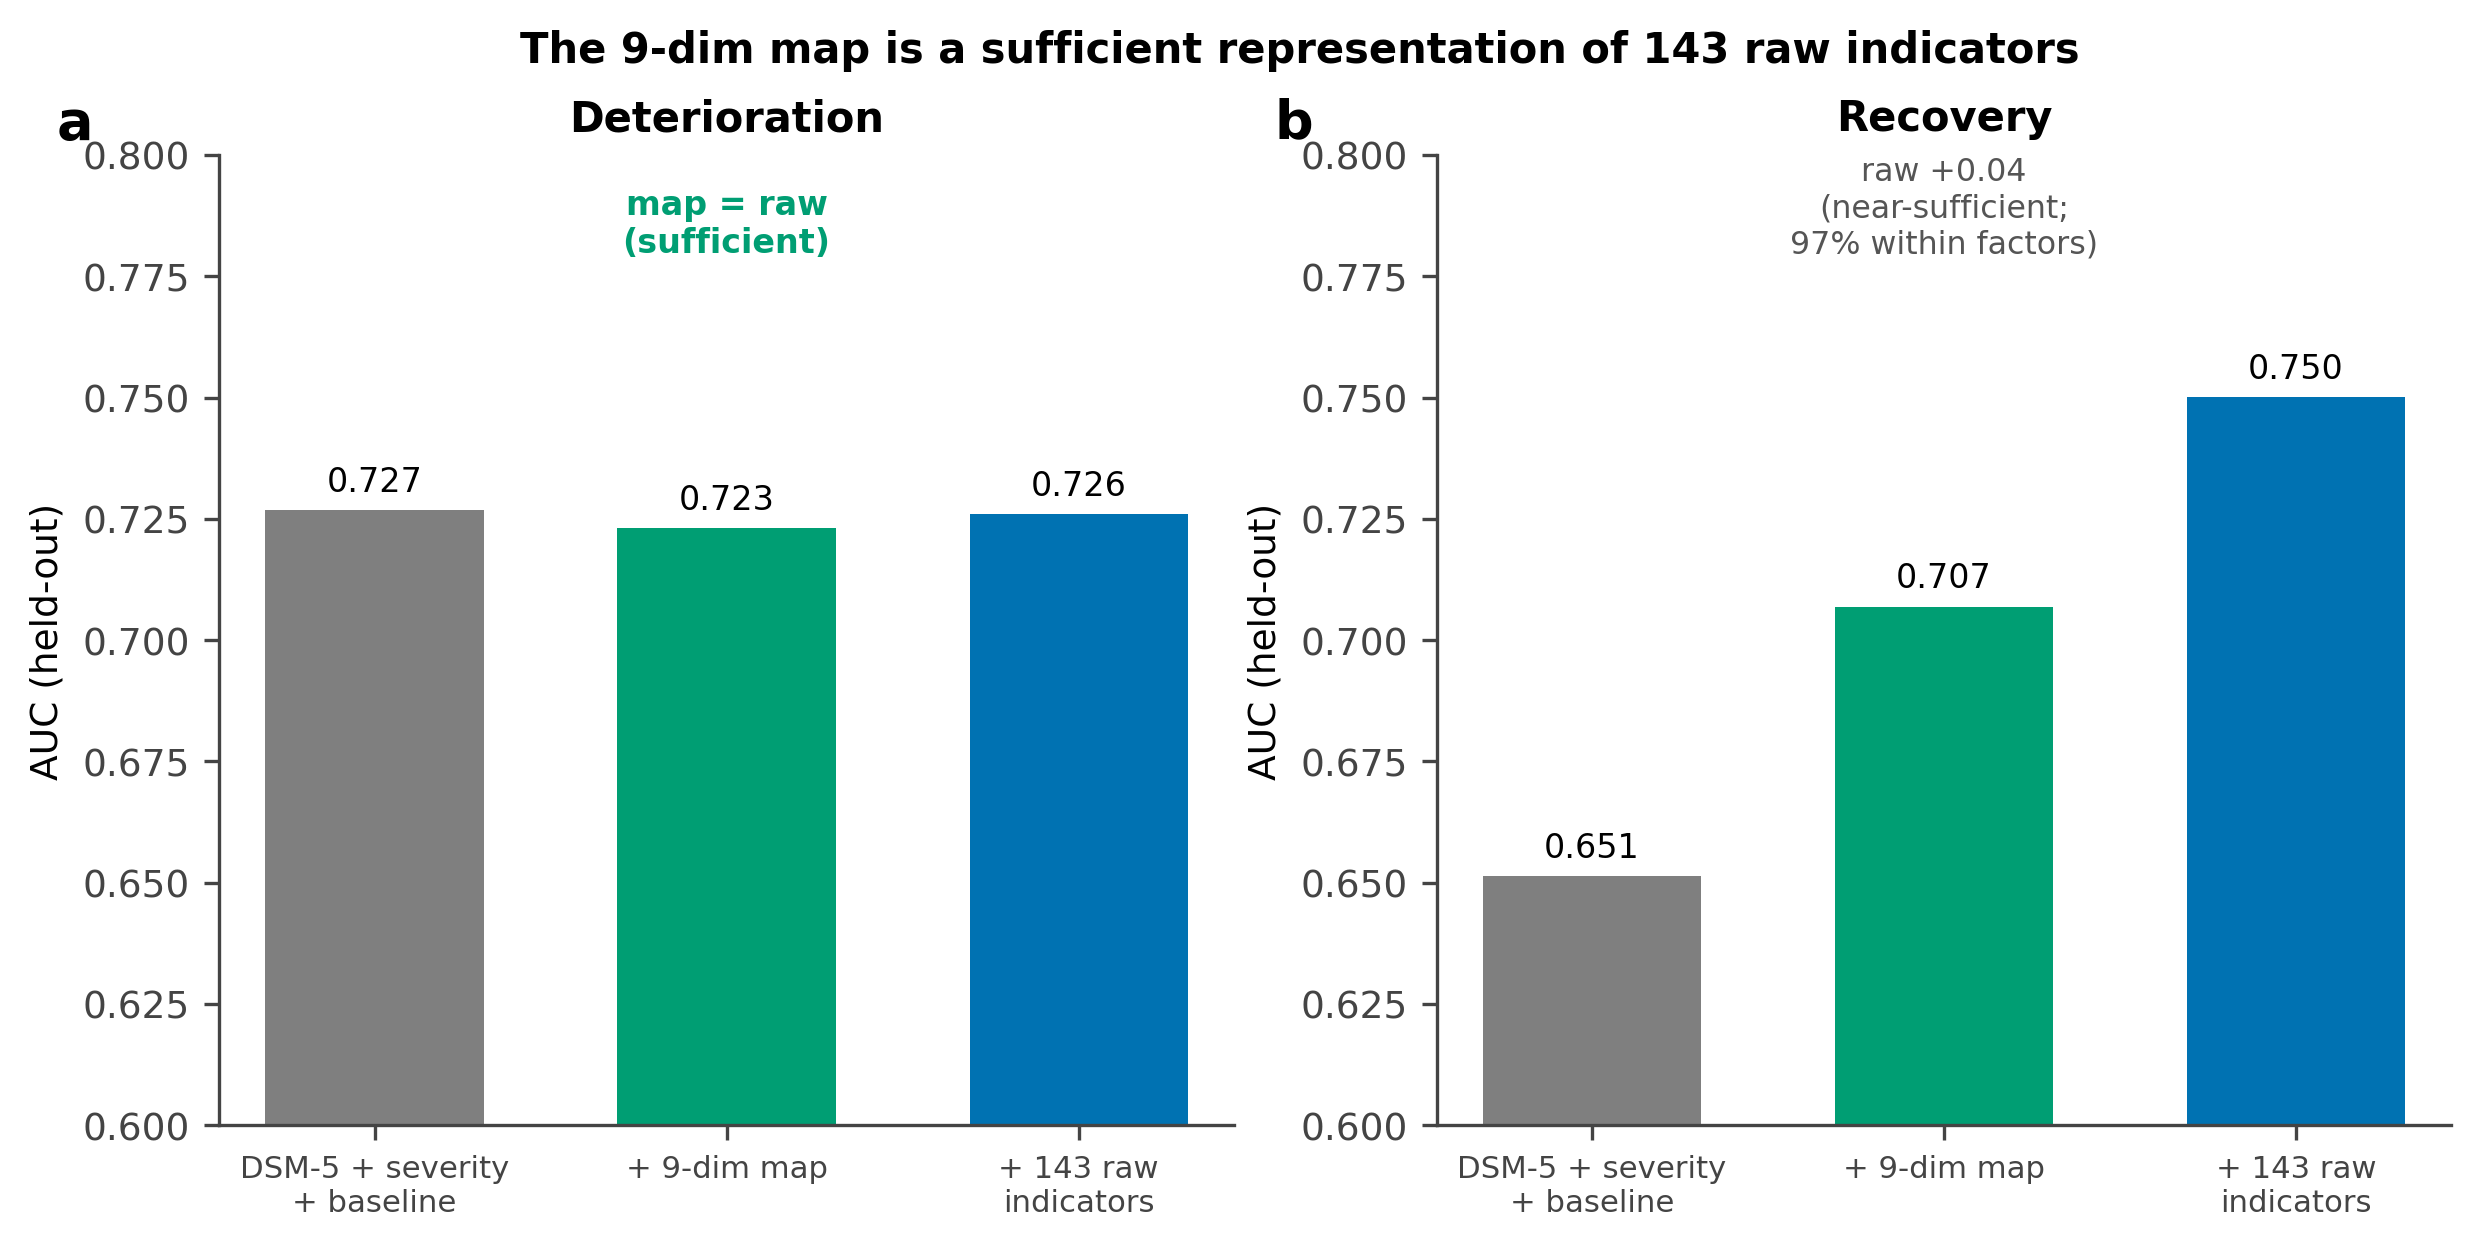
\includegraphics[width=0.85\linewidth]{edfig_repbench.png}
  \caption{\textbf{The eight-factor map is a sufficient representation of the $143$
  raw indicators.} Held-out AUC for a matched gradient-boosting classifier predicting
  two-year deterioration and recovery, using the reference (DSM-5 $+$ severity $+$
  baseline), the reference $+$ the eight-factor map, or the reference $+$ all $143$ raw
  indicators. The map equals the raw indicators for deterioration (sufficient) and
  trails by $\approx0.04$ AUC for recovery (near-sufficient); $\ge92\%$ of the raw recovery
  signal lies within the eight factors.}
  \label{fig:repbench}
\end{figure}

\begin{figure}[hbtp]
  \centering
  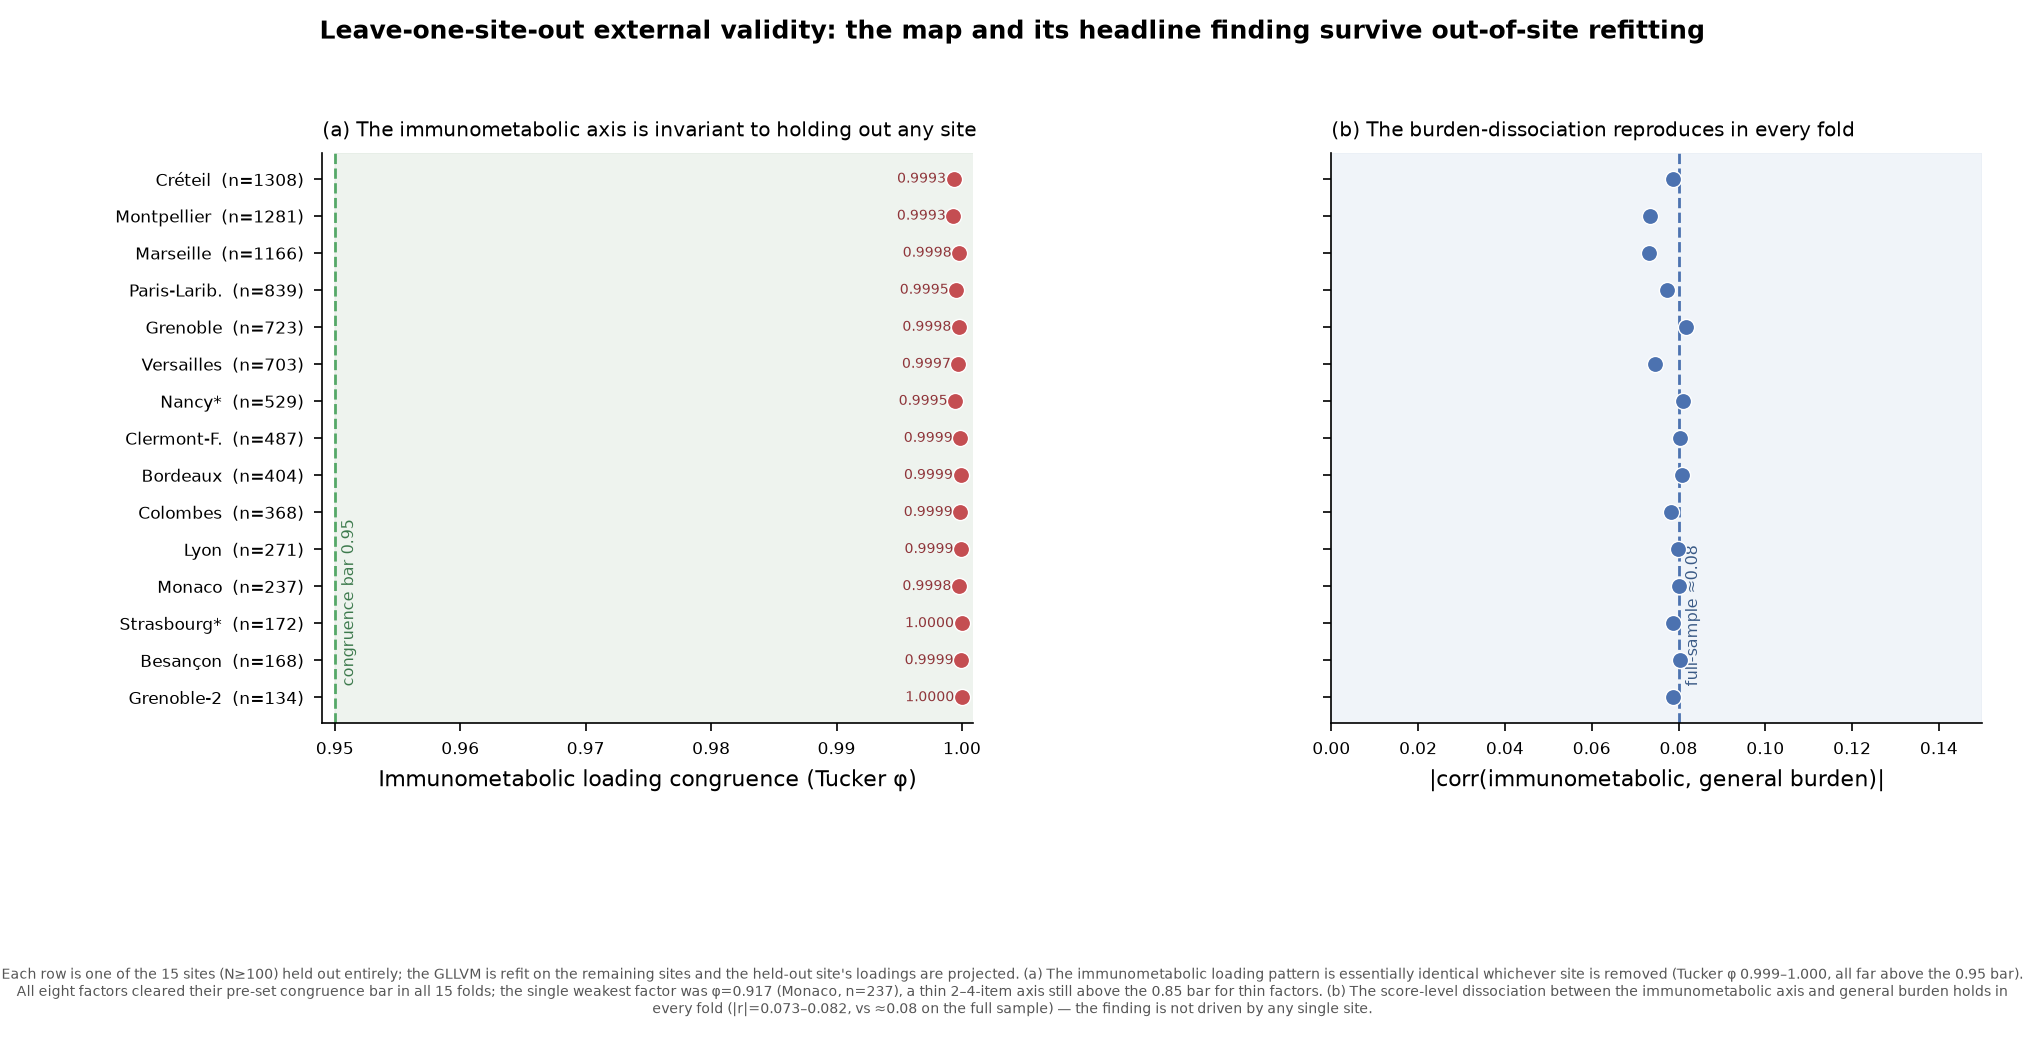
\includegraphics[width=0.95\linewidth]{edfig_loso.png}
  \caption{\textbf{Leave-one-site-out external validity: the map and its headline
  finding survive out-of-site refitting.} Each row is one of the 15 sites
  ($N\ge100$) held out entirely; the GLLVM is refit on the remaining sites and the
  held-out site's loadings are projected. \textbf{(a)}~The immunometabolic loading
  pattern is essentially identical whichever site is removed (Tucker
  $\varphi=0.999$--$1.000$, all far above the $0.95$ congruence bar). All eight
  factors cleared their pre-set congruence bar in all 15 folds; the single
  weakest factor was $\varphi=0.917$ (Monaco, $n=237$), a thin two-to-four-item
  axis still above the $0.85$ bar for thin factors. \textbf{(b)}~The score-level
  dissociation between the immunometabolic axis and general burden holds in
  every fold ($|r|=0.073$--$0.082$, versus $\approx0.08$ on the full sample)---the
  finding is not driven by any single site.}
  \label{fig:loso}
\end{figure}

\begin{figure}[hbtp]
  \centering
  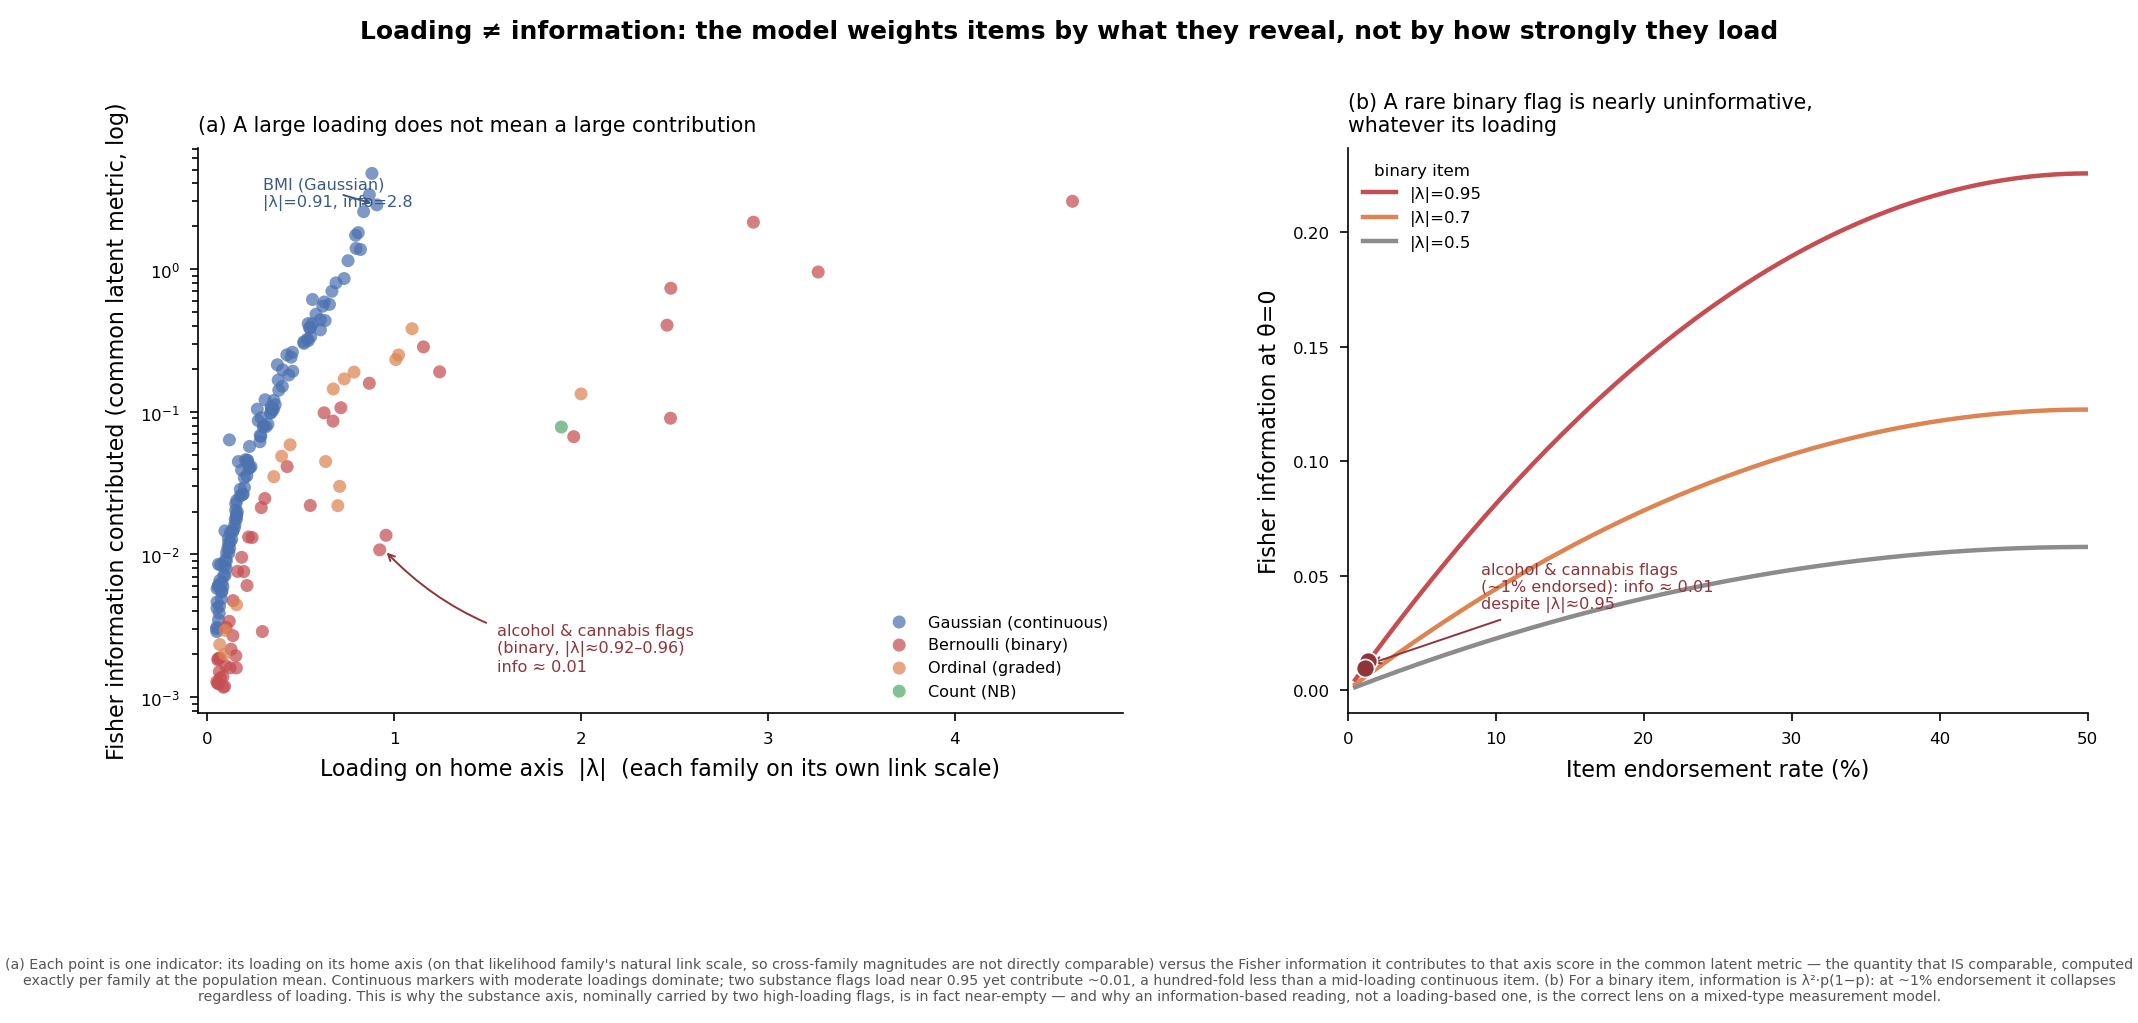
\includegraphics[width=0.95\linewidth]{fig_loading_vs_info.png}
  \caption{\textbf{Loading $\neq$ information: the model weighs items by what they
  reveal, not by how strongly they load.} \textbf{(a)}~Every indicator's loading on
  its home axis (on that likelihood family's own link scale, so cross-family
  magnitudes are not directly comparable) against the exact Fisher information it
  contributes to that axis score at the population mean---the quantity that
  \emph{is} comparable across families. Continuous markers with moderate loadings
  dominate; the two substance-use flags (alcohol, cannabis) load $\approx0.92$--$0.96$
  yet contribute only $\approx0.01$--$0.013$, roughly a hundred-fold less than a
  mid-loading continuous marker such as body-mass index (specific-factor loading
  $0.908$, information $2.8$; the table-reported general loading is $\approx0.95$).
  \textbf{(b)}~The mechanism: for a binary item, Fisher information is
  $\lambda^2 p(1-p)$, which collapses toward zero as endorsement approaches the
  extremes whatever the loading---so a rare binary flag is nearly uninformative
  regardless of how strongly it loads. This is why the substance-use axis, nominally
  carried by two high-loading flags, is in fact near-empty of information, and why an
  information-based reading of the map, not a loading-based one, is the correct lens
  on a mixed-type measurement model.}
  \label{fig:loadinginfo}
\end{figure}

\begin{figure}[hbtp]
  \centering
  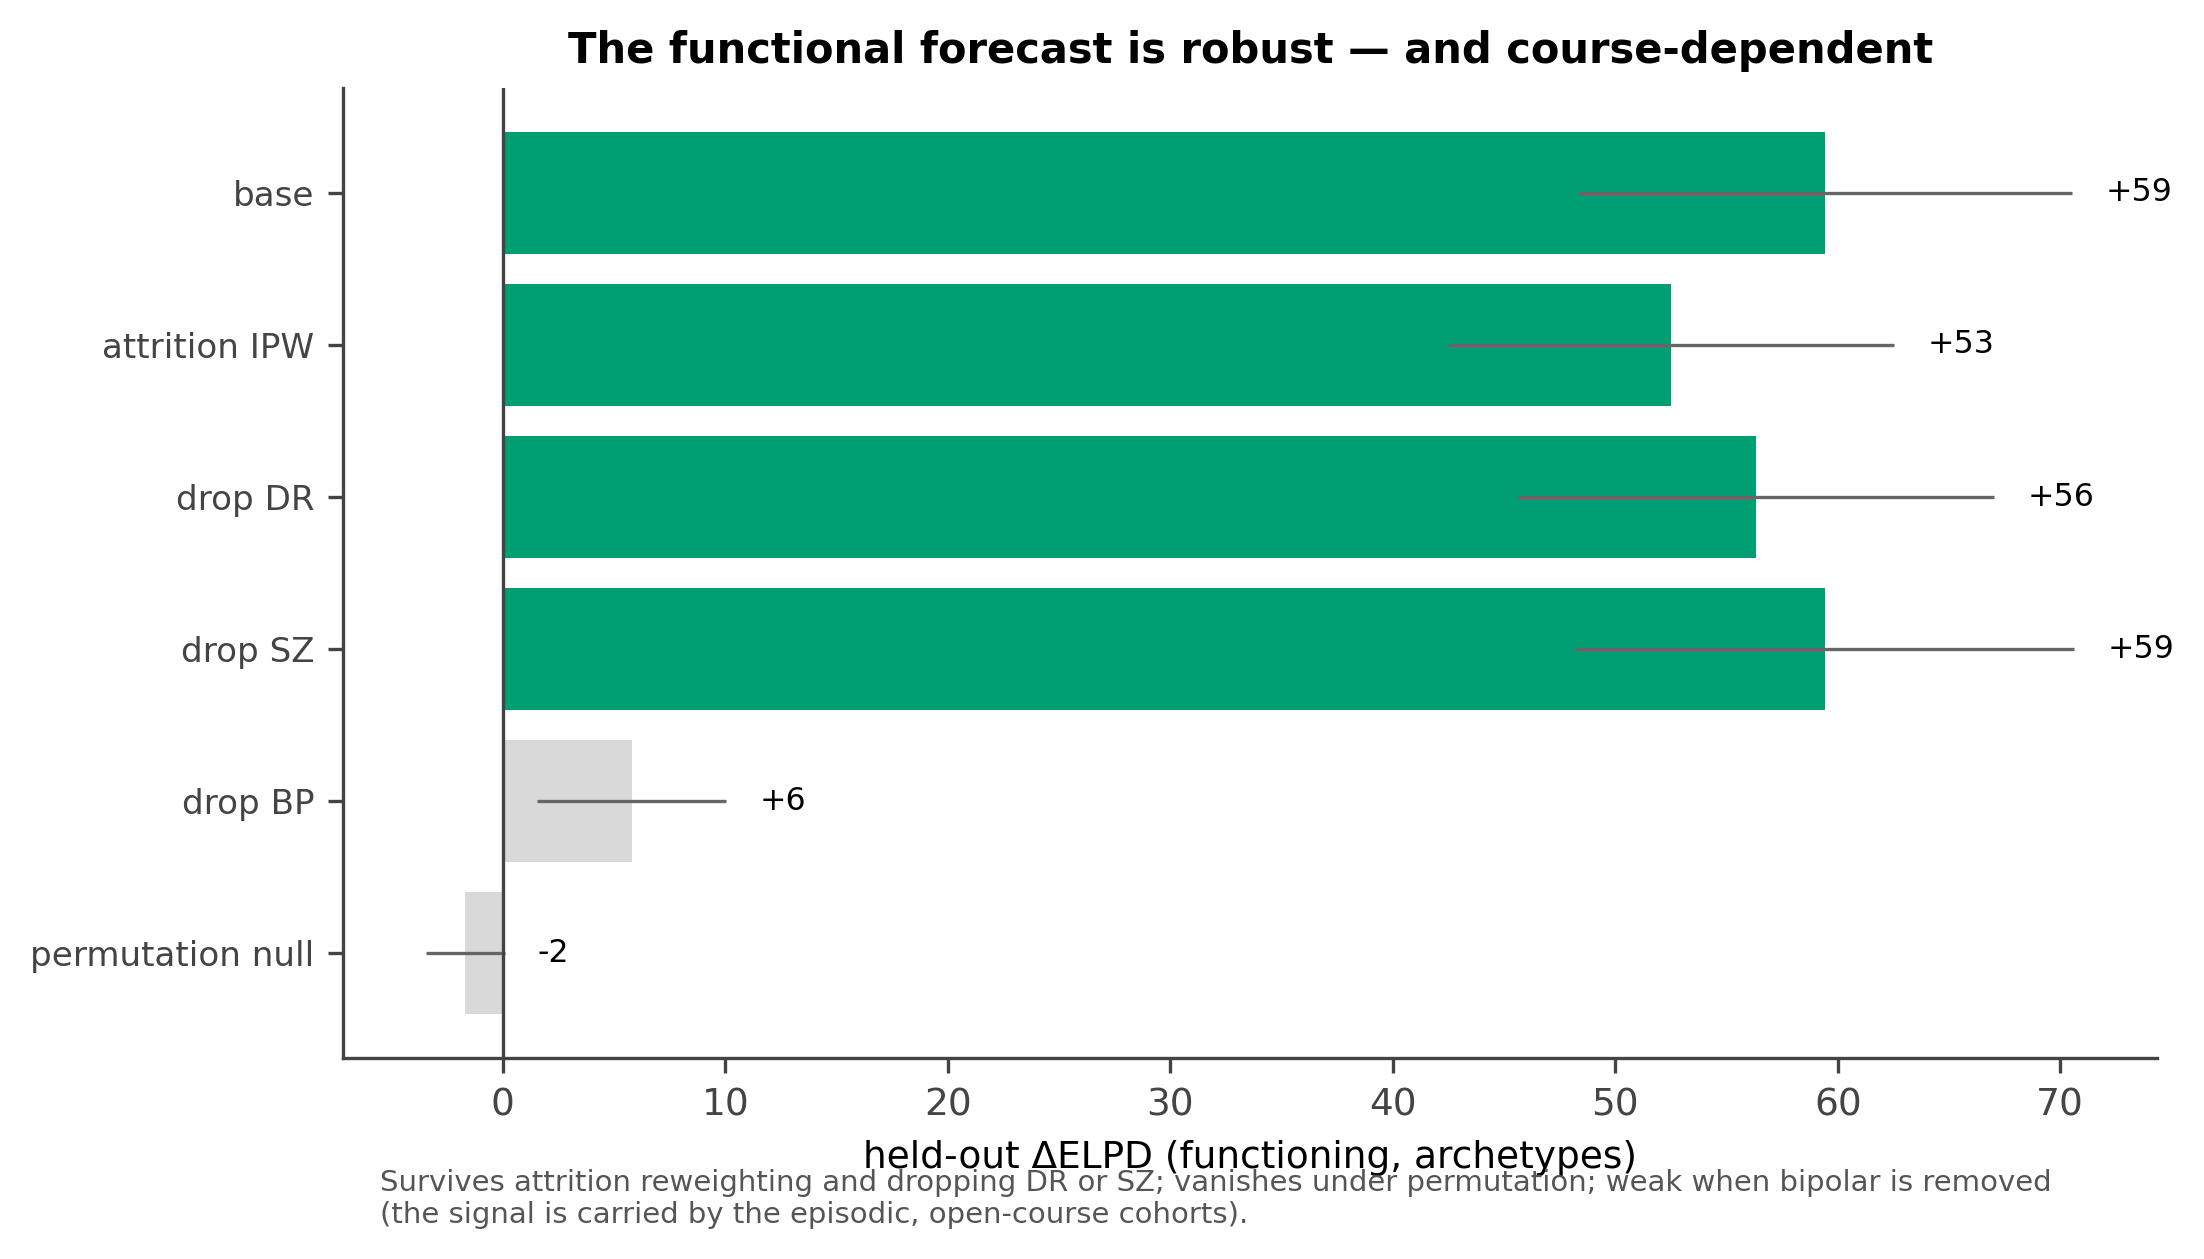
\includegraphics[width=0.72\linewidth]{edfig_robustness.png}
  \caption{\textbf{The functional forecast is robust and course-dependent.} Held-out
  incremental value of the archetype phenotype for two-year functioning under attrition
  reweighting, cohort hold-outs and a permutation null. The signal survives attrition and
  dropping either DR or SZ, vanishes under permutation, and weakens when bipolar disorder
  is removed---it is carried by the episodic, open-course cohorts.}
  \label{fig:robustness}
\end{figure}

\clearpage
\subsection{The claims ledger}

Table~\ref{tab:claims} states, side by side, what the study claims and what it
deliberately does not---the spine of the Limitations and of any response to reviewers.

\begin{table}[hbtp]
\centering
\caption{\textbf{What we claim, and what we do not.}}
\label{tab:claims}
\renewcommand{\arraystretch}{1.3}
\begin{tabular}{p{0.46\linewidth} p{0.46\linewidth}}
\toprule
\textbf{We claim} & \textbf{We do not claim} \\
\midrule
A validated eight-dimension transdiagnostic measurement map (internal validity). &
Natural biotypes or subtypes; that no biotype exists in any measurement space. \\
Immunometabolic load \emph{largely independent} of a general functional-burden
axis (quantified, with boundary conditions). &
Strict statistical orthogonality, or independence from \emph{being ill}
(case--control elevations). \\
A graded continuum, resolved by five stable archetypes, that is descriptively
tighter than DSM-5. &
That the regions are clinically superior to DSM-5 beyond the modest prognostic
increment shown. \\
Temporal coherence: durable biology, moving symptoms. &
That developmental risk is genuinely ``state'' (it partly reflects recall noise). \\
A modest, \emph{group-level} incremental prognosis for \emph{functioning}, carried by
the biological phenotype, course-dependent. &
A large individual-risk gain; prediction of \emph{recorded} relapse/hospitalization
events; a deployable individual rule. \\
Convergent validity with the immuno-metabolic literature. &
External or out-of-sample validation (none yet). \\
\bottomrule
\end{tabular}
\end{table}


%================================ REFERENCES ==================================
\bibliographystyle{unsrtnat}
\bibliography{references}

\end{document}
